\documentclass[11pt]{article}

% Shared packages, settings, and macros (see preamble.tex)
% ============================================================
% Shared preamble for the B. glandula genome manuscript.
%
% Included (via % ============================================================
% Shared preamble for the B. glandula genome manuscript.
%
% Included (via % ============================================================
% Shared preamble for the B. glandula genome manuscript.
%
% Included (via \input{preamble}) by main.tex, submission_main.tex,
% and submission_sups.tex, immediately after \documentclass. This
% is done here to avoid sync issues between the main and submission
% documents. Any file-specific settings are done locally
% ============================================================

\usepackage{graphicx} % Required for inserting images
\usepackage[utf8]{inputenc}
\usepackage[letterpaper,margin=1.0in]{geometry}
%% Some formatting stuff
\usepackage{authblk}
\usepackage{fancyhdr}
\usepackage{lineno}
\usepackage{siunitx}
\usepackage{hyperref}
\usepackage{booktabs}
\usepackage{textgreek}
\setlength{\headheight}{13.59999pt}
\pagestyle{fancy}
\fancyhead[R]{\textbf{Rivera-Col\'{o}n \textit{et al.} 2026 - \textit{B. glandula} genome}}
% for figures
\usepackage{graphicx}
\usepackage{wrapfig}
\usepackage{breakcites}
\usepackage{nameref}
\usepackage{amsmath}
\usepackage{lipsum}
\usepackage{rotating}
\usepackage{xspace}
\usepackage{fixltx2e}
% for highlighting text
\usepackage{xcolor}
\usepackage{soul}
\usepackage[dvipsnames]{xcolor}
\usepackage{caption}
\usepackage[T1]{fontenc}
\usepackage{lmodern}

% For supplemental figure and table numbering
\newcounter{supfigure}
\newcounter{suptable}

% Commands for supplemental tables and figures
\newcommand{\suptablecaption}[1]{%
    \refstepcounter{suptable}% Step forward our supplemental counter
    \renewcommand{\thetable}{S\arabic{suptable}}% Temporarily change table numbering
    \caption{#1}%
    \renewcommand{\thetable}{\arabic{table}}% Restore normal table numbering
}

\newcommand{\supfigurecaption}[1]{%
    \refstepcounter{supfigure}% Step forward our supplemental counter
    \renewcommand{\thefigure}{S\arabic{supfigure}}% Temporarily change figure numbering
    \caption{#1}%
    \renewcommand{\thefigure}{\arabic{figure}}% Restore normal figure numbering
}

% Colors for hyperlinks and other things
\hypersetup{
    colorlinks=true,
    citecolor=MidnightBlue,
    urlcolor=RoyalBlue,
    linkcolor=Blue
}
\setstcolor{Red}
\urlstyle{same}

% For the citations
\usepackage[backend=biber, style=apa, natbib=true,
    doi=true, url=true, eprint=true, isbn=false]{biblatex}
\addbibresource{references/references.bib}

% Some aliases for text
\newcommand{\dnds}{d\textsubscript{N}/d\textsubscript{S}\xspace}
\newcommand{\balgla}{\textit{Balanus glandula}\xspace}
\newcommand{\bgla}{\textit{B. glandula}\xspace}
\newcommand{\Ne}{N\textsubscript{e}\xspace}
\newcommand{\Ks}{K\textsubscript{S}\xspace}
\newcommand{\wrightenc}{$\text{ENC}_{exp} = 2 + s + 29/[s^{2} + (1-s)^{2}]$\xspace}
\newcommand{\comment}[1]{{\color{PineGreen} #1}}
\newcommand{\commentauth}[2]{{\color{RedViolet} \underline{#1:} #2}}
) by main.tex, submission_main.tex,
% and submission_sups.tex, immediately after \documentclass. This
% is done here to avoid sync issues between the main and submission
% documents. Any file-specific settings are done locally
% ============================================================

\usepackage{graphicx} % Required for inserting images
\usepackage[utf8]{inputenc}
\usepackage[letterpaper,margin=1.0in]{geometry}
%% Some formatting stuff
\usepackage{authblk}
\usepackage{fancyhdr}
\usepackage{lineno}
\usepackage{siunitx}
\usepackage{hyperref}
\usepackage{booktabs}
\usepackage{textgreek}
\setlength{\headheight}{13.59999pt}
\pagestyle{fancy}
\fancyhead[R]{\textbf{Rivera-Col\'{o}n \textit{et al.} 2026 - \textit{B. glandula} genome}}
% for figures
\usepackage{graphicx}
\usepackage{wrapfig}
\usepackage{breakcites}
\usepackage{nameref}
\usepackage{amsmath}
\usepackage{lipsum}
\usepackage{rotating}
\usepackage{xspace}
\usepackage{fixltx2e}
% for highlighting text
\usepackage{xcolor}
\usepackage{soul}
\usepackage[dvipsnames]{xcolor}
\usepackage{caption}
\usepackage[T1]{fontenc}
\usepackage{lmodern}

% For supplemental figure and table numbering
\newcounter{supfigure}
\newcounter{suptable}

% Commands for supplemental tables and figures
\newcommand{\suptablecaption}[1]{%
    \refstepcounter{suptable}% Step forward our supplemental counter
    \renewcommand{\thetable}{S\arabic{suptable}}% Temporarily change table numbering
    \caption{#1}%
    \renewcommand{\thetable}{\arabic{table}}% Restore normal table numbering
}

\newcommand{\supfigurecaption}[1]{%
    \refstepcounter{supfigure}% Step forward our supplemental counter
    \renewcommand{\thefigure}{S\arabic{supfigure}}% Temporarily change figure numbering
    \caption{#1}%
    \renewcommand{\thefigure}{\arabic{figure}}% Restore normal figure numbering
}

% Colors for hyperlinks and other things
\hypersetup{
    colorlinks=true,
    citecolor=MidnightBlue,
    urlcolor=RoyalBlue,
    linkcolor=Blue
}
\setstcolor{Red}
\urlstyle{same}

% For the citations
\usepackage[backend=biber, style=apa, natbib=true,
    doi=true, url=true, eprint=true, isbn=false]{biblatex}
\addbibresource{references/references.bib}

% Some aliases for text
\newcommand{\dnds}{d\textsubscript{N}/d\textsubscript{S}\xspace}
\newcommand{\balgla}{\textit{Balanus glandula}\xspace}
\newcommand{\bgla}{\textit{B. glandula}\xspace}
\newcommand{\Ne}{N\textsubscript{e}\xspace}
\newcommand{\Ks}{K\textsubscript{S}\xspace}
\newcommand{\wrightenc}{$\text{ENC}_{exp} = 2 + s + 29/[s^{2} + (1-s)^{2}]$\xspace}
\newcommand{\comment}[1]{{\color{PineGreen} #1}}
\newcommand{\commentauth}[2]{{\color{RedViolet} \underline{#1:} #2}}
) by main.tex, submission_main.tex,
% and submission_sups.tex, immediately after \documentclass. This
% is done here to avoid sync issues between the main and submission
% documents. Any file-specific settings are done locally
% ============================================================

\usepackage{graphicx} % Required for inserting images
\usepackage[utf8]{inputenc}
\usepackage[letterpaper,margin=1.0in]{geometry}
%% Some formatting stuff
\usepackage{authblk}
\usepackage{fancyhdr}
\usepackage{lineno}
\usepackage{siunitx}
\usepackage{hyperref}
\usepackage{booktabs}
\usepackage{textgreek}
\setlength{\headheight}{13.59999pt}
\pagestyle{fancy}
\fancyhead[R]{\textbf{Rivera-Col\'{o}n \textit{et al.} 2026 - \textit{B. glandula} genome}}
% for figures
\usepackage{graphicx}
\usepackage{wrapfig}
\usepackage{breakcites}
\usepackage{nameref}
\usepackage{amsmath}
\usepackage{lipsum}
\usepackage{rotating}
\usepackage{xspace}
\usepackage{fixltx2e}
% for highlighting text
\usepackage{xcolor}
\usepackage{soul}
\usepackage[dvipsnames]{xcolor}
\usepackage{caption}
\usepackage[T1]{fontenc}
\usepackage{lmodern}

% For supplemental figure and table numbering
\newcounter{supfigure}
\newcounter{suptable}

% Commands for supplemental tables and figures
\newcommand{\suptablecaption}[1]{%
    \refstepcounter{suptable}% Step forward our supplemental counter
    \renewcommand{\thetable}{S\arabic{suptable}}% Temporarily change table numbering
    \caption{#1}%
    \renewcommand{\thetable}{\arabic{table}}% Restore normal table numbering
}

\newcommand{\supfigurecaption}[1]{%
    \refstepcounter{supfigure}% Step forward our supplemental counter
    \renewcommand{\thefigure}{S\arabic{supfigure}}% Temporarily change figure numbering
    \caption{#1}%
    \renewcommand{\thefigure}{\arabic{figure}}% Restore normal figure numbering
}

% Colors for hyperlinks and other things
\hypersetup{
    colorlinks=true,
    citecolor=MidnightBlue,
    urlcolor=RoyalBlue,
    linkcolor=Blue
}
\setstcolor{Red}
\urlstyle{same}

% For the citations
\usepackage[backend=biber, style=apa, natbib=true,
    doi=true, url=true, eprint=true, isbn=false]{biblatex}
\addbibresource{references/references.bib}

% Some aliases for text
\newcommand{\dnds}{d\textsubscript{N}/d\textsubscript{S}\xspace}
\newcommand{\balgla}{\textit{Balanus glandula}\xspace}
\newcommand{\bgla}{\textit{B. glandula}\xspace}
\newcommand{\Ne}{N\textsubscript{e}\xspace}
\newcommand{\Ks}{K\textsubscript{S}\xspace}
\newcommand{\wrightenc}{$\text{ENC}_{exp} = 2 + s + 29/[s^{2} + (1-s)^{2}]$\xspace}
\newcommand{\comment}[1]{{\color{PineGreen} #1}}
\newcommand{\commentauth}[2]{{\color{RedViolet} \underline{#1:} #2}}


% Shared title, authors, and affiliations (see title_authors.tex)
% Shared title, author list, and affiliations, included by main.tex,
% submission_main.tex, and submission_sups.tex so the three documents cannot
% drift apart. Edit here only.
%
% Input this after % ============================================================
% Shared preamble for the B. glandula genome manuscript.
%
% Included (via % ============================================================
% Shared preamble for the B. glandula genome manuscript.
%
% Included (via \input{preamble}) by main.tex, submission_main.tex,
% and submission_sups.tex, immediately after \documentclass. This
% is done here to avoid sync issues between the main and submission
% documents. Any file-specific settings are done locally
% ============================================================

\usepackage{graphicx} % Required for inserting images
\usepackage[utf8]{inputenc}
\usepackage[letterpaper,margin=1.0in]{geometry}
%% Some formatting stuff
\usepackage{authblk}
\usepackage{fancyhdr}
\usepackage{lineno}
\usepackage{siunitx}
\usepackage{hyperref}
\usepackage{booktabs}
\usepackage{textgreek}
\setlength{\headheight}{13.59999pt}
\pagestyle{fancy}
\fancyhead[R]{\textbf{Rivera-Col\'{o}n \textit{et al.} 2026 - \textit{B. glandula} genome}}
% for figures
\usepackage{graphicx}
\usepackage{wrapfig}
\usepackage{breakcites}
\usepackage{nameref}
\usepackage{amsmath}
\usepackage{lipsum}
\usepackage{rotating}
\usepackage{xspace}
\usepackage{fixltx2e}
% for highlighting text
\usepackage{xcolor}
\usepackage{soul}
\usepackage[dvipsnames]{xcolor}
\usepackage{caption}
\usepackage[T1]{fontenc}
\usepackage{lmodern}

% For supplemental figure and table numbering
\newcounter{supfigure}
\newcounter{suptable}

% Commands for supplemental tables and figures
\newcommand{\suptablecaption}[1]{%
    \refstepcounter{suptable}% Step forward our supplemental counter
    \renewcommand{\thetable}{S\arabic{suptable}}% Temporarily change table numbering
    \caption{#1}%
    \renewcommand{\thetable}{\arabic{table}}% Restore normal table numbering
}

\newcommand{\supfigurecaption}[1]{%
    \refstepcounter{supfigure}% Step forward our supplemental counter
    \renewcommand{\thefigure}{S\arabic{supfigure}}% Temporarily change figure numbering
    \caption{#1}%
    \renewcommand{\thefigure}{\arabic{figure}}% Restore normal figure numbering
}

% Colors for hyperlinks and other things
\hypersetup{
    colorlinks=true,
    citecolor=MidnightBlue,
    urlcolor=RoyalBlue,
    linkcolor=Blue
}
\setstcolor{Red}
\urlstyle{same}

% For the citations
\usepackage[backend=biber, style=apa, natbib=true,
    doi=true, url=true, eprint=true, isbn=false]{biblatex}
\addbibresource{references/references.bib}

% Some aliases for text
\newcommand{\dnds}{d\textsubscript{N}/d\textsubscript{S}\xspace}
\newcommand{\balgla}{\textit{Balanus glandula}\xspace}
\newcommand{\bgla}{\textit{B. glandula}\xspace}
\newcommand{\Ne}{N\textsubscript{e}\xspace}
\newcommand{\Ks}{K\textsubscript{S}\xspace}
\newcommand{\wrightenc}{$\text{ENC}_{exp} = 2 + s + 29/[s^{2} + (1-s)^{2}]$\xspace}
\newcommand{\comment}[1]{{\color{PineGreen} #1}}
\newcommand{\commentauth}[2]{{\color{RedViolet} \underline{#1:} #2}}
) by main.tex, submission_main.tex,
% and submission_sups.tex, immediately after \documentclass. This
% is done here to avoid sync issues between the main and submission
% documents. Any file-specific settings are done locally
% ============================================================

\usepackage{graphicx} % Required for inserting images
\usepackage[utf8]{inputenc}
\usepackage[letterpaper,margin=1.0in]{geometry}
%% Some formatting stuff
\usepackage{authblk}
\usepackage{fancyhdr}
\usepackage{lineno}
\usepackage{siunitx}
\usepackage{hyperref}
\usepackage{booktabs}
\usepackage{textgreek}
\setlength{\headheight}{13.59999pt}
\pagestyle{fancy}
\fancyhead[R]{\textbf{Rivera-Col\'{o}n \textit{et al.} 2026 - \textit{B. glandula} genome}}
% for figures
\usepackage{graphicx}
\usepackage{wrapfig}
\usepackage{breakcites}
\usepackage{nameref}
\usepackage{amsmath}
\usepackage{lipsum}
\usepackage{rotating}
\usepackage{xspace}
\usepackage{fixltx2e}
% for highlighting text
\usepackage{xcolor}
\usepackage{soul}
\usepackage[dvipsnames]{xcolor}
\usepackage{caption}
\usepackage[T1]{fontenc}
\usepackage{lmodern}

% For supplemental figure and table numbering
\newcounter{supfigure}
\newcounter{suptable}

% Commands for supplemental tables and figures
\newcommand{\suptablecaption}[1]{%
    \refstepcounter{suptable}% Step forward our supplemental counter
    \renewcommand{\thetable}{S\arabic{suptable}}% Temporarily change table numbering
    \caption{#1}%
    \renewcommand{\thetable}{\arabic{table}}% Restore normal table numbering
}

\newcommand{\supfigurecaption}[1]{%
    \refstepcounter{supfigure}% Step forward our supplemental counter
    \renewcommand{\thefigure}{S\arabic{supfigure}}% Temporarily change figure numbering
    \caption{#1}%
    \renewcommand{\thefigure}{\arabic{figure}}% Restore normal figure numbering
}

% Colors for hyperlinks and other things
\hypersetup{
    colorlinks=true,
    citecolor=MidnightBlue,
    urlcolor=RoyalBlue,
    linkcolor=Blue
}
\setstcolor{Red}
\urlstyle{same}

% For the citations
\usepackage[backend=biber, style=apa, natbib=true,
    doi=true, url=true, eprint=true, isbn=false]{biblatex}
\addbibresource{references/references.bib}

% Some aliases for text
\newcommand{\dnds}{d\textsubscript{N}/d\textsubscript{S}\xspace}
\newcommand{\balgla}{\textit{Balanus glandula}\xspace}
\newcommand{\bgla}{\textit{B. glandula}\xspace}
\newcommand{\Ne}{N\textsubscript{e}\xspace}
\newcommand{\Ks}{K\textsubscript{S}\xspace}
\newcommand{\wrightenc}{$\text{ENC}_{exp} = 2 + s + 29/[s^{2} + (1-s)^{2}]$\xspace}
\newcommand{\comment}[1]{{\color{PineGreen} #1}}
\newcommand{\commentauth}[2]{{\color{RedViolet} \underline{#1:} #2}}
: the affiliations need authblk and the
% corresponding-author line needs hyperref.
%
% The title text is also kept on its own in \mstitle, so a document can build a
% variant of it without repeating the wording -- submission_sups.tex prefixes it
% with "Supplementary information for:" by redefining \title after the \input.

\newcommand{\mstitle}{Large population sizes shape genome evolution in barnacles}
\title{\mstitle}

\author[1*]{Angel G. Rivera-Col\'{o}n}
\author[1]{Scott T. Small}
\author[2,3]{Erin Jezuit}
\author[4,5]{John P. Wares}
\author[1]{\mbox{Andrew D. Kern}}

\affil[1]{\small{Department of Biology, Institute of Ecology and Evolution, University of Oregon, USA}}
\affil[2]{\small{Department of Biology, Institute of Molecular Biology, University of Oregon, USA}}
\affil[3]{\small{Department of Biology, Oregon Institute of Marine Biology, University of Oregon, USA}}
\affil[4]{\small{Odum School of Ecology, University of Georgia, USA}}
\affil[5]{\small{Department of Genetics, University of Georgia, USA}}
\affil[*]{\small{Address correspondence to: \href{mailto:ariverac@uoregon.edu}{ariverac@uoregon.edu}}}


\begin{document}

\maketitle

% Having a shared abstract here because before the main and submission versions
% of the document were not in sync. This should avoid this issue in the future.
\begin{abstract}

Population size is a key factor underlying the mode and tempo of evolution,
particularly as it relates to the strength of selection and drift.
While the mechanisms underlying the interactions between population size
and selection have been studied in population genetics for over a century, empirical
knowledge of these dynamics has been limited to species with small-to-moderate
historical population sizes. This gap in knowledge highlights the need for empirical
studies in systems with historically large population sizes and elevated diversity.
The Pacific acorn barnacle (\balgla) presents an exceptional model to study evolution
in extremely large populations, exhibiting census sizes often exceeding the tens of
thousands of individuals per square meter.
We generated a new chromosome-level genome assembly for this species, which we leverage
in one of the first large-scale genomic analyses in this system.
This assembly reveals a highly polymorphic genome with over 3\% heterozygosity.
At a population level, \bgla{} exhibits extreme levels of polymorphism,
with nucleotide diversity surpassing 5\% genome-wide in just a small collection of
individuals.
Across the genome, nucleotide diversity predictably decreases at functional elements,
including both coding and non-coding sequences, likely reflecting strong purifying
selection along the genome.
At the same time, McDonald-Kreitman tests reveal that the majority of non-synonymous
substitutions between barnacle species were driven by positive selection, consistent
with the expected increase in the efficacy of selection in large populations.
These remarkable levels of diversity set \bgla{} as a unique model for the study of
evolution at extreme demographic scales and highlights the importance of testing
evolutionary theory across a wide variety of empirical systems.

\end{abstract}


%% Main sections
\section*{Introduction}

The size of a population is a key factor mediating the mode and tempo of evolution,
particularly as it relates to the strength of stochastic versus deterministic
evolutionary processes \citep{kimura_mutation_1963,gillespie_genetic_2000}.
Population genetics theory predicts that selection is less efficacious in small populations
\citep{charlesworth_effective_2009,gravel_when_2016}, resulting in reduced genetic
diversity from genetic drift and an increase in genetic load due to the accumulation
of deleterious mutations \citep{lande_risk_1994,lynch_mutation_1995,dussex_purging_2023}.
These dynamics have been extensively observed in natural populations, e.g., the
increase in genetic load in humans as a function of their geographic distance to more
diverse groups in sub-Saharan Africa \citep{henn_distance_2016} and the increase in
genetic load and inbreeding depression in small populations of conservation concern
\citep{lande_genetics_1988,westemeier_prairiechicken_1998,frankham_genetics_2005,
kardos_inbreeding_2023}, empirically supporting the theoretical expectations.
\vspace{0.2cm}

In contrast, evolution in large populations is thought to be primarily mediated by
deterministic processes due to an increase in the efficacy of selection
\citep{charlesworth_effective_2009,gravel_when_2016,lanfear_population_2014}.
The dynamics of selection in large populations are expected to produce patterns
such as clonal-interference effects driven by soft sweeps and recurrent mutation
\citep{park_clonal_2007,weissman_rate_2014}, as well as the loss of genetic
diversity through the hitchhiking effect \citep{smith_hitch-hiking_1974}.
In sufficiently large populations, this process is predicted to be a primary driver
of stochastic diversity loss \citep{gillespie_genetic_2000,gillespie_role_1999}.
In stark contrast to the well-studied dynamics of small populations, empirical work
on these mechanisms has been limited, with a few key exceptions
\citep{dey_molecular_2013,ag1000g,teterina_pervasive_2025,anderson_population_2017,
braso-vives_highly_2026}.
Empirical studies on this subject have mainly focused on eukaryotic species with
small-to-moderate historical population sizes \citep{cutter_molecular_2013,
leffler_revisiting_2012,buffalo_quantifying_2021}, limiting our capacity to observe
these evolutionary dynamics at demographic extremes.
This gap highlights the need for empirical studies in systems with historically large
population sizes and elevated levels of genetic polymorphism.
\vspace{0.2cm}

The Pacific acorn barnacle (\balgla{}; Balanidae) presents an exceptional model for studying the
dynamics and mechanisms of evolution in large populations. This species is widespread
across the Pacific intertidal of North America, from Baja California to Alaska,
where it can reach densities of tens of thousands of individuals per square meter
\citep{menge_recruitment_2000}. Like most acorn barnacles, \bgla{} is a sessile, simultaneous hermaphrodite that
reproduces through cross-fertilization, mating with its neighbors via pseudo-copulation;
even isolated individuals, beyond the reach of any mate, can produce outcrossed broods
by capturing water-borne sperm \citep{barazandeh_spermcast_2014}.
Individuals produce several large broods per year \citep{hines_reproduction_1978},
releasing nauplius larvae that feed and develop in the plankton for a period of weeks
before settling \citep{brown_larvae_1985,pfeiffer-hoyt_modeling_2005}.
This combination of high fecundity, outcrossing, and long-lived planktonic larvae
capable of long-distance dispersal, together with these enormous census sizes, is
consistent with very large effective population sizes, making \bgla{} an ideal system
for testing theoretical predictions about selection and drift in large populations.
\vspace{0.2cm}

This species has been the focus of extensive ecological and genetic research. Prior work
has linked environmental factors to variation in development, recruitment, dispersal,
and reproduction \citep{berger_spatial_2006,berger_reproduction_2009,
barshis_coastal_2011,pfeiffer-hoyt_modeling_2005,schubart_recruitment_1995}, and
substantial effort has characterized the spatial population structure of \bgla{}
along the Pacific coast, particularly a steep genetic cline on the coast of
California that separates northern and southern populations
\citep{sotka_strong_2004,wares_diversification_2005,wares_maintenance_2019,
wares_diversity_2021}.
Yet, \bgla{} remains genomically understudied.
Previous research has been limited to a handful of nuclear and mitochondrial markers,
with the most extensive study employing reduced representation sequencing in the
absence of a reference genome \citep{wares_diversity_2021}.
Moreover, while two reference assemblies for \bgla{} exist in public databases, both are
highly fragmented and likely incomplete, which limits their use when studying genome-wide
patterns of diversity and selection in this system.
\vspace{0.2cm}

Most publicly available barnacle assemblies suffer from similar limitations, presumably
due to the difficulty of assembling highly polymorphic genomes from short reads
\citep{vinson_assembly_2005,kajitani_efficient_2014}.
Despite this limitation, a handful of chromosome-level assemblies have been recently
generated for several barnacle species \citep{han_new_2024,bishop_genome_2025,
bernot_chromosome-level_2022,carlson_reference_2025,blaxter_genome_2023}.
Yet, these genomes largely belong to evolutionarily or geographically distant species.
While useful for the long-term comparisons we perform here, their evolutionary distance
limits the utility of these resources for studies in \bgla{}.
This drives the need for high-quality assemblies of both evolutionarily
closely related species, which could serve as outgroups for recent evolutionary
comparisons, and co-localized species, which enable the study of ecological factors
maintaining diversity in this system.
\vspace{0.2cm}

Work in other barnacle species has revealed substantial levels of genetic diversity
\citep{alm_rosenblad_genomic_2021}, in accordance with the expectation of very large
effective populations, and complex patterns of selection at remarkably small spatial
scales.
The best-characterized example is the balanced polymorphism at the mannose-6-phosphate
isomerase (\textit{Mpi}) locus in the northern acorn barnacle \textit{Semibalanus
balanoides}, which segregates across intertidal environments
\citep{schmidt_environmental_2000,nunez_footprints_2020}.
Building on this single-locus work, whole-genome pooled resequencing across intertidal
microhabitats has shown that spatially varying selection extends beyond \textit{Mpi},
leaving genomic signatures of adaptation to environmental heterogeneity at loci
throughout the \textit{S. balanoides} genome \citep{nunez_tides_2021}.
These studies demonstrate that selection can structure barnacle genetic variation over
just meters of tidal height; however, such genome-wide inference has so far relied on
a fragmented draft assembly in a single species, and the landscape of diversity and
selection remains uncharacterized across most of the barnacle tree, including
\bgla{}.
\vspace{0.2cm}

In this work we start addressing the need for empirical systems to study evolution in
large populations by generating a high-quality, chromosome-level assembly for the Pacific
acorn barnacle.
We additionally generate a draft assembly for its congener, the wrinkled barnacle
\textit{Balanus crenatus}, providing a closely related outgroup for divergence-based analyses.
We use these assemblies to perform whole-genome comparative analyses, revealing conservation
in genome architecture across 165 million years of barnacle evolution.
We further conduct the first genome-wide assessment of genetic variation in this system,
uncovering extreme levels ($>5\%$) of nucleotide diversity, with over 20 million SNPs
observed in just six individuals.
Consistent with theoretical expectations, we observe reduced diversity in protein-coding
sequences, reflecting strong background selection and functional
constraints.
McDonald-Kreitman tests further reveal that the majority of non-synonymous substitutions
between species were driven by positive selection, as expected when selection is highly
efficacious in large populations.
In addition to providing high-quality genomic resources for a genomically understudied
group, our assemblies lay the groundwork for future work in \bgla{} and other barnacles as
models for the study of evolution in large, hyperpolymorphic populations.
\vspace{0.2cm}


\section*{Materials and Methods}

\subsection*{DNA and RNA sequencing}

\subsubsection*{High-molecular weight DNA and PacBio sequencing}

For genome sequencing using PacBio Hi-Fi reads, we sampled several \balgla{}
individuals from the docks in the Oregon Institute of Marine Biology, in Charleston,
Oregon, USA (43.346 N, 124.325 W). Individuals were hand collected at low tide in
February 2023. High-molecular weight (HMW) DNA was extracted using the PacBio Nanobind
tissue kit (PacBio) and quality checked using
fluorometric quantification of concentration (Qubit; Invitrogen) and fragment
length distribution (Fragment Analyzer; Advanced Analytical). The extracted DNA
of a single individual was sequenced on three SMRTcells of a PacBio Sequel
II machine at the University of Oregon's Genomics and Cell Characterization Core
Facility (GC3F). These three sequencing runs yielded a total of 5.93 million
reads with a read N50 of 12.4\,kbp.

\subsubsection*{Chromosome conformation capture}

We generated chromosome conformation capture (Hi-C) libraries from a \textit{B.
glandula} individual collected from Cape Perpetua, Oregon, USA (44.279 N, 124.112
W) in August 2023. Library construction was performed by Phase Genomics, Inc.
The final library was sequenced on an Illumina NovaSeq6000 S4 lane at the University
of Oregon's GC3F, yielding 414.3 million read pairs.

\subsubsection*{ONT ultra-long read sequencing}

The HMW DNA from a \bgla{} individual collected from Cape Perpetua,
Oregon, USA in August 2023 was extracted using the QIAGEN Genomic-Tips 20/G kit,
processed using an Ultra-Long DNA Sequencing Kit and sequenced
using an Oxford Nanopore (ONT) GridION at the University of Oregon's GC3F. This
library yielded 387 thousand ONT reads with a read N50 of 42.7\,kbp.

\subsubsection*{RNA sequencing}

RNA was extracted from a \bgla{} individual collected from Cape
Perpetua, Oregon, USA in August 2023. For RNAseq, RNA was extracted from the
testes and cirri, and sequenced on an Illumina NovaSeq6000 S4 lane at the University
of Oregon's GC3F, resulting in 276.8 million read pairs across both tissue types.
The same extracted RNA was used for Iso-Seq, preparing libraries from cirri and testes,
and sequenced on a PacBio SMRTcell at the University of Oregon's GC3F. The
testes library yielded 1.4 million reads with a read N50 of 1.4\,kbp, while the
cirri library yielded 1.9 million reads with a read N50 of 1.5\,kbp. In total,
the two libraries combined resulted in 3.3 million reads, with a read N50 of
1.5\,kbp.

\subsubsection*{Whole-genome shotgun sequencing}

Genomic DNA was extracted from eight \bgla{} individuals collected
from Cape Perpetua, Oregon, USA in August 2023 using the QIAGEN Genomic-Tips
20/G kit. The extracted DNA was processed using the Illumina TrueSeq library
kit and sequenced, pooled along with other samples, on two Illumina NovaSeq6000
S4 2 $\times$ 150\,bp lanes at the University of Oregon's GC3F. Across both lanes,
the sequencing process yielded 1.97 billion reads across the eight individuals,
an average of 246.3 million reads per individual. In total, these individuals
were sequenced at an estimated depth of $\approx$ 60x.

\subsection*{Genome assembly}\label{sec:methods_assembly}

\subsubsection*{Genome size and heterozygosity estimation}

We estimated the genome size and heterozygosity of the \bgla{}
genome using k-mers. First, we used the \texttt{count} command of the
\textsc{jellyfish} software version \texttt{2.2.10} \citep{marcais_fast_2011}
to count the unique k-mers present in the PacBio HiFi reads. We counted k-mers
of size 21 (\texttt{-{}-mer-len 21}) present in both strands (\texttt{-{}-canonical}).
From these counts, we then generated an empirical k-mer distribution using
\textsc{jellyfish}'s \texttt{histo} command. Finally, we used
\textsc{GenomeScope2} version \texttt{2.0} \citep{ranallo-benavidez_genomescope_2020}
to model the distribution of k-mers in the diploid genome (\texttt{-{}-ploidy 2})
based on the empirical counts.

\subsubsection*{Base contig-level genome assembly}

A base, contig-level genome assembly for \bgla{} was generated from
the PacBio HiFi reads using \textsc{hifiasm} version \texttt{0.19.6-r595}
\citep{cheng_haplotype-resolved_2021,cheng_haplotype-resolved_2022} with default
parameters. This base assembly was assessed for contiguity using \textsc{quast}
version \texttt{5.2.0} \citep{gurevich_quast_2013}, and for gene-completeness with
\textsc{compleasm} version \texttt{0.12-r237} \citep{huang_compleasm_2023} using
the \texttt{arthropoda\_odb10} reference \textsc{BUSCO} dataset \citep{simao_busco_2015,
manni_busco_2021,tegenfeldt_orthodb_2025} (Table~\ref{tab:sup_asm_stats}).

\subsubsection*{Assembly decontamination}

Following the generation of a contig-level genome assembly, we detected
exogenous contamination (i.e., sequences not belonging to \bgla)
in both reads and assembled contigs using the \textsc{BlobToolKit} software version
\texttt{4.3.0} \citep{challis_blobtoolkit_2020}. To achieve this, we first created
a new \textsc{blobtools} database, using the \texttt{create} command, specifying the
contig-level assembly as our reference sequence (\texttt{-{}-fasta}), the NCBI
taxonomic identifier for \bgla{} (\texttt{-{}-taxid 110520}), and the NCBI reference
taxonomy files (\texttt{-{}-taxdump}, downloaded on 2023/12/13).
\vspace{0.1cm}

To add depth of coverage to this database, we aligned our PacBio HiFi sequencing
reads to our base, contig-level reference assembly using \textsc{minimap2} version
\texttt{2.26-r1175} \citep{li_minimap2_2018}, running in the \texttt{map-hifi}
configuration (\texttt{-x map-hifi}) and exporting alignments in SAM format
(\texttt{-a}). Alignments were then processed, sorted, and indexed using
\textsc{samtools} version \texttt{1.18} \citep{li_sequence_2009}. The processed
alignments were then added to the \textsc{blobtools} database using the \texttt{add}
command.
\vspace{0.1cm}

We performed taxonomic assignment of each sequence in the assembly by first aligning
our contigs against NCBI's non-redundant (\texttt{nr}) database (downloaded on
2023/12/13). We aligned each contig against the database using \textsc{blastn} version
\texttt{2.15.0+}, as implemented in \textsc{BLAST+} \citep{camacho_blast_2009},
specifying a minimum e-value cutoff (\texttt{-evalue}) of $1\times10^{-10}$, exporting
hits for a maximum of 25 target sequences (\texttt{-max\_target\_seqs 25}), and exporting
results in tabular format (\texttt{-outfmt 6}). These \textsc{BLAST} alignments
were then added to the \textsc{blobtools} database using the \texttt{add} command,
specifying the rule for taxonomic assignment (\texttt{-{}-taxrule bestsumorder}).
Using this approach, the \textsc{blobtools} database provides a single taxonomic
assignment to each contig.
\vspace{0.1cm}

Following taxonomic assignment of the assembled contigs, we used
\textsc{blobtools}'s \texttt{filter} command to obtain the IDs of sequencing
reads that were assigned to a given taxon. We specified paths of our reference
contigs (\texttt{-{}-fasta}), alignments (\texttt{-{}-cov}), and sequencing reads
(\texttt{-{}-fastq}). For filtering, we specified the parameters to select the reads
aligned to contigs assigned to the class Thecostraca (\texttt{-{}-Keys=Thecostraca})
using a given taxonomic assignment rule (\texttt{-{}-param bestsumorder\_class}). We
then used the (\texttt{-{}-invert}) option to specify that we wished to export the
IDs of reads matching this assignment (i.e., keeping only reads specific to the
barnacle class Thecostraca).
\vspace{0.1cm}

Lastly, we used the IDs of the Thecostraca-assigned reads to filter our raw
PacBio HiFi FASTQ file using the \texttt{subseq} command from the \textsc{seqtk}
software version \texttt{1.4-r130} \citep{li_seqtk}. This
filtering retained 5.74 million Thecostraca-specific PacBio HiFi reads, representing
96.8\% of the total sequencing library. This taxonomic assignment and read
filtering was also performed on the ONT reads, retaining 371 thousand (95.8\%)
reads.

\subsubsection*{Optimized contig-level genome assembly}\label{sec:methods_optimized_assembly}

We generated a new contig-level genome assembly using the filtered data and iterating over
different assembly parameters and filtering schemes,
selecting an optimal assembly based on the best contiguity and gene-completeness
metrics \citep{rayamajhi_evaluating_2022}, as determined by \textsc{quast} and
\textsc{compleasm}, respectively.
This optimized assembly was generated using \textsc{hifiasm} version \texttt{0.19.8-r603},
including our filtered PacBio HiFi reads as well as the ultra-long ONT
(\texttt{-{}-ul}).
This assembly was done using an estimated haploid genome size of 800\,Mbp
(\texttt{-{}-hg-size 800m}), dropping k-mers observed over ten times the average coverage
(\texttt{-D 10.0}), and allowing scaffolding (\texttt{-{}-dual-scaf}).
For identifying and correctly phasing haplotype sequences, we set the expected coverage
at homozygous sites (\texttt{-{}-hom-cov 68}) and the upper bound of coverage to purging
duplicates (\texttt{-{}-purge-max 68}) at 68x, along with setting the similarity threshold
between duplicate haplotigs to 25\% (\texttt{-s 0.25}).
This assembly was composed of 2{,}218 contigs, with a total length of 1.29\,Gbp, and a contig
N50 of 1.16\,Mbp.
\vspace{0.1cm}

Following the initial assembly of contigs, we purged haplotig sequences using the
\textsc{purge\_dups} software version \texttt{1.2.5} \citep{guan_identifying_2020}.
Following the \textsc{purge\_dups} documentation, we first mapped the PacBio HiFi
reads to this contig-level assembly using \textsc{minimap2} \texttt{-x map-hifi}.
We then calculated the read-depth histogram using the \texttt{pbcstat} command,
followed by determining the base-level coverage cutoffs using the command
\texttt{calcuts}. Subsequently, we split the assembly at gaps, if present, using
the \texttt{split\_fa} command, followed by a self-alignment using \textsc{minimap2}
\texttt{-x asm5}. The \texttt{purge\_dups} command was then used to mark haplotig
sequences in a BED file according to the coverage cutoffs empirically determined
from the data. Lastly, the assembly FASTA was processed to remove sequences tagged
as haplotigs using the \texttt{get\_seqs} command, only removing sequences at the
ends of contigs (\texttt{-e}) and allowing the splitting of contigs (\texttt{-s}).
The purging process removed 876 fragments from the primary assembly, accounting for
$\approx$ 240\,Mbp of haplotig sequences (Table~\ref{tab:sup_asm_stats}).

\subsubsection*{Hi-C scaffolding}

We scaffolded the purged contig-level assembly into chromosome-level scaffolds using
Hi-C data. First, we aligned the Hi-C short-read data to our assembly using
\textsc{bwa} \texttt{mem} version \texttt{0.7.17-r1188} \citep{li_aligning_2013},
setting the minimum alignment score to output to zero (\texttt{-T 0}), skipping mate
rescue (\texttt{-S}), mate pairing (\texttt{-P}), and setting the smallest query
coordinate as primary for split alignments (\texttt{-5}). Alignments were converted
to BAM format using \textsc{samtools} version \texttt{1.18}.
\vspace{0.1cm}

We processed the aligned Hi-C data using \textsc{pairtools} version \texttt{1.0.2}
\citep{open2c_pairtools_2023}, following the Dovetail analysis pipeline
\citep{dovetail}. Briefly, we recorded valid ligation
events using \textsc{pairtools} \texttt{parse}, setting a minimum mapping quality of
40 (\texttt{-{}-min-mapq 40}), a maximum inter-alignment gap of 30\,kbp
(\texttt{-{}-max-inter-align-gap 30}), and reporting the 5'-most unique alignment when
detecting multiple ligation events (\texttt{-{}-walks-policy 5unique}). We then sorted
the processed alignment pairs using \textsc{pairtools} \texttt{sort}, and marked PCR
duplicate reads using \textsc{pairtools} \texttt{dedup -{}-mark-dups}. Finally, we used
\textsc{pairtools} \texttt{split} to process the data into a BAM file of valid
alignments and a ``pairs'' file with the read pairs forming the contact map. The
resulting alignment BAM was sorted and indexed using \textsc{samtools}.
\vspace{0.1cm}

The processed Hi-C alignments were used to scaffold the genome using the \textsc{YaHS}
software version \texttt{1.2a.1} \citep{zhou_yahs_2023}. Since our assembly consisted of
highly fragmented contigs, we reduced the minimum resolution size to 1\,kbp (\texttt{-r
1000}). Following the \textsc{YaHS} documentation, we generated a Hi-C contact map
using the \textsc{juicer} suite of tools \citep{durand_juicer_2016,dudchenko_juicebox_2018}.
First, we used the \textsc{juicer} \texttt{pre} command (version \texttt{1.1}) to
convert the \textsc{YaHS} output into the \textsc{juicer} format in assembly mode
(\texttt{-a}). We then ran \textsc{juicer tools} version \texttt{1.9.9} to generate
the \texttt{*.assembly} and \texttt{*.hic} files required for manual curation using
the \textsc{Juicebox} GUI version \texttt{2.17.00}. Following manual curation of
the contact map, we regenerated the assembly using \textsc{juicer} \texttt{post}. This
scaffolded assembly was composed of 650 fragments, a total length of 1.05\,Gbp, and
a scaffold N50 of 50.96\,Mbp (Table~\ref{tab:sup_asm_stats}).

\subsubsection*{Polishing and correcting}

After manual curation of the scaffolded genome, we performed one round of polishing and
automatic curation using the \textsc{Inspector} software version \texttt{1.0.1}
\citep{chen_accurate_2021}. First, we evaluated the assembly using \texttt{inspector.py},
mapping the PacBio HiFi reads against the assembly.
\textsc{Inspector} calculated a mapping rate of 99.98\% of these reads to the assembly
(87.94\% for larger contigs) and a quality value (QV) of 30.49.
It additionally identified 742 structural errors larger than 50\,bp, including
357 haplotype switches, 303 sequence expansions, and 16 inversions.
Assessing smaller ($<$50\,bp) errors, \textsc{Inspector} identified 1{,}929 small-scale
expansions, 1{,}756 small-scale collapses, and 15{,}618 base substitutions.
After evaluation, the assembly was then processed using \texttt{inspector-correct.py}
(Table~\ref{tab:sup_asm_stats}) to export the corrected scaffolds in FASTA format.

\subsection*{Genome annotation}\label{sec:methods_annotation}

\subsubsection*{Repeat annotation}

We identified and classified repetitive elements in the \bgla{} genome
using the \textsc{EarlGrey} software version \texttt{4.1.0} \citep{baril_earl_2024}.
Before running \textsc{EarlGrey}, we first downloaded the \textsc{Dfam 3.8} database
\citep{storer_dfam_2021}, extracting the annotated crustacean repeat sequences to generate
an initial consensus masking library. We provided this initial consensus library to
\textsc{EarlGrey} (\texttt{-l}). We also used ``arthropoda'' as the search term for
\textsc{RepeatMasker} version \texttt{4.1.2} \citep{smit_repeatmasker_2013}. In addition,
we clustered the final TE library to reduce redundancy (\texttt{-c yes}) and generated a
soft-masked genome (\texttt{-d yes}).

\subsubsection*{Annotation of protein-coding genes}\label{sec:methods_protein_coding}

After masking the repetitive sequences in the genome, we took an integrative approach to
annotate protein-coding genes, combining evidence from short-read RNAseq data, PacBio
IsoSeq long reads, and protein sequences. For protein-level evidence, we downloaded the
Arthropoda and Crustacea partitions of \textsc{OrthoDB} version \texttt{11}
\citep{kriventseva_orthodb_2019,zdobnov_orthodb_2021}.
\vspace{0.1cm}

When processing the short-read data, we first filtered and processed the raw RNAseq
Illumina reads using \textsc{fastp} version \texttt{0.23.4} \citep{chen_fastp_2018,
chen_ultrafast_2023}, setting the minimum length of reads post-filtering to 25\,bp
(\texttt{-{}-length\_required 25}) and enabling the detection of adapter sequences in the
paired reads (\texttt{-{}-detect\_adapter\_for\_pe}). We then aligned the processed RNAseq
reads to the \bgla{} assembly using \textsc{hisat2} version \texttt{2.2.1}
\citep{kim_graph-based_2019}, exporting alignments tailored for \textit{de novo}
transcriptome assemblers (\texttt{-{}-dta}). The alignments were further processed and
sorted using \textsc{samtools}.
\vspace{0.1cm}

Using this aligned RNAseq data, we annotated protein-coding genes using \textsc{BRAKER}
version \texttt{3.0.8} \citep{gabriel_braker3_2024}. We ran \textsc{BRAKER} in
\texttt{ETP} mode \citep{bruna_genemark-etp_2024}, providing both RNAseq alignments
(\texttt{-{}-bams}) and Arthropod protein sequences (\texttt{-{}-prot\_seq}) as evidence.
We also used the Arthropod dataset from \textsc{BUSCO} \citep{simao_busco_2015} to
enforce this set of orthologs as hints for \textsc{Augustus} \citep{stanke_using_2008}
and reduce the number of missing single-copy orthologs in the final annotation
(\texttt{-{}-busco\_lineage arthropoda\_odb10}). After running \textsc{BRAKER}, we assessed
the quality of the generated annotation using \textsc{compleasm} version \texttt{0.2.5}
\citep{huang_compleasm_2023} in \texttt{protein} mode, using the Arthropod ortholog set
as reference (\texttt{-{}-lineage arthropoda\_odb10}).
\vspace{0.1cm}

In parallel, we annotated protein-coding genes using the PacBio IsoSeq data, aligning it
to the assembly using \textsc{minimap2} version \texttt{2.26-r1175} (\texttt{-x splice:hq})
and processing the downstream alignments with \textsc{samtools}. We then annotated the
genome using the long-read branch of \textsc{BRAKER} version \texttt{3.0.8}. Similar to
the short-read annotation, we ran \textsc{BRAKER} in \texttt{ETP} mode, using the aligned
IsoSeq data (\texttt{-{}-bam}) and Arthropod protein sequences (\texttt{-{}-prot\_seq}) as
evidence, and enforcing the \textsc{BUSCO} Arthropod reference set in the annotation
(\texttt{-{}-busco\_lineage arthropoda\_odb10}). Lastly, we used \textsc{compleasm}
\texttt{protein} to assess the completeness of the annotation.
\vspace{0.1cm}

Once the RNAseq- and IsoSeq-based \textsc{BRAKER} annotations were completed, we merged
the two using \textsc{TSEBRA} \citep{gabriel_tsebra_2021}. As recommended by published
protocols \citep{bonizzoni_navigating_2025}, we merged the two annotations by providing
the hint files (\texttt{-{}-hintfiles}) and final GTF (\texttt{-{}-gtf}) of each
individual \textsc{BRAKER} run as inputs to the \texttt{tsebra.py} script. We assessed
the gene-completeness of the merged annotation using \textsc{compleasm} \texttt{protein},
using both the \texttt{arthropoda\_odb10} and \texttt{crustacea\_odb12} reference datasets.

\subsubsection*{Transcript and isoform curation}

We performed an additional curation of the annotated protein coding sequences using
our PacBio Iso-Seq data.
First, transcripts and isoforms were annotated from the Iso-Seq long reads using
the \textsc{nf-core/isoseq} pipeline version \texttt{2.0.0}
\citep{guizard_nf-coreisoseq_2023}.
Quality control of the annotated isoforms was then performed using \textsc{sqanti3}
pipeline version \texttt{5.2.2} \citep{pardo_sqanti3_2024}.
Following the \textsc{sqanti3} documentation, we first performed quality control
of the isoforms using \texttt{sqanti3\_gc}, using the \textsc{BRAKER} GTF as our
reference annotation, and providing short-read RNAseq reads to infer junction
coverage and determine expression levels.
Isoforms were then filtered using \texttt{sqanti3\_filter} using the default rules,
except that we retained mono-exonic transcripts.
Lastly, we rescued filtered transcripts and isoforms using \texttt{sqanti3\_rescue},
rescuing all isoform types (\texttt{-{}-mode "full"}) and using default parameters.
\vspace{0.1cm}

The rescued isoforms from \textsc{sqanti3} were processed using \textsc{TransDecoder}
version \texttt{5.7.1} \citep{hass_transdecoder} to identify protein-coding sequences
among the annotated sequences.
Following the \textsc{TransDecoder} documentation, we first extracted the longest coding
sequences from the rescued \textsc{sqanti3} GFF using \texttt{TransDecoder.LongOrfs}.
We then identified homology among the putative transcripts using \textsc{hmmsearch}
version \texttt{3.4} \citep{eddy_hmmer_2011} against the \texttt{Pfam} database
(downloaded on 2025/07/25), and using \textsc{blastp} version \texttt{2.15.0+} against
the \texttt{UniProtSprot} database (downloaded on 2025/08/08).
Then, we performed the final coding sequence prediction integrating the homology
results using \texttt{TransDecoder.Predict}.
Predicted transcripts were mapped back to the genome and to the isoform annotation
using the \textsc{TransDecoder} auxiliary scripts, filtering whole transcripts and
isoforms lacking homology and coding predictions.
\vspace{0.1cm}

Lastly, we merged this curated isoform annotation with our \textsc{braker} annotation
using the \textsc{tacoRNA} software version \texttt{0.7.3} \citep{niknafs_taco_2017}.
First, we used \texttt{taco\_run} to merge the two annotations, disabling the filter
by expression levels (\texttt{-{}-filter-min-expr "0.0"}).
The merged annotation was then compared to the reference genome and annotation using
\texttt{taco\_refcomp} to ensure overlap of the merged transcripts.
The final annotation was processed using the \textsc{agat} software version \texttt{1.4.3}
\citep{dainat_another_2022} to sort by genomic coordinates, add missing annotation features,
and standardize annotation IDs.
We performed quality control of the merged annotation by assessing gene-completeness
using \textsc{compleasm} \texttt{protein} against both the \texttt{arthropoda\_odb10}
and \texttt{crustacea\_odb12} reference datasets (Table~\ref{tab:sup_annot_stats}).

\subsubsection*{Functional annotation}

Functional annotation of the processed protein coding genes was performed using the
\textsc{EnTAP} software version \texttt{2.3.0} \citep{hart_span_2020}.
We compared the \bgla{} protein sequences against the following curated databases:
\texttt{eggNOG} (downloaded on 2025/07/08), \texttt{NCBI nr} (downloaded on 2025/10/08),
\texttt{RefSeq Protein} (downloaded on 2025/08/08), \texttt{Swiss-Prot}
(downloaded on 2025/08/08), and \texttt{InterProScan} (downloaded on 2025/07/25).
We considered sequences as contaminant if they had high similarity to bacteria, fungi,
viridiplantae, archaea, nematoda, cestoda, and trematoda.
Contaminant sequences were removed from the annotation GFF file.

\subsubsection*{Annotation of non-coding RNAs}\label{sec:methods_ncrna}

We annotated three classes of non-coding transcripts in the \bgla{} assembly: ribosomal
RNAs (rRNA), transfer RNAs (tRNA), and long, non-coding RNAs (lncRNAs). First, we annotated
rRNAs using \textsc{barrnap} version \texttt{0.9} \citep{seemann_barrnap_2018}, specifying
the search against eukaryotic sequences (\texttt{-{}-kingdom euk}). Transfer RNAs were
annotated using the \textsc{tRNAscan-SE} software version \texttt{2.0.12}
\citep{chan_trnascan-se_2021}. We specified the annotation of eukaryotic tRNA motifs
(\texttt{-E}) and reporting the source of all sequence hits in the outputs
(\texttt{-{}-hitsrc}). We removed pseudogenized tRNA copies from downstream analyses.
\vspace{0.1cm}

For annotating lncRNAs, we first re-aligned our PacBio IsoSeq transcripts to the
assembly using \textsc{minimap2} (using the \texttt{-ax splice:hq} option). Then, we
called \textit{de novo} transcripts from the aligned long-reads using \textsc{StringTie}
version \texttt{2.2.1} \citep{shumate_improved_2022,kovaka_transcriptome_2019}. We ran
\textsc{StringTie} in long-read mode (\texttt{-L}), providing our curated protein-coding
annotation as a guide for transcript assembly (\texttt{-G}). After calling \textit{de novo}
transcripts, we annotated lncRNAs using the \textsc{FEELnc} pipeline version \texttt{0.01}
\citep{wucher_feelnc_2017}. In this pipeline, we used \texttt{FEELnc\_filter} to filter
the \textsc{StringTie} annotation to look for candidate non-coding transcripts not
present in the reference protein-coding gene annotation. We then used
\texttt{FEELnc\_codpot} to calculate the coding potential of the candidate transcripts,
modeling the coding potential against a non-coding fraction of the genome
(\texttt{-{}-mode=intergenic}). Lastly, we classified candidate non-coding transcripts
according to their location relative to nearby genes using \texttt{FEELnc\_classifier}.
\vspace{0.1cm}

After their annotation, all three non-coding RNA classes were separately processed
using \textsc{agat} in order to sort features by chromosomal coordinates, add
missing features, add biotypes, standardize IDs, and merge records into a single GFF file.

\subsection*{Identifying orthologous gene families}\label{sec:methods_orthologs}

We identified orthologous gene families across annotated barnacle genomes. In
addition to the \bgla{} annotated protein-coding genes, we used annotations for
a newly generated assembly and annotation for the wrinkled barnacle
(\textit{Balanus crenatus}; see \nameref{sec:sup_methods_balcre}), as well as
published annotations and/or transcriptomic data for the striped barnacle
(\textit{Amphibalanus amphitrite};~\citealp{han_new_2024,kim_draft_2019}), the
Bay barnacle (\textit{Amphibalanus improvisus};~\citealp{bishop_genome_2025}),
and the gooseneck barnacle (\textit{Pollicipes pollicipes};
\citealp{bernot_chromosome-level_2022}).
See \nameref{sec:sup_methods_barnacle_rna} for additional details.
For all species, we used the longest isoform as representative for each gene for
all downstream analyses.
\vspace{0.1cm}

We identified orthologs across the protein-coding genes of these five genomes using
\textsc{OrthoFinder} version \texttt{3.1.0} \citep{emms_orthofinder_2015,
emms_orthofinder_2019,emms_orthofinder_2025}. We used the default search parameters
in \textsc{OrthoFinder}, inferring gene trees from multiple-sequence alignments
(\texttt{-M msa}), searching homologous sequences using \textsc{diamond} version
\texttt{2.1.9.163}, generating multiple-sequence alignments using \textsc{famsa}
version \texttt{2.4.1}, and building gene trees using \textsc{fasttree} version
\texttt{2.1.11}. Additionally, we split paralogous claded below the root into
separate orthogroups (\texttt{-y}). Across all genomes, we assigned $88.5\%$ of
genes into 15{,}184 orthogroups, including 2{,}576 containing single-copy orthologs
present in all five species.

\subsection*{Conserved synteny analysis}

We identified regions of conserved synteny between barnacle genomes using the software
\textsc{Synolog} version \texttt{1.0} \citep{madrigal_synolog_2026}.
First, we used the \texttt{synolog\_cctl.py} script to build a new \textsc{Synolog}
cache (\texttt{new}).
The assembly and annotation information for the target genomes (\bgla{},
\textit{A. amphitrite}, and \textit{P. pollicipes}) were then added to this cache
using the \texttt{species}, \texttt{annotation}, \texttt{genes}, and
\texttt{integration} commands.
After the cache was populated, we used the \texttt{synolog\_blastctl.py} to run
and manage pairwise sequence comparisons between all species, using \textsc{blastp}
version \texttt{2.15.0}.
The core \textsc{Synolog} algorithm was then executed using the \texttt{synolog\_run.py}
script.
Genome-wide synteny plots were generated using the \texttt{synolog\_plot.py genome}
command, plotting only orthologs identified in all species (\texttt{-{}-span}), coloring
orthologs by their chromosome of origin (\texttt{-{}-color 0}), and only plotting
sequences larger than 5\,Mbp (\texttt{-{}-min 5e6}).

\subsection*{Identifying highly-conserved elements}

We identified highly-conserved genomic elements (HCE) across the genomes of six
barnacle species (\bgla, \textit{B. crenatus}, \textit{A. amphitrite},
\textit{A. improvisus}, \textit{C. mitella}, and \textit{P. pollicipes}).
First, we generated a whole-genome alignment of these five species using
\textsc{cactus} version \texttt{2.9.7} \citep{armstrong_progressive_2020}.
We used the phylogenetic tree generated by \textsc{OrthoFinder} as the guide tree
for the alignment.
Next, we ran the \texttt{phyloFit} program, part of \textsc{phast} version
\texttt{1.5} \citep{siepel_evolutionarily_2005} to generate a neutral
phylogenetic model based on the resulting alignment and general time reversible
substitution model (\texttt{-{}-subst-mod REV}).
Lastly, we calculated conservation scores on the aligned sequences using 
\texttt{phastCons}.
We exported the coordinates (\texttt{-{}-most-conserved}) and assigned
log-odd scores (\texttt{-{}-scores}) to the HCEs.
\vspace{0.1cm}

We used a custom Python script (\texttt{tally\_phastcon\_elements.py}) to
annotate and calculate the enrichment of known annotated features present in
the \texttt{phastCons}. The script provides general statistics about the HCEs
(e.g., number of HCE and size distribution) and annotates conserved sites
based on their overlap to annotated features in the genome.

\subsection*{Estimating rates of non-synonymous to synonymous substitution}

We calculated pairwise \dnds{} between the coding sequences of \bgla{} and its
congener \textit{B. crenatus}. We first took the orthologous protein coding genes
identified between the two species by \textsc{OrthoFinder}.
Then, we used a custom Python script (\texttt{extract\_orthogroups\_cds.py}) to
extract the per-species coding sequences for each single-copy ortholog between the
two species.
We generated a multiple-sequence alignment (MSA) for each ortholog using
\textsc{prank} version \texttt{v.170427} \citep{loytynoja2005_prank} in codon
mode (\texttt{-codon}), using the \textsc{OrthoFinder} phylogeny as the guide
tree for alignment (\texttt{-tree}; \texttt{-prunetree}), and performing three
iterations of re-alignments (\texttt{-iterate=3}).
The MSAs were then processed using \textsc{ClipKIT} version \texttt{2.7.0}
\citep{steenwyk2020_clipkit}, trimming the alignment by codons (\texttt{-{}-codon}).
Lastly, we filtered all alignments shorter than 100\,bp.
\vspace{0.1cm}

After generating and processing alignments for the resulting 9{,}082 single-copy
orthologs, we calculated \dnds{} rates using a custom Python script
(\texttt{pairwise\_dnds.py}).
The script uses the \texttt{dnds} Python package version \texttt{2.1}
\citep{qalieh_dnds} to calculate \dnds{} using the codon-by-codon
counting method described by~\citet{nei1986_dnds}.
For each alignment, we calculated the total number of non-synonymous and
synonymous sites (N\textsubscript{C} and S\textsubscript{C}, respectively),
accounting for the degenerate codons.
We then calculated the number of non-synonymous (N\textsubscript{D}) and
synonymous differences (S\textsubscript{D}) observed between the two sequences.
The rate between the number non-synonymous (d\textsubscript{N}) and synonymous
(d\textsubscript{S}) substitutions and sites is then calculated, and corrected for
multiple substitutions using the Jukes-Cantor correction \citep{JC69}.

\subsection*{McDonald-Kreitman test}

We calculated the deviation from synonymous to non-synonymous polymorphism and
divergence using the McDonald-Kreitman (MK) test \citep{mcdonald_adaptive_1991},
using the single-copy orthologs between \bgla{} and \textit{B. crenatus} described
above.
For determining the levels of polymorphism, we took population genetic data from
\bgla{} from Central Oregon (see \nameref{sec:methods_popgen}).
We used a custom Python script (\texttt{extract\_hap\_cds.py}) to map these
variants (both SNPs and indels) to the \bgla{} coding sequences, effectively
creating two allelic variants for each sample for each protein coding gene.
This polymorphism data was re-organized for each ortholog, generating a
per-ortholog multi-species FASTA file, containing both polymorphic sequences for
\bgla{} and the corresponding \textit{B. crenatus} outgroup sequence.
Similar to the \dnds{} analysis, we generated codon-aware multiple-sequence
alignments of all coding sequences using \textsc{prank} \texttt{-codon}.
Orthologs whose alignments contained frameshift mutations were removed from the
analysis.
The resulting alignments were processed with \textsc{ClipKIT}, trimming the
alignment by codons (\texttt{-{}-codon}), and trimming sites above a gap threshold
of 25\% (\texttt{-{}-mode gappy}; \texttt{-{}-gaps 0.25}).
Alignments smaller than 100\,bp were also discarded, retaining sequences for 7{,}374 
orthologs.
\vspace{0.1cm}

The MK test and associated statistics were calculated using the \textsc{MKado}
version \texttt{0.2.0} software \citep{mkado_2026}.
\textsc{MKado} parses the multiple-sequence alignments and computes the 
non-synonymous and synonymous changes in divergence and polymorphism
(D\textsubscript{N}, D\textsubscript{S}, P\textsubscript{N}, P\textsubscript{S},
respectively), between ingroup and outgroup sequences.
We ran \textsc{MKado} three times, each time calculating a different variant of
the MK test.
First, we calculated the standard MK test \citep{mcdonald_adaptive_1991} for all
7{,}374 orthologs using the \textsc{MKado} \texttt{batch} command, calculating the
per-gene proportion of non-synonymous sites fixed by selection ($\alpha$;
\citealp{smith_adaptive_2002}), Neutrality Index (NI;~\citealp{rand_excess_1996})
and Direction of Selection (DoS;~\citealp{stoletzki_estimation_2011}).
Next, we calculated the asymptotic MK test (\texttt{-{}-asymptotic};
\citealp{messer_frequent_2013}) to correct for the biases introduced by low
frequency polymorphism, and estimating $\alpha_\text{asym}$ aggregated across
all genes.
Lastly, we calculated the Tarone-Greenland weighted estimator
($\alpha_\text{TG}$;~\citealp{stoletzki_estimation_2011}) using
\textsc{MKado}'s \texttt{-{}-alpha-tg}, which provides an unbiased estimator of
genome-wide $\alpha$ when comparing across multiple genes.

\subsection*{Gene ontology enrichment}

We calculated functional enrichment among our candidate genes under positive selection
using the \textsc{topGO} R package version \texttt{2.62.0} \citep{alexa_topgo_2017},
along with the Gene Ontology (GO) annotation available in \textsc{GO.db} version
\texttt{3.22.0} (\citealp{carlson_godb_2017}; released on 2025/07/22).
First, we took the 7{,}374 genes analysed with \textsc{MKado}'s MK test and linked
them to the functional annotation (including GO terms) generated by \textsc{EnTAP}.
In total, we retained 5{,}101 genes having both MK test results and annotated GO terms.
This gene subset included 367 of our candidate genes under positive selection.
Then, for each of the three GO domains (Biological Process, Cellular Component, and
Molecular Function), we used the \texttt{annFUN.gene2GO} function to build a
\texttt{topGOdata} object mapping genes and GO terms, pruning terms with fewer than five
annotated genes.
Using the \texttt{runTest} function we tested for GO term enrichment in our 367 candidate
gene set against the 5{,}101-gene background using a Fisher's exact test.
In addition to the default parameters, we ran this test with the \texttt{elim} topology-aware
algorithm, which accounts for the hierarchical nature of GO terms to prevent the inflation
in a term's enrichment originating from parent-child relationships in the GO graph
\citep{alexa_topgo_2006}, i.e., genes annotated to a significant child term are removed
before its parent terms are tested.
Per-term counts and $p$-values were then extracted using the \texttt{GenTable} and
\texttt{score} functions.

\subsection*{Codon usage biases}

We calculated codon usage biases on the \bgla{} coding sequences using the R package
\textsc{cubar} version \texttt{1.2.0} \citep{liu_cubar_2026}.
Before running \textsc{cubar}, we processed the annotation to extract only the longest
isoform for each gene using \textsc{agat}'s \texttt{agat\_sp\_keep\_longest\_isoform.pl}
and \texttt{agat\_sp\_extract\_sequences.pl}.
In \textsc{cubar}, we first filtered coding sequences using the \texttt{check\_cds}
function, ensuring the presence of canonical start and stop codons.
To prevent known biases in small coding sequences, we then removed transcripts smaller
than 300\,bp and those above and below two standard deviations of the mean transcript
length.
This process retained 16{,}217 sequences in \bgla{}.
After obtaining the empirical codon distribution using the \texttt{count\_codons} function,
we then used \texttt{get\_enc} to calculate codon usage biases using the effective number
of codons (ENC) metric, which captures the deviation from equal codon usage across
synonymous codons \citep{wright_effective_1990}.
More specifically, we calculated an improved implementation of ENC, accounting for
usage differences across different codon subfamilies \citep{sun_improved_2013}.
In addition to ENC, we calculated GC proportions using the following \textsc{cubar}
functions: \texttt{get\_gc} for coding sequence-wide GC proportion, \texttt{get\_gc3s}
for GC proportion at 3rd codon sites (GC3s), and \texttt{get\_gc4d} for GC proportion
at 4-fold degenerate sites (GC4d).
Lastly, we used Wright's curve (\wrightenc, were $s$ denotes GC3s;
\citealp{wright_effective_1990}) to determine the expected distribution of the number of
effective codons given a given GC3s distribution.
At each gene, we calculated its deviation from this empirical ENC distribution using
$\text{ENC}_{dev} = (\text{ENC}_{exp} - \text{ENC}_{obs}) / \text{ENC}_{exp}$,
as well as a linear regression of $\text{ENC}_{obs}$ given $\text{ENC}_{exp}$ using
\texttt{R}'s \texttt{lm} function.
We compared the ENC results in \bgla{} by calculating empirical and expected ENC
distributions for 11 other metazoan genomes, as specified in Table~\ref{tab:sup_enc_summary}.

\subsection*{Genetic variation in the \balgla{} reference}\label{sec:methods_ref_geno}

We genotyped our barnacle reference individual to assess the levels of genetic variation
present in our genome assembly.
To achieve this, we first re-aligned our processed PacBio HiFi reads to the assembly using
\textsc{minimap2} version \texttt{2.28-r1209} with the \texttt{-x map-hifi} preset.
A total of 99.97\% of reads were successfully mapped to the reference.
The aligned reads were then sorted and filtered using \textsc{samtools} version \texttt{1.21}
to remove non-primary and supplementary alignments.
Lastly, we used the \textsc{mosdepth} software version \texttt{0.3.10}
\citep{pedersen_mosdepth_2018} to calculate the depth of coverage along 10\,kbp windows
(\texttt{-{}-no-per-base}; \texttt{-{}-by 10000}) and calculating the proportion of bases
covered at specified coverage thresholds (\texttt{-{}-thresholds "1,3,5,10,20"}).
After filtering and processing alignments, the reference individual retained a mean
depth of coverage of 50.88x (median: 47.94x, standard deviation: 100.32x).
\vspace{0.1cm}

Genotypes were called from these alignments using the standard \textsc{bcftools} version
\texttt{1.21} \citep{danecek_bcftools_2021} genotyping pipeline, consisting of the
\texttt{mpileup} and \texttt{call} commands for generating genotype likelihoods and calling
genotypes, respectively.
We only genotyped the 58 contigs larger than 1\,Mbp, processing each contig separately
(using \texttt{-{}-regions}).
For \texttt{mpileup}, we only used a maximum depth of 250 x (\texttt{-{}-max-depth 250}),
and adding an annotation for both per-sample and per-site total and allelic depth
(\texttt{-{}-annotate "FORMAT/AD,FORMAT/DP,INFO/AD"}).
For the \texttt{call} command, we used the updated calling model
(\texttt{-{}-multiallelic-caller}), adding annotations for genotype qualities and posterior
probabilities (\texttt{-{}-annotate "GQ,GP"}).
Additionally, we used the \textsc{bcftools} \texttt{norm} command to join adjacent SNPs
and indels into single multiallelic sites.
\vspace{0.1cm}

After calling genotypes, we filtered the resulting variants using \textsc{bcftools}.
Using the \texttt{filter} command, we removed sites (both variant and invariant) with
low quality (\texttt{-{}-exclude "QUAL < 30"}), with too high coverage (\texttt{-{}-exclude
"INFO/DP > 125"}), adjacent to indels (\texttt{-{}-SnpGap 3}; \texttt{-{}-IndelGap 5}), and
within the span of annotated repeats (\texttt{-{}-mask-file repeats.bed}). We filtered
individual genotypes with a low genotyping quality (\texttt{-{}-exclude "FORMAT/GQ < 30"}),
low depth (\texttt{-{}-exclude "FORMAT/DP < 10"}), and a large allelic imbalance
(\texttt{-{}-exclude "(GT=='het') \& \%MAX(FMT/AD)/(FMT/DP) < 0.3"}).
We also removed sites with more than two alleles using (\texttt{-{}-max-alleles 2}) from
the \texttt{view} command.
Lastly, we merged all the files together in a single genome-wide VCF using
\textsc{bcftools} \texttt{concat}.
\vspace{0.1cm}

We classified the effects of heterozygous variants present in the reference genome using
\textsc{snpEff} version \texttt{5.2} \citep{cingolani_program_2012}.
We first built a \textsc{snpEff} database of our \bgla{} reference genome and annotation
using the \texttt{build} command.
Then, we estimated the effects of variants using the \texttt{eff} command, exporting a
CSV file containing a breakdown of all annotated variants (\texttt{-csvStats}).

\subsection*{Population genetics of central Oregon barnacles}\label{sec:methods_popgen}

\subsubsection*{Aligning reads}

We used whole-genome shotgun sequencing in order to assess the genetic diversity of
a \bgla{} population in central Oregon.
We aligned the Illumina paired-end reads to the reference genome using \textsc{bwa}
\texttt{mem} version \texttt{0.7.18-r1243}.
Resulting alignments were processed and sorted using \textsc{samtools} version
\texttt{1.21}.
We used \textsc{Picard} \texttt{MarkDuplicates} version \texttt{3.3.0}
\citep{picard} to identify PCR duplicate reads, and
\textsc{gtak} \texttt{LeftAlignIndels} version \texttt{4.6.1.0}
\citep{mckenna_gatk_2010,depristo_framework_2011} to process indels.
Then, we used \textsc{samtools} \texttt{view} to filter and export the alignments,
removing those with low mapping quality (\texttt{-q 30}), unmapped reads (\texttt{-F 4}),
non-primary (\texttt{-F 256}) and secondary (\texttt{-F 2048}) alignments, and those
flagged as PCR duplicates (\texttt{-F 1024}).
Lastly, we calculated depth of coverage using \textsc{mosdepth}.
Two individuals had low genome-wide average coverage ($<$5x) and were removed from
downstream analysis.
For the six remaining individuals, an average of 94.13\% of reads aligned to the 
reference genome, resulting in a mean genome-wide coverage of 48.83x.

\subsubsection*{Genotyping}

These six individuals were genotyped using the same \textsc{bcftools}
\texttt{mpileup}/\texttt{call} approach used for our reference sample
(see \nameref{sec:methods_ref_geno}), except allowing for a maximum depth of 1000x when
genotyping (\texttt{-{}-max-depth 1000}).
After normalizing indels using \textsc{bcftools} \texttt{norm}, we filtered the called
variants using \textsc{bcftools} \texttt{filter} and \texttt{view}.
We removed sites with low quality, adjacent to indels, and within the span of annotated
repeats.
Additionally, we removed sites with per-sample coverage lower than 10x, genotype quality
lower than 30, and allelic imbalance larger than 30\%.
After merging individual per-chromosome variants into a single genome-wide VCF, we also
removed any sites containing missing genotypes (\texttt{bcftools view -g \^{}miss}).
The effects of the kept variants was determined using \textsc{snpEff}.

\subsubsection*{Population genetic statistics}

We used the \textsc{pixy} software version \texttt{2.0.0.beta12}
\citep{korunes_pixy_2021,bailey_pixy2_2025} to obtain genome-wide measures of genetic
diversity. We calculated both nucleotide diversity ($\pi$) and Watterson's Theta
($\theta_\text{W}$; \texttt{-{}-stats pi watterson\_theta}) on 10\,kbp windows
(\texttt{-{}-window\_size 10000}).
We allowed multiallelic sites to be used in the calculations
(\texttt{-{}-include\_multiallelic\_snps}), limiting the calculation to sites present in our
input VCF file (\texttt{-{}-sites\_file}).
\vspace{0.1cm}

We performed additional diversity calculations with \textsc{pixy} on different regions
of interest in the genome.
Instead of running on uniform 10\,kbp windows along the genome, we calculated $\pi$ along the
span of annotated genomic features (coding sequences, introns, 5' UTRs, 3' UTRs, lncRNAs,
rRNAs, and intergenic regions).
We reran \textsc{pixy} separately for each feature, specifying the genomic coordinates of
the feature's annotation using the \texttt{-{}-bed\_file} option.
We also calculated $\pi$ at 0-fold and 4-fold degenerate sites.
For this, we first determined the degeneracy at each coding site in the genome using the
\texttt{degenotate} version \texttt{1.3} tool from the \textsc{snpArcher} pipeline
\citep{mirchandani_snparcher_2023}.
After determining degeneracy we separately calculated $\pi$ for 0-fold and 4-fold
degenerate sites using \textsc{pixy}, specifying the specific sites of interest using
\texttt{-{}-sites\_file} and averaging within the span of each exon (using \texttt{-{}-bed\_file}).

\subsection*{Inference of effective population size}

We used our filtered whole-genome genotypes from central Oregon \bgla{} to estimate the
population's effective size.
First, we estimated the long-term average \Ne{} in this population based on the
estimates of $\theta_\text{W}$ along 10\,kbp windows using \textsc{pixy}, and using the
relationship $\text{N}_\text{e} = \theta_\text{W}/4\mu$.
We used the per-base per-generation mutation rate ($\mu$) of $3\times10^{-9}$ estimated
by~\citet{nunez_footprints_2020} for the northern acorn barnacle
\textit{Semibalanus balanoides}.
Using this relationship, we calculated \Ne{} along these 10\,kbp windows, obtaining a
distribution of effective size along the genome.
\vspace{0.1cm}

Using the same set of filtered genotypes, we additionally estimated the coalescent-based
effective size of the population using the \textsc{msmc2} software version \texttt{2.1.4}
\citep{dutheil_msmc_2020}, as implemented in the \textsc{DemInfHelper} program version
\texttt{0.1.1} \citep{forest_popsize_2024}.
We ran \textsc{msmc2} with 25 iterations (\texttt{-i 25}), using the default
time segments (\texttt{-p 1*2+25*1+1*2+1*3}), a generation time of 1 (to keep the inference
in generations instead of years), and a $\mu$ of $3\times10^{-9}$.
We estimated historical \Ne{} for our six Cape Perpetua individuals; however since
our genotypes were not phased, we ran \textsc{msmc2} for each individual separately.

\subsection*{Data availability}

The raw sequencing data for the assembly and annotation of the \bgla{} and \textit{B.
crenatus} genomes is available on NCBI under BioProject \texttt{PRJNA1378260}.
Raw whole-genome sequencing data for central Oregon \bgla{} samples is available on NCBI
BioProject \texttt{PRJNA1434535}.
Copies of the bioinformatic scripts used for analysis and the raw files used to generate
this document are available on GitHub
(\url{https://github.com/kr-colab/balanus_genome_ms}).
Additional copies of the final assembly and annotation files for \bgla{} and 
\textit{B. crenatus} available on Dryad (\url{https://doi.org/10.5061/dryad.pvmcvdp21 }).
\comment{Note: NCBI, GitHub, and Dryad repositories are currently private.
Reviewer links are available upon request.}


\section*{Results}

\subsection*{Genome assembly and annotation}

We assembled a chromosome-level reference genome for the Pacific acorn barnacle
using PacBio HiFi long reads and Hi-C data.
Preliminary k-mer assessment of the HiFi reads revealed an expected genome
size of $\approx$ 845\,Mbp, with a heterozygosity of over 3\% (Figure~\ref{fig:sup_kmers}).
After purging haplotigs, scaffolding, and polishing the sequences (see
\nameref{sec:methods_assembly}), the final assembly was composed of 592 fragments, and 
had a total sequence length of 1.04\,Gbp and a scaffold N50 of 51.41\,Mbp
(Table~\ref{tab:sup_asm_stats}).
The assembly was 94.08\% gene-complete, with 4.64\% duplicates, for the
\texttt{arthropoda\_odb10} \textsc{BUSCO} dataset
\citep{simao_busco_2015,manni_busco_2021,tegenfeldt_orthodb_2025}.
Of the 1.04\,Gbp assembled, 906.6\,Mbp (86.74\%) was contained in 58 scaffolds
larger than 1\,Mbp.
Moreover, the 16 largest fragments ($>$ 8.5\,Mbp; Figure~\ref{fig:sup_hic})
contained 841.2\,Mbp (80.61\%) of the total sequence, and likely represent 16 chromosomes.
This karyotype number, N=16, is in agreement with that observed for other species in the
genus \textit{Balanus} \citep{austin_chromosome_1958} and other acorn barnacles in the
family Balanidae \citep{han_new_2024}.
\vspace{0.1cm}

Following assembly, we annotated and masked repeat sequences in the genome using
\textsc{EarlGrey} \citep{baril_earl_2024}.
This analysis identified 698.6\,Mbp (66.94\%) of the assembly as repetitive elements
(Table~\ref{tab:sup_earlgrey_summary});
however, the majority of these, 404.5\,Mbp (38.76\% of the assembly), were unable to
be classified among the major repeat families.
This large fraction of unclassified repeats is likely the product of the small number of
representative barnacle sequences among reference repeat databases, further reflecting the
status of barnacles as a genomically understudied group.
Among the classified repeats, DNA and LINE elements were the two most abundant
classes, comprising 8.45\% and 9.16\% of the total assembly, respectively.
\vspace{0.1cm}

We annotated protein-coding genes in the \bgla{} assembly using a combination of
short-read RNAseq and long-read PacBio Iso-Seq data (see
\nameref{sec:methods_protein_coding}).
This process resulted in 20{,}234 protein-coding genes annotated, which had a
\textsc{BUSCO} completeness of 93.58\% and 84.77\% for the \texttt{arthropoda\_odb10}
and \texttt{crustacea\_odb12} datasets, respectively (Table~\ref{tab:sup_annot_stats}).
Comparing this annotation against the proteomes of four other barnacle species (see
\nameref{sec:methods_orthologs}) assigned orthology to 16{,}978 (83.91\%) \bgla{}
protein-coding genes, including 2{,}576 single-copy orthologs across all five species.
In addition to protein-coding genes, we also annotated non-coding elements in the
genome, identifying 7{,}532 long, non-coding RNAs (lncRNA), 1{,}203 transfer RNAs (tRNA),
and 24 ribosomal RNA (rRNA) genes.
In total, across protein-coding and non-coding transcripts, we were able to annotate
28{,}993 genes in the \bgla{} reference assembly.
\vspace{0.1cm}

Together, the high contiguity, gene-completeness, chromosome-level scaffolding,
and comprehensive annotation of this assembly make it among the most complete genomic
resources available for any barnacle species, and a strong foundation for downstream
population genomic and comparative analyses.

\subsection*{Conserved architecture across barnacle genomes}

To assess large-scale structural conservation across barnacle genomes, we performed
a conserved synteny analysis using \textsc{Synolog} \citep{madrigal_synolog_2026}.
We compared our \bgla{} genome against the chromosome-level assemblies of the
striped barnacle \textit{Amphibalanus amphitrite} \citep[Balanidae;][]{han_new_2024}
and the gooseneck barnacle \textit{Pollicipes pollicipes}
\citep[Pollicipedidae;][]{bernot_chromosome-level_2022}.
These genomes display conservation in their large-scale organization, including
one-to-one correspondence between 16 putatively orthologous chromosomes across the
three species (Figure~\ref{fig:synteny}).
Smaller deviations from this one-to-one relationship likely represent assembly errors
are not reflective to changes in chromosomal evolution in these species.
Observing this strong correspondance shows that our scaffolding
of the \bgla{} assembly likely reflects the biological structure of
the genome and is not the product of technical artifacts, and further suggests
conservation of genome architecture across barnacles spanning $\approx$ 165 Mya
of evolution \citep{han_new_2024,bernot_chromosome-level_2022}.
This striking chromosomal stability provides a shared framework for comparative
genomic analyses across the order and suggests that large-scale genome
rearrangements have not been a major driver of diversification in barnacles.

% Synteny
\begin{figure}[ht]
    \centering
    \captionsetup{width=0.95\linewidth}
    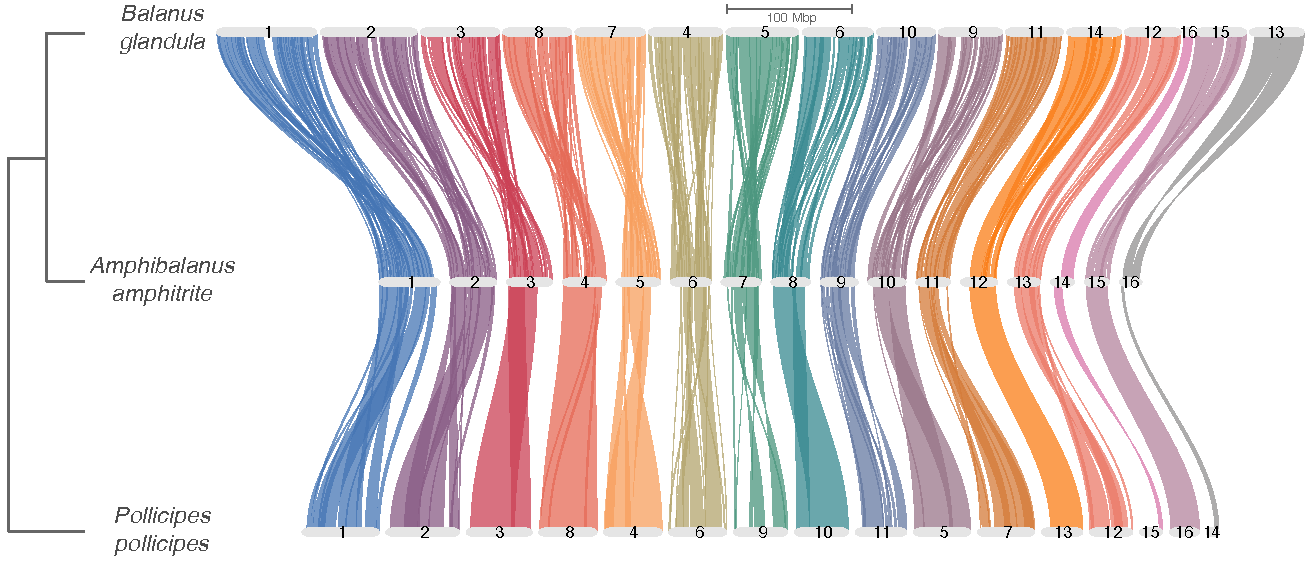
\includegraphics[width=0.95\textwidth]{figures/synteny.pdf}
    \caption{\textbf{Conserved synteny across barnacle genomes.}
        Genome-wide synteny plots showing one-to-one correspondence across
        16 putatively orthologous chromosomes between the genomes of \balgla{}
        (top), \textit{Amphibalanus amphitrite} (middle), and \textit{Pollicipes
        pollicipes} (bottom).
        Each colored line shows protein-coding orthologs across the three
        assemblies, colored according to their chromosome of origin in \bgla{}.
        Cladogram on the left shows the evolutionary relationship among the three
        species.}
    \label{fig:synteny}
\end{figure}

\subsection*{High genetic diversity in the \balgla{} reference assembly}

We estimated the genetic diversity present in the \bgla{} genome by identifying
heterozygous variants in our reference individual. After filtering low-quality sites
and masking regions with annotated repeats, we obtained genotypes for 314 million
sites along the genome, equivalent to 34.71\% of the 904.94\,Mbp present in the 58
scaffolds larger than 1\,Mbp (Table~\ref{tab:sup_popgen_stats}). Among these sites, 
9.08 million (2.89\%) were heterozygous in the reference individual, including 8.73
million SNPs and 356 thousand indels.
In total, this variation represents a mean density of 14.66 heterozygous sites per kbp
(median: 6 per kbp; standard deviation: 19.86).
Moreover, we observed nearly 400 thousand variant sites within protein-coding sequences,
including 144 thousand non-synonymous point mutations.
Transcripts in the reference individual had a mean of 7.74 (median: 3, standard
deviation: 14.97) non-synonymous heterozygous variants, indicating considerable coding
variation segregating within a single individual.
Even from this single genome, the sheer volume of heterozygosity underscores
the exceptionally large population sizes of this species and foreshadows
the extreme diversity observed at the population level.

\subsection*{Functional elements are conserved in barnacle genomes}

We used the \textsc{phastCons} package \citep{siepel_evolutionarily_2005} on the
\textsc{cactus} whole-genome alignment \citep{armstrong_progressive_2020} between
six barnacle species to identify highly conserved elements (HCE) in the Pacific
acorn barnacle genome.
Across the 16 putative chromosomes in the \textit{B. glandula} assembly, \textsc{phastCons}
identified 196{,}141 HCEs, spanning 50.85\,Mbp (6.05\%) of the 16 assembled chromosomes.
In \textit{B. glandula}, the HCEs had a mean length of 259.25\,bp (median: 42\,bp,
standard deviation: 990.40\,bp).
\vspace{0.1cm}

Following the identification of HCEs, we compared their sequence composition against
the genome-wide background (Figure~\ref{fig:phastcons}).
We first intersected the genomic coordinates of the HCEs with the \bgla{}
annotation, obtaining the proportion of annotated features among HCE sites
(Figure~\ref{fig:phastcons}A). Among our target features — which include an
``intergenic'' class for the unannotated fraction of the genome and a ``multiple''
class for overlapping features (e.g., a site spanning both a transposable element
and an intron) — all but one are present among HCEs. We did not observe any conserved
rRNA sites; however, this is likely the product of the whole-genome alignment, given
rRNA's repetitive nature and alignment difficulty \citep{gillespie_characterizing_2004},
and not an accurate measure of conservation (or lack thereof).
Aside from the absence of rRNAs, the sequence composition of HCEs largely followed that
of the whole genome.
Most annotated features do not appear substantially enriched among HCE sites
(Figure~\ref{fig:phastcons}B; Table~\ref{tab:sup_phastcons_enrichment}).
The two clear exceptions are coding sequences (CDSs) and tRNAs.
Protein-coding sequences display an approximately 2-fold enrichment among HCEs (mean
$\log_2$ enrichment: 0.75, median: 0.98, standard deviation: 0.93), reflecting the
conservation of protein-coding genes among barnacle genomes.
Similarly, tRNAs exhibit $\approx$4-fold enrichment in HCEs (mean $\log_2$ enrichment:
2.14, median: 2.04, standard deviation: 0.96), likely reflecting the strong functional
constraints on these sequences.
\vspace{0.1cm}

% Phastcons and enrichment
\begin{figure}[htbp]
    \centering
    \captionsetup{width=0.95\linewidth}
    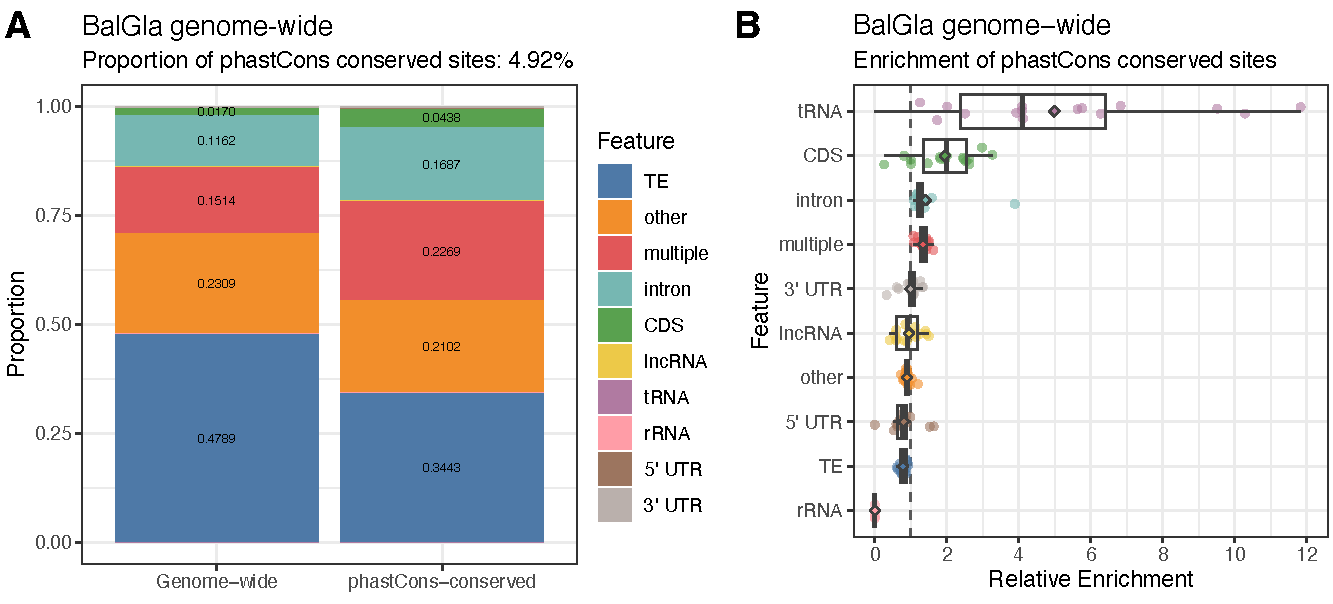
\includegraphics[width=0.9\textwidth]{figures/phastcons.pdf}
    \caption{\textbf{Highly conserved elements in the \balgla{} assembly.}
        \textbf{A.} Proportion of annotated features in the whole genome
        (left column) and the 50.85 Mbp spanning \textsc{phastCons}-conserved elements
        (right column). Values are shown only for elements with proportions larger than
        0.01. Sites that overlap more than one non-intergenic annotation type are
        represented by the ``multiple'' feature.
        \textbf{B.} Enrichment of the annotated features in the highly conserved
        elements compared to the genome-wide background, calculated as the $\log_2$ of
        the relative enrichment. The $\log_2$ enrichment values for each of the 16
        chromosomes are shown as points. The diamonds in the boxplot indicate the
        mean enrichment across the genome.}
    \label{fig:phastcons}
\end{figure}

The enrichment among conserved elements in \bgla{} mirrors patterns observed across other
groups of organisms.
First, coding sequences are consistently enriched among conserved elements, following the
patterns characterized by \citet{siepel_evolutionarily_2005} across vertebrate, insect, worm,
and yeast genomes.
While the raw composition of enriched conserved elements is different across all these
species, the consistent enrichment of CDSs is in accordance with the expectation that
protein-coding sequences are among the most functionally constrained genomic regions.
Secondly, the enrichment pattern in barnacles follows the same ordering observed across
both plants \citep{hupalo_conservation_2013} and animals \citep{siepel_evolutionarily_2005}:
tRNAs are the most enriched annotation among conserved regions, followed by CDSs, while
transposable elements are drastically underrepresented among HCEs.
In contrast, introns are mildly enriched among barnacle HCEs (Figure~\ref{fig:phastcons}B;
Table~\ref{tab:sup_phastcons_enrichment}), while depleted in plant
\citep{hupalo_conservation_2013}, insect, and vertebrate conserved elements
\citep{siepel_evolutionarily_2005}.
However, it remains unknown if this enrichment reflects the larger intronic fraction
of the barnacle genome or genuine intronic conservation in this lineage.
Overall, the conservation of functional elements across barnacle genomes indicates
that purifying selection has been effective at maintaining functionally constrained sequences
despite the highly repetitive nature of the genome, a pattern we revisit in the context
of the broader selective regime acting on these large populations.
% \vspace{0.1cm}

\subsection*{Patterns of molecular evolution reflect positive selection in protein-coding genes}

To examine the rate of molecular evolution in protein-coding sequences, we calculated
the pairwise ratio of non-synonymous to synonymous substitutions (\dnds) between
\bgla{} and its congener, the wrinkled barnacle \textit{Balanus crenatus},
using the codon counting approach described by~\citet{nei1986_dnds}.
We identified and aligned 9{,}082 single-copy orthologs between the two species.
The mean pairwise \dnds{} was 0.206 (median: 0.158, standard deviation: 0.191;
Figure~\ref{fig:sup_dnds}). This ratio indicates that, on average, coding
sequences in these barnacle genomes are under purifying selection, reflecting the
expected evolutionary constraints on sequences of functional importance.
\vspace{0.1cm}

Of the nine thousand genes assessed, 70 (0.77\%) displayed a \dnds{} $>$ 1, and are
likely candidates for positive selection.
The predicted function of the majority ($>80\%$) of these genes is unknown; however,
this is expected, since homology is likely harder to determine for fast-evolving
sequences putatively under strong selection.
Despite this limitation, we found several genes with known function among our positive
selection candidates, including a follistatin-A-like homolog, which is involved
in myogenesis and muscle development in crustaceans \citep{yan_identification_2021}.
We also observed a homolog of $\gamma$-interferon-inducible lysosomal thiol reductase,
which plays a role in crustacean innate immune response \citep{liu_involvement_2019}.
Additionally, we found evidence of positive selection in homologs of tumor protein
p53-inducible protein 11, which is involved in cell cycle regulation and is up-regulated
in crabs after viral infection \citep{cheng_p53_2021}, as well as a Quiver homolog, a
gene related to neuronal activity and sleep regulation in \textit{Drosophila}
\citep{wang_quiver_2010}.
\vspace{0.1cm}

We expanded on our \dnds{} measures of positive selection in protein-coding sequences
in the \bgla{} genome by incorporating population-level polymorphism using the
McDonald-Kreitman (MK) test \citep{mcdonald_adaptive_1991}.
Specifically, we used polymorphism data derived from a population panel of six \bgla{}
individuals from the central Oregon coast (see \nameref{sec:results_popgen}), comparing
those against the orthologous coding sequences in the \textit{B. crenatus} outgroup.
After removing alignments shorter than 100\,bp and those containing premature stop
codons and/or frameshift mutations, we calculated the MK test for 7{,}374 orthologous
sequences between \bgla{} and \textit{B. crenatus}.
\vspace{0.1cm}

Four hundred and forty-four (444, 6.02\%) of these orthologs showed a significant
deviation from the expected proportion of non-synonymous and synonymous substitutions
and polymorphisms (Figure~\ref{fig:mkTest}A).
We additionally calculated the Neutrality Index (NI;~\citealp{rand_excess_1996}) and
Direction of Selection (DoS;~\citealp{stoletzki_estimation_2011}) at each ortholog.
We observed a mean NI value of 0.745 (median: 0.554; standard deviation: 1.079) and
a mean DoS of 0.102 (median: 0.106; standard deviation: 0.131; Figure~\ref{fig:sup_dos}).
Both of these statistics (NI $<1$ and DoS $>0$) show that on average, and in contrast
with our measurements of \dnds{} (see \nameref{sec:discussion_dnds_mkt}), protein-coding
sequences in \bgla{} exhibit an excess of non-synonymous substitutions, suggesting that
they are evolving under positive directional selection when compared to the outgroup sequence.
Moreover, the near absence of genes displaying a significant excess in non-synonymous
polymorphism (NI $>1$) reflect a reduction the proportion of slightly deleterious
variants segregating in the population, suggesting the presence of highly efficacious
background selection.
\vspace{0.1cm}

In addition to NI and DoS, we calculated $\alpha$, a measure of the proportion
of non-synonymous substitutions fixed by positive selection \citep{smith_adaptive_2002}.
We calculated two adjusted versions of $\alpha$ to account for the presence of known
biases.
First, we calculated the Tarone-Greenland $\alpha$ estimator ($\alpha_\text{TG}$), a
weighted estimator that corrects for the effects of averaging over a large number of
genes \citep{stoletzki_estimation_2011}.
Across our 7{,}374 genes, we calculated an $\alpha_\text{TG}$ of 0.540 ($95\%$ CI:
0.534--0.550), which indicates that $\approx$ 54\% of non-synonymous substitutions in
this \bgla{} population were fixed as a product of positive selection.
Secondly, we calculated $\alpha$ using the asymptotic MK test ($\alpha_\text{asym}$),
which corrects for the presence of weakly deleterious non-synonymous polymorphisms
present at low frequency in the population \citep{messer_frequent_2013} which might
obscure the signal of positive selection.
We found a mean $\alpha_\text{asym}$ of 0.610 ($95\%$ CI: 0.610--0.622), a
larger proportion than that observed in \textit{Drosophila} ($\alpha_\text{asym} = 0.57$)
and humans ($\alpha_\text{asym} = 0.13$; \citealp{haller_asymptoticmk_2017,messer_frequent_2013}).
Regardless of the metric used, both $\alpha_\text{TG}$ and $\alpha_\text{asym}$ agree
that the majority of non-synonymous substitutions in this barnacle population are the
outcome of directional positive selection.
Notably, this pervasive signal of positive selection stands in apparent tension with
the low genome-wide \dnds{}, a discordance we address in the \nameref{sec:discussion}.
\vspace{0.1cm}

We explored the predicted function of the candidate genes under positive selection
identified in the MK test by performing a gene ontology (GO) enrichment analysis on the
367 candidates with available functional annotation.
The most enriched GO terms describe a coherent set of cellular functions, spanning the
plasma membrane, adherens junctions, myosin and spectrin complexes, and collagen trimers
(Figure~\ref{fig:mkTest}B;~Figure~\ref{fig:sup_go}).
Among the collagen-related terms, we additionally observe the enrichment of processes
related to the molting of arthropod cuticles (e.g., molting cycle, collagen and
cuticulin-based cuticle).
Together, these enrichment patterns suggest strong directional selection in \bgla{}
on genes involved in the building and remodeling of the cell surface, interactions with
the extracellular matrix, cell-cell adhesion, and related functions.
\vspace{0.1cm}

Several of our candidates under strong positive selection are direct components of these
enriched functions.
For example, two of our top candidates are non-muscle myosin heavy chain and myosin-VIIa homologs,
both showing a very large fraction of non-synonymous substitutions fixed by positive selection,
$\alpha$ of 0.961 and 0.940, respectively.
There is additional evidence of positive selection on proteins with known direct interactions,
such as the components of the spectrin heterodimer, spectrin $\beta$ chain ($\alpha = 0.898$) and
spectrin $\alpha$ chain ($\alpha = 0.895$), the integrin heterodimer, integrin $\alpha$
($\alpha$ = 0.793) and integrin $\beta$ ($\alpha = 0.810$), as well as non-muscle myosin heavy
chain ($\alpha = 0.961$; seen above) and its direct activator Rho-associated protein kinase 1
(ROCK1;~$\alpha = 0.939$).
Observing evidence of positive selection on interacting pairs is strongly suggestive of the
coevolution of these sequences, in a compensatory or correlated fashion; however, future research
is required to fully characterize the molecular interactions produced by these non-synonymous
substitutions in \bgla{}.
\vspace{0.1cm}

Outside of this cell remodeling and adhesion core, the remaining candidates of selection
appear largely functionally heterogeneous, spanning protein synthesis, osmoregulation,
and development (e.g., homologs of eukaryotic translation initiation factor 3 subunits
L and B, transmembrane channel-like 7, and patched domain-containing protein 3-like,
all with $\alpha > 0.9$; \citealp{lee_eif3_2015,liu_osmoregulatory_2025,bolatto_spatial_2015}).
Of these candidates, only a single significant gene in the MK test also appears among our
candidates of selection in the \dnds{} analysis --- a putative homolog of formin-like
protein 3, a member of a family of proteins known to play a role in crustacean immunity
\citep{li_formin-like_2025} --- further highlighting the discrepancy between the two
tests of selection.
Finally, our single candidate showing a significant excess of polymorphism relative to
divergence is a homolog of tubulin $\alpha$-1C chain-like, a major constituent of
microtubules and thus directly linked to the cell-remodeling machinery under positive
selection.
The large excess of polymorphism at this gene (NI = 18.54) instead suggests balancing
selection, and this homolog has additionally been observed as differentially expressed
in response to osmotic stress in barnacles \citep{chandramouli_transcriptome_2015}.

% MK test volcano plot
\begin{figure}[htbp]
    \centering
    \captionsetup{width=0.95\linewidth}
    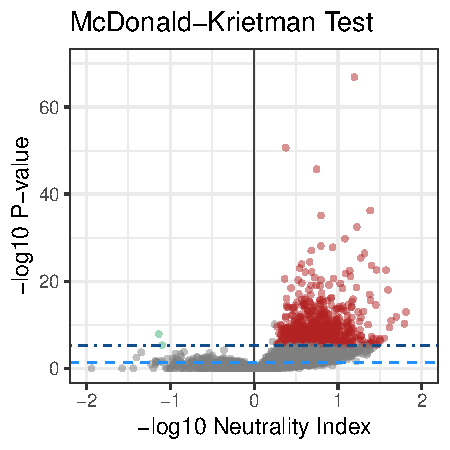
\includegraphics[width=0.95\textwidth]{figures/mkTest.pdf}
    \caption{\textbf{Signatures of positive selection in \balgla{}
        protein-coding genes.}
        \textbf{A.} Selection on 7{,}374 protein-coding genes was assessed using the
        McDonald-Kreitman test.
        X-axis denotes the $-\log_{10}$ of the Neutrality Index, with values on the
        right (NI $<1$) indicating excess of non-synonymous substitutions indicative of
        positive selection.
        Y-axis denotes the $-\log_{10}$ $p$-value of the McDonald-Kreitman test.
        The dashed and dot-dashed lines show the raw ($p<0.05$) and Bonferroni-corrected
        ($p<6.20\times10^{-6}$) significance thresholds, respectively.
        Points in red show the 444 candidates under positive selection, genes with a
        significant excess of fixed non-synonymous substitutions.
        Point in green show the one significant gene with an excess of non-synonymous
        polymorphism.
        \textbf{B.} Significant GO term enrichment among the candidates under
        positive selection in the McDonald-Kreitman test.
        $p_\text{elim}$ denotes the $p$-value calculated from \textsc{topGO}'s
        \texttt{elim} algorithm \citep{alexa_topgo_2006}, which accounts for redundancy
        among GO terms.
        Top, middle, and bottom panels show the top four terms with the largest
        enrichment among the candidates under selection for the three GO categories:
        biological processes, cellular component, and molecular function.}
    \label{fig:mkTest}
\end{figure}

\subsection*{Barnacle genes show biases in the use of synonymous codons}

We compared biases in the usage and composition of synonymous codons in 12 metazoan
genomes, including four barnacles (Table~\ref{tab:sup_enc_summary}), to study the effects of
translational selection in the context of large populations.
Using the annotated transcript sequences in these genomes we calculated the effective number
of codons (ENC), a measure of the extent of departure from equal usage across synonymous
codons \citep{wright_effective_1990,sun_improved_2013}.
In addition to ENC, we also estimated compositional biases by calculating both the overall
coding sequence GC proportion, and the proportion of GC bases at third codon positions (GC3s).
Across 16{,}217 genes in \bgla{}, we find a mean ENC of 43.17 (median: 42.84, standard
deviation: 5.52; Figure~\ref{fig:codon_enc}A;~Table~\ref{tab:sup_enc_summary}).
This number of effective codons is similar to the one observed across three other barnacle
genomes (mean ENC ranging from 42.04 to 44.33; Table~\ref{tab:sup_enc_summary}), highlighting a
substantial reduction in the number of synonymous codon used in barnacles when compared to other
metazoans (Figure~\ref{fig:codon_enc}A).
A similar trend is observed when compared nucleotide composition in barnacle coding sequences
when compared to other metazoans.
All four barnacle genomes studied showed coding sequence GC content of $\approx64\%$, 10 to 20\%
higher than the other studied genomes (Figure~\ref{fig:codon_enc}B;~Table~\ref{tab:sup_enc_summary}).
The higher coding GC proportion in barnacles is also observed when looking at the GC proportion
at 3rd codon positions and at 4-fold degenerate sites (Figure~\ref{fig:sup_coding_gc}).
\vspace{0.1cm}

We explored the selective basis of the increased bias in codon usage in barnacle genomes by
comparing the empirical ENC distribution against a theoretical expectation.
In its original definition of the ENC statistic, \citet{wright_effective_1990} devised a
relationship between GC3s and ENC, resulting in an expected number of effective codons for a
given GC content.
Deviations from this expectation, specifically observing a smaller number of effective codons
than expected, suggest the presence of strong translational selection acting on the genome.
After testing this relationship across these 12 genomes, we observe that the reduction in
the number of effective codons observed in barnacles can in most cases be explained by their
coding GC proportion (Figure~\ref{fig:sup_enc_gc3s}; Figure~\ref{fig:sup_enc_reg}), suggesting
a codon usage bias driven by neutral processes.
In \bgla{} specifically, we observed a moderate deviation when comparing the empirical ENC
distribution against Wright's curve (Figure~\ref{fig:codon_enc}C); however, when comparing the
linear relationship between observed and expected ENC, a better fit for GC biased genomes such
as \bgla{}, we do observe a reduction in the model's slope and coefficient of determination
($\text{R}^2$; Figure~\ref{fig:codon_enc}D).
This poorer fit of the model indicates a smaller than expected number of effective codons, and
suggests the presence of strong translational selection acting on the genome and the potential
non-neutrality of at least some synonymous codons in large \bgla{} populations.
\vspace{0.1cm}

Comparing the ENC and GC3s distribution in relation to population size highlights some
interesting patterns.
Evidence for selection-driven codon usage biases is observed for some hyper-diverse, large
population species, e.g., the nematode \textit{Caenorhabditis brenneri}, the Pacific oyster
\textit{Magallana gigas}, and the European lancelet \textit{Branchiostoma lanceolatum}
(Figure~\ref{fig:sup_enc_gc3s}; Figure~\ref{fig:sup_enc_reg}; Table~\ref{tab:sup_enc_models}).
More moderate deviation is observed for other diverse species, e.g, the malaria mosquito
\textit{Anopheles gambiae} and the tunicate \textit{Ciona intestinalis}.
In contrast, in three of our studied barnacles (\textit{B. crenatus}, \textit{A. amphitrite},
and \textit{P. pollicipes}), the observed codon usage biases appear are indistinguishable from
neutral compositional processes.
In \bgla{}, evidence for non-neutral codon usage biases is moderate to strong depending on the
method used.
Overall, while we do not observe a clear relationship between population size and codon usage
biases in the 12 studied genomes, the lineage-specific patterns described here provide an
unexplored avenue of study of the efficacy and breadth of selection in highly diverse genomes.

% ENC codon bias
\begin{figure}[htbp]
    \centering
    \captionsetup{width=0.95\linewidth}
    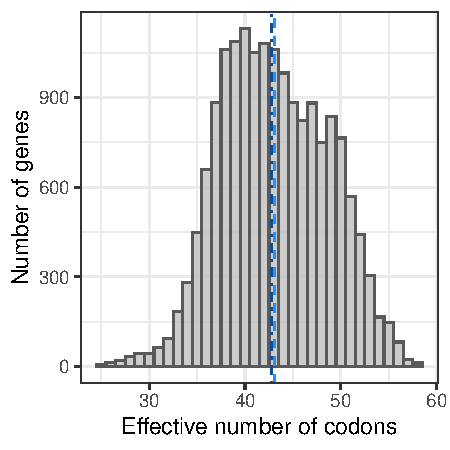
\includegraphics[width=0.9\textwidth]{figures/codon_bias.pdf}
    \caption{\textbf{Codon usage biases in \balgla.}
        \textbf{A.} Genome-wide distribution of the effective number of codons (ENC)
        in \bgla{} (\texttt{BalGla}) and other metazoan genomes (see Table~\ref{tab:sup_enc_summary}),
        including the barnacles \textit{B. crenatus} (\texttt{BalCre}), \textit{A. amphitrite}
        (\texttt{AmpAmp}), and \textit{P. pollicipes} (\texttt{PolPol}).
        The vertical lines show the 50\textsuperscript{th} quantile (median) of the
        distribution, while the crosses show the mean value.
        \textbf{B.} Distribution in the proportion of GC bases in coding sequences
        of 12 metazoan genomes. Vertical lines and crosses show the mean and median
        values, respectively.
        \textbf{C.} Relationship between the GC proportion at the 3rd codon site (GC3s)
        and ENC in \bgla{}. Each black dot represents a gene, while the red curve shows
        the expected relationship in accordance with Wright's curve
        \citep{wright_effective_1990}. Points below the curve show genes with a smaller
        than expected number of effective codons, candidates for translational selection.
        \textbf{D.} Relationship between the expected number of effective codons (according
        to Wright's curve) and the empirical ENC distribution in \bgla{}. Red line shows the
        linear regression between expected and observed ENC distributions.}
    \label{fig:codon_enc}
\end{figure}

\subsection*{Barnacle populations exhibit elevated genetic polymorphism}\label{sec:results_popgen}

We sequenced the whole genomes of eight \bgla{} individuals from the central Oregon coast
using Illumina short reads.
After removal of two samples with poor quality sequences, and the stringent filtering of
sites with low coverage, low quality, and/or missing genotypes, we recovered a total of
111.6 million genotyped sites (Table~\ref{tab:sup_popgen_stats}), 21.4 million (19.16\%)
of which were variant in the six retained samples.
Among these variant sites, we recovered 20.5 million point mutations, 4.86\% of which 
were multiallelic in just these six individuals.
In total, the amount of polymorphism observed in our sampling translates to a mean
density of 41.1 variant sites per kbp (median: 29, standard deviation: 40.82).
Moreover, 1.1 million of these variant sites (5.23\%) were located in coding sequences.
These coding variants included 360 thousand missense (non-synonymous) mutations,
corresponding to a mean of 18.93 non-synonymous variants per transcript
(median: 10, standard deviation: 28.50).
Overall, these represent a substantial proportion of coding variation segregating in
central Oregon.
This \bgla{} population displayed a mean genome-wide nucleotide
diversity ($\pi$) of 0.0506 (median: 0.0531, standard deviation: 0.0188;
Figure~\ref{fig:genome_pi}; Table~\ref{tab:sup_feature_pi}).
For context, this magnitude of $\pi$ is approximately $4\times$ higher than that
observed in \textit{Anopheles gambiae} mosquitos, a species known for their high
levels of polymorphism, $\approx7\times$ higher than the diversity in Sub-Saharan
populations of \textit{Drosophila melanogaster}, and $\approx48\times$ higher than the
diversity observed in large human cohorts~(Figure~\ref{fig:sup_pi_comp}).
\vspace{0.1cm}

Along each chromosome, we did not observe any strong correlation between the density
of specific genomic features (e.g., CDSs, lncRNAs, tRNAs, introns, and repeats) and
$\pi$, particularly not at the scale of 10\,kbp (Figure~\ref{fig:genome_pi};
Figure~\ref{fig:sup_pi_pairplot}).
However, stronger relationships are likely present at other genomic intervals given
the differences in diversity seen across genetic elements (see below).
The strongest correlation was, expectedly, observed between the density of segregating sites
within 10\,kbp windows and $\pi$ (Spearman's $\rho$: 0.706; Figure~\ref{fig:sup_pi_pairplot}).
The proportion of segregating sites in itself was not correlated with the density of
particular genomic features, except for repeats; however, this is likely an artifact of the
masking of genotypes located within repetitive intervals in the reference
(see \nameref{sec:methods_popgen}).
Despite the lack of clear correlation, the patterns of $\pi$ observed along
the chromosomes are qualitatively similar to those expected under regimes of
strong linked selection, in which regions of reduced diversity are the result
of differences in the recombination landscape (e.g., reduction in recombination
in centromeric regions).
Describing recombination in detail this species should thus be a focus of future studies
in order to characterize how highly efficacious selection and linkage shape genetic
diversity along the genome in \bgla{}.
\vspace{0.1cm}

% Genome-wide pi & repeat and gene density
\begin{figure}[htbp]
    \centering
    \captionsetup{width=0.95\linewidth}
    \includegraphics[width=1.0\textwidth]{figures/genome_pi.pdf}
    \caption{\textbf{Nucleotide diversity ($\pi$) and coding and repeat density
        along the \balgla{} genome.}
        \textbf{A.} Density of coding sequences (CDS) along the genome, defined as the
        proportion of bases annotated as CDS within 10\,kbp windows. Line reflects the
        kernel-smoothed values along a 1\,Mbp window. Dashed horizontal line shows
        the genome-wide average proportion of CDS bases (0.0288). Top and bottom
        horizontal axes show the chromosome number and genomic position, respectively.
        \textbf{B.} Density of repeat elements annotated within 10\,kbp windows, smoothed
        along 1\,Mbp intervals. Dashed horizontal line shows the genome-wide average
        proportion of repeat bases (0.597).
        \textbf{C.} Density of segregating sites, calculated as the proportion of SNPs
        within 10\,kbp windows, smoothed along 1\,Mbp intervals. Dashed horizontal line
        shows the genome-wide average proportion of segregating SNPs per 10\,kbp
        (0.0307).
        \textbf{D.} $\pi$ within 10\,kbp windows, smoothed along 1\,Mbp intervals.
        Horizontal dashed line shows the mean genome-wide $\pi$ (0.0506).}
    \label{fig:genome_pi}
\end{figure}

Looking at diversity across the genome, we observed an overall reduction in $\pi$
at putatively functional sites. For example, the mean $\pi$ in sequences spanning
annotated CDSs is 0.0302 (median: 0.0270, standard deviation: 0.0221;
Figure~\ref{fig:feature_pi}; Table~\ref{tab:sup_feature_pi}),
which represents a $\approx1.6\times$ reduction in diversity when compared to the
genome-wide average. A reduction in diversity of similar magnitude is also observed
in the sequences of lncRNAs ($1.4\times$) and 5' UTRs ($1.3\times$). The largest reduction
in diversity when compared to the genome-wide background was observed in tRNAs, with
$\pi~\approx4.3\times$ lower than the genomic background and consistent with the
strong functional constraint evidenced by their enrichment in highly conserved elements.
In contrast to most other elements of the genome, introns display a relative increase in
diversity, with a mean $\pi$ of 0.0646 (median: 0.0650, standard deviation: 0.0299),
approximately $1.3\times$ higher than the genome-wide average.
\vspace{0.1cm}

Zooming in further on coding sequences, we explored the patterns of $\pi$
at 0-fold degenerate ($\pi_{0}$), in which any mutation produces a non-synonymous
substitution, and 4-fold degenerate sites ($\pi_{4}$), in which any mutation results
in a synonymous change.
This comparison allows us to compare diversity at constrained versus neutral (or
putatively neutral) sites.
In this central Oregon population of \bgla{}, the mean $\pi_{0}$, was 0.0107 (median:
0.00292, standard deviation: 0.0178).
This is the lowest diversity among the studied categories in the genome, not a
surprising result given the higher functional constraint expected at these sites.
In contrast, mean $\pi_{4}$ was 0.0790 (median: 0.0750, standard deviation: 0.0483),
$\approx1.6\times$ higher than the genome-wide average and the highest in the genome.
The nearly 8-fold difference between $\pi_{0}$ and $\pi_{4}$ highlights the
strong constraint on non-synonymous sites and suggests that purifying selection is
highly effective in this population, consistent with theoretical predictions for
species with large effective population sizes.

% Distribution of pi for different features in the genome
\begin{figure}[htbp]
    \centering
    \captionsetup{width=0.95\linewidth}
    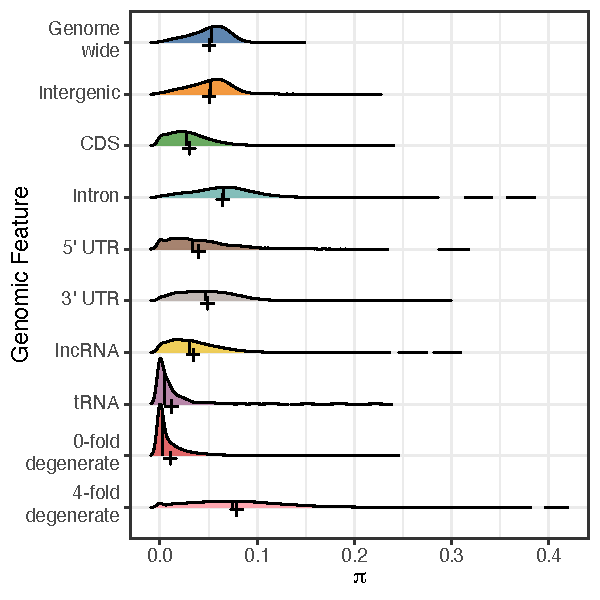
\includegraphics[width=0.6\textwidth]{figures/feature_pi.pdf}
    \caption{\textbf{Nucleotide diversity ($\pi$) across genomic
        features in Oregon \balgla.}
        The density histogram shows the distribution of windowed
        $\pi$ values across different genomic features annotated
        in the \bgla{} assembly. The vertical lines show the
        50\textsuperscript{th} quantile (median) of the distribution,
        while the crosses show the mean value.}
    \label{fig:feature_pi}
\end{figure}

\subsection*{\balgla{} exhibits large effective population sizes}

We estimated the effective population size (\Ne{}) for a central
Oregon \textit{B. glandula} population sample using the whole-genome genotypes.
As a simple estimate of the long-term \Ne{} of this population, we first
calculated \Ne{} using Watterson's estimator of genetic diversity ($\theta_\text{W}$),
observing a mean genome-wide $\theta_\text{W}$ of 0.0617 (median: 0.0635, standard
deviation: 0.0224; Figure~\ref{fig:sup_theta_ne}). Assuming a per-base,
per-generation mutation rate ($\mu$) of $3\times10^{-9}$ (as estimated by
\cite{nunez_footprints_2020} for the northern acorn barnacle \textit{S. balanoides})
and using the relationship between \Ne{} and $\theta_\text{W}$, this yields a
mean effective size of 5{,}137{,}172 (median: 5{,}289{,}211, standard deviation:
1{,}862{,}683), which is consistent with the expectation of large \Ne{} in this species.
\vspace{0.1cm}

Additionally, we estimated \Ne{} through time using a coalescent-based
approach with \textsc{msmc2} \citep{dutheil_msmc_2020}. This estimate also placed
the historical effective size of the population on the order of $10^{6}$ individuals
(between $10^{6}$ and $10^{7}$ generations ago) (Figure~\ref{fig:sup_mcmc_ne});
however, given our small sample size and the use of only within sample pairwise
comparisons, we were unable to obtain accurate \Ne{} estimates at more recent
($<10^{5}$ generations) timescales using \textsc{msmc2}.
Nevertheless, even these conservative estimates place \bgla{} among the
largest known effective population sizes for any eukaryote, yet orders of
magnitude below the census sizes observed in the field --- a disparity
central to Lewontin's Paradox and one we return to in the Discussion.

\section*{Discussion}\label{sec:discussion}

\commentauth{Angel}{From Scott's comment, maybe we remove the first section
altogther (or 1 paragraph at most?). We use that space to move some of the allozyme
discussion here. Andy notes: We leave this here now and wait for review.}

\subsection*{Genome assembly in highly polymorphic species}

Improvements in the affordability, accessibility, and accuracy in sequencing
technologies have increased the generation of high quality reference genomes across
the tree of life. Over the last decade, we have seen the research outcomes of large
genome assembly consortiums, e.g., the Vertebrate Genome Project
\citep{rhie_towards_2021} and the Earth BioGenome Project
\citep{blaxter_earth_2025}, tackling the production of high quality genomes across
diverse taxa. We have also seen the generation of complete genomes, sequencing
whole chromosomes at a telomere-to-telomere scale \citep{nurk_complete_2022,
yoo_complete_2025}, as well as the sequencing and assembly of some of the largest
and most repetitive genomes known in nature \citep{campos-dominguez_genome_2025}.
Best practice protocols have also become available to applying these methods to new
taxa in a reproducible fashion \citep{lawniczak_best-practice_2025,li_genome_2024}.
\vspace{0.2cm}

Despite these advances, there appears to be a gap in knowledge in the analysis of
highly polymorphic organisms, such as barnacles. High heterozygosity presents
problems during the assembly process, e.g., hindering the differentiation between
paralogs and haplotypes, which often results in the inflation of the genome size and
a high proportion of duplicated sequences \citep{guiglielmoni_phasing_2024,
asalone_regional_2020,roach_purge_2018,mochizuki_practical_2023}. The most common
approach is to manage these haplotypes \textit{a posteriori}, purging them after
initial assembly \citep{guan_identifying_2020,roach_purge_2018}; however, while this
approach can be successful in generating haploid assemblies, as we have shown here,
it is not without its drawbacks. First, purging haplotypes could lead to a reduction
in the gene completeness in the main assembly, as primary haplotypes might be
incorrectly labelled as haplotigs, leading to their removal. Secondly, the ability
to identify and remove haplotypes is dependent on the properties of the assembly.
Sequences that are too fragmented and/or too divergent from one another are likely
harder to purge due to difficulties in mapping. Moreover, when performing phased
diploid assemblies, the excessive presence of haplotypes will interfere with
phasing, leading to a main haploid assembly that is a mosaic between the two
haplotypes and/or the poor quality of the secondary assembly.
\vspace{0.2cm}

These difficulties drive the need for the development of methods and analysis
best-practices focused on the assembly of highly heterozygous genomes, and for a
further exploration of how elevated heterozygosity affects \textit{de novo} assembly
parameters.
In particular, the assembly of phased diploid genomes has seen several improvements
in recent years, e.g.,
the direct purging of haplotigs and the integration of Hi-C data to phase haplotypes
without the need of parental genotypes in \textsc{hifiasm}
\citep{cheng_haplotype-resolved_2022},
and the integration of Hi-C and ultra-long read data for phased telomere-to-telomere
haplotypes in \textsc{Verkko2} \citep{antipov_verkko2_2025}.
Yet, it is presently unknown if these new methods are all equally suitable for highly
heterozygous genomes and further work is likely needed before we can obtain
haplotype-resolved genome assemblies for hyperpolymorphic organisms.
Despite these limitations, our work here, assembling a chromosome-level assembly for
a heterozygous barnacle species --- even if not fully phased --- is a step in the
right direction of generating high-quality genomic resources for these
highly diverse and difficult genomes.

\subsection*{Genome evolution in large populations}

Evolutionary processes at large demographic scales are expected to leave distinct
signatures in the genome, several of which are observed in our Pacific acorn
barnacle assembly.
For example, large populations are expected to harbor increased levels of segregating
polymorphism, the product of both the reduction in the stochastic loss due to
genetic drift and the increase in the population-scale mutation rate.
In accordance, we observe a barnacle genome with extreme levels of genetic diversity,
both at the individual and population level (Figure~\ref{fig:sup_kmers};
Table~\ref{tab:sup_popgen_stats}), a substantial proportion of which is located in
coding sequences.
\vspace{0.2cm}

Similarly, large populations experience an increase in the efficacy of purifying
selection, which is expected to reduce the levels of diversity and increase 
conservation across functional sequences.
We see these patterns reflected in the \bgla{} genome.
Putatively functional sites, particularly coding exons and tRNAs, show both increased
levels of sequence conservation (Figure~\ref{fig:phastcons}) and a reduction in
population-level genetic diversity (Figure~\ref{fig:feature_pi};
Table~\ref{tab:sup_feature_pi}) compared to less constrained features of the genome.
Notably, the rank ordering of the enrichment of conserved elements, with tRNAs and CDSs
as the most enriched, parallels findings in insects \citep{siepel_evolutionarily_2005},
suggesting that the targets of purifying selection are broadly conserved across
arthropods despite the much larger and more repeat-rich genome of \bgla{}.
Increased efficacy of purifying selection is also reflected in the results of the
McDonald-Kreitman test (Figure~\ref{fig:mkTest}), where we observe a relative decrease
in the proportion of non-synonymous polymorphism in a central Oregon \bgla{} population,
suggesting that weakly deleterious variants are more efficiently purged by selection
\citep{li_reverse_2008}.
Positive selection is also expected to increase in efficacy in large populations,
resulting in the fixation of a larger fraction of beneficial non-synonymous mutations.
We observe this pattern as well: in this central Oregon population, the majority
(54 to 61\%, depending on the metric of $\alpha$ used) of non-synonymous substitutions
reached fixation due to positive selection, a proportion higher than that observed in
diverse \textit{Drosophila} populations \citep{haller_asymptoticmk_2017}.
\vspace{0.2cm}

In large enough populations, selection should be efficacious enough that its effects
extend to synonymous sites, where substitutions are normally considered neutral.
This could result in a bias in the usage of synonymous codons, as different codons are
favored over others due to GC biases, tRNA abundance, and other factors
\citep{galtier_codon_2018}.
These effects are observed in the \bgla{} assembly in the form of reduction in the
effective number of codons seen across protein-coding genes (Figure~\ref{fig:codon_enc}).
On average, \bgla{} uses $\approx$ 43 out of 61 available codons, a greater reduction
than that observed in \textit{D. melanogaster} (Figure~\ref{fig:sup_dmel_enc}).
This strong bias in codon usage further reflects an increase in the efficacy of natural
selection due to the large size of Pacific acorn barnacle populations.
Moreover, these biases put into question the neutrality of at least some synonymous
substitutions in this system, which could have important ramifications for the study of
molecular evolution; however, the extent of these effects remain presently unknown and
should be the subject of future study.
\vspace{0.2cm}

In contrast, the distribution of transposable and repeat elements in the
\bgla{} assembly was unexpected, as we find a highly repetitive genome
composed of over 60\% repeats (Figure~\ref{fig:genome_pi};
Table~\ref{tab:sup_earlgrey_summary}).
Previous work has shown that purifying selection plays a key role in the accumulation
and fixation of transposable elements \citep{merel_relaxed_2025,langmuller_genomic_2023,
bourque_ten_2018}, following the expectation that repetitive sequences are, on average,
slightly deleterious.
Given the increased efficacy of selection we observed in the rest of the genome,
our expectation was to find a relatively small proportion of repeats.
However, the high repeat content observed in the genome does not necessarily
reflect the low efficacy of selection in these populations.
Some could be low-frequency, slightly deleterious variants in the process of being purged
from the population.
Other repeats might represent beneficial genetic variation, as transposable elements are
known to play roles in adaptive evolution \citep{schrader_impact_2019}.
For example, repeat elements can act as regulators of gene expression
\citep{trizzino_transposable_2017,rech_population-scale_2022}, and as such may provide
the regulatory plasticity required for survival in rapidly changing
intertidal environments.
Regardless of their role, disentangling the population-wide repeat landscape and its
fitness effects is likely impossible with a single haploid reference assembly.
Thus, this observation drives the need for larger comparative genomic studies across
barnacle populations before we can fully understand the dynamics of genomic repeats
and transposable elements in this and other large populations.

\subsection*{Molecular evolution in large populations: reconciling \dnds{} and the
McDonald-Kreitman test}\label{sec:discussion_dnds_mkt}

One of the more striking patterns in our results is the apparent discordance between
our two measures of selection on protein-coding genes.
The average pairwise \dnds{} between \bgla{} and \textit{B. crenatus} is 0.206,
indicating that the majority of coding sites are under purifying selection.
Yet the McDonald-Kreitman test reveals a seemingly opposite pattern: $\approx61\%$
of non-synonymous substitutions fixed between these species were driven by
positive selection ($\alpha_\text{asym}$ = 0.610).
At first glance, these results appear contradictory: how can coding sequences be
under strong purifying selection while simultaneously showing pervasive adaptive
evolution?
\vspace{0.2cm}

The resolution lies in the fact that \dnds{} and the McDonald-Kreitman test measure
fundamentally different quantities. The \dnds{} ratio averages across all
non-synonymous sites in a gene, the vast majority of which are under functional
constraint, resulting in a ratio well below one. In contrast, the McDonald-Kreitman
test partitions changes into polymorphism and divergence, using synonymous changes
as a neutral baseline to ask whether there is an \textit{excess} of non-synonymous
fixations relative to the neutral expectation. This test is therefore sensitive to
the subset of non-synonymous mutations that escape purifying selection and reach
fixation, even when most non-synonymous sites in a gene are constrained.
Moreover, pairwise \dnds{} is calculated from a single sequence per species and
therefore incorporates segregating polymorphisms into its divergence estimate. In
species with many weakly deleterious non-synonymous variants segregating at
appreciable frequencies, this can inflate the non-synonymous divergence and distort
estimates of selection \citep{li_reverse_2008}. By explicitly separating
polymorphism from fixation, the McDonald-Kreitman test avoids this conflation.
\vspace{0.2cm}

\cite{li_reverse_2008} compared the performance of \dnds{} and the McDonald-Kreitman
test across human, \textit{Drosophila}, and yeast genomes and found that the two
approaches identify distinct but correlated sets of genes as targets of selection.
Notably, the McDonald-Kreitman test was more powerful than \dnds{} only in
\textit{Drosophila}, the species with the highest polymorphism, where it
identified nearly three times as many genes under positive selection. In the
lower-diversity human and yeast datasets, the pattern was reversed. This finding
suggests that the statistical power of the McDonald-Kreitman test is greatest in
high-polymorphism species, making it particularly well suited for systems like
barnacles where segregating variation is abundant.
\vspace{0.2cm}

The pattern we observe in \bgla{} is thus consistent with theoretical expectations
for large populations: strong purifying selection efficiently removes the majority
of deleterious non-synonymous mutations, keeping \dnds{} low, while at the same time
the increased efficacy of positive selection drives a disproportionate fraction of
the remaining non-synonymous substitutions to fixation, producing a high
$\alpha$. This coupling of strong purifying and positive selection is a hallmark
of evolution in large populations and has been observed in \textit{Drosophila}, where
$\alpha_\text{asym}$ is approximately 0.57 \citep{messer_frequent_2013}.
Our estimate of $\alpha_\text{asym}$ of 0.610 in \bgla{} is comparable to
or slightly higher than that in \textit{Drosophila}, consistent with the expectation
that the even larger effective population size in barnacles further increases the
efficacy of both modes of selection.
\vspace{0.2cm}

A locus-level example of this complementarity between tests emerges at the malic
enzyme paralogs: the MK test flags \textit{Me.2} through an excess of
non-synonymous fixations ($\alpha = 0.719$), the signature of recurrent positive
selection, while the classic HKA test flags \textit{Me.1} --- albeit at nominal
significance ($p = 0.032$, uncorrected) --- through a deficit of silent polymorphism
relative to divergence, the signature of a recent selective sweep at linked neutral
sites. That the two paralogs are detected by different tests underscores that the
tempo and mode of adaptive evolution can differ substantially even between close copies
of the same gene.
Because the two copies of NADP-dependent malic enzyme share deep sequence homology but
differ in genomic context, this paralog-level asymmetry cautions against treating
classical ``allozyme loci'' as monolithic units in genome-scale reanalyses.
\vspace{0.2cm}

The \textit{Gpi} result provides a second connection between our genome-wide analyses and
the allozyme literature.
\cite{hedgecock_temporal_1994} identified \textit{Gpi} as one of several \bgla{} loci
showing significant microgeographic heterogeneity in allele frequencies, but allozyme-era
methods could not distinguish whether that heterogeneity reflected protein-level
selection, drift, or chaotic recruitment among sweepstakes-limited larval cohorts
\citep{hedgecock_does_1994}.
Our sequence-level data now show that \textit{Gpi} in \bgla{} has accumulated a
substantial excess of non-synonymous fixations relative to the neutral expectation,
consistent with a history of directional positive selection on the protein itself.
This pattern contrasts with prior work at the \textit{Gpi} ortholog in
\textit{S. balanoides}, where the MK test has not yielded a comparable signal
\citep{nunez_footprints_2020,rand_ecological_2002} --- illustrating that ``same allozyme
locus'' comparisons across congeneric barnacles can obscure real divergence in
selective history.
\textit{Gpi} encodes a glycolytic enzyme at the branch point between glycolysis and the
pentose phosphate pathway; protein-coding variation at \textit{Gpi} in other marine
invertebrates has been linked to thermal tolerance and metabolic flux under osmotic and
thermal stress \citep{flight_allozyme_2012}, providing a plausible functional axis along
which directional selection could act in Pacific intertidal populations.
\vspace{0.2cm}

At \textit{Mpi}, the modest excess of non-synonymous polymorphism (NI $>$ 1) is
suggestive of --- but does not establish --- a regime of balancing selection.
\cite{hedgecock_temporal_1994} documented significant allele-frequency heterogeneity at
\textit{Mpi} across a 1-m intertidal transect at Bodega Harbor, a pattern analogous to
that subsequently documented at the \textit{Mpi} ortholog in \textit{S. balanoides}
\citep{nunez_footprints_2020,rand_ecological_2002}, where alternative alleles are
beneficial at different intertidal habitats.
However, intertidal microhabitat is approximately uniform in our central Oregon sampling,
so we cannot directly test the habitat-based balancing-selection hypothesis developed in
\textit{S. balanoides}.
Future sampling of \bgla{} across its geographic range and across intertidal
microhabitats will be needed to determine whether balancing selection at \textit{Mpi} is
shared across these systems or reflects distinct evolutionary histories in Atlantic and
Pacific barnacles.

\subsection*{Barnacles as models for evolution at biological extremes}

Our work shows that a Pacific acorn barnacle population from central Oregon exhibits
genetic diversity of over 5\% (mean genome-wide $\pi$ of 0.0506).
These levels of genetic diversity are higher than those observed for other model
systems known for their relatively large population sizes.
For example, the genome-wide $\pi$ we observe in this population is an order of
magnitude higher than that observed in \textit{Drosophila} (Figure~\ref{fig:sup_dmel_pi})
\citep{nunez_footprints_2025,li_comparative_2025,pool_population_2012,
langley_genomic_2012}.
Even the $\pi$ observed at 0-fold degenerate sites, the least diverse and among the
most constrained sites in the genome, is still an order of magnitude higher than the
diversity observed genome-wide in these \textit{Drosophila} populations.
While elevated, this level of diversity is not unique to barnacles.
Similar magnitudes of genome-wide $\pi$ ($\approx10^{-2}$) have been observed
in other taxa, including corals \citep{meziere_corals_2025}, parasitic nematodes
\citep{stevens_nematodes_2023}, bivalves \citep{liu_bivalves_2025}, and mosquitoes
\citep{kent_aedes_2025,ag1000g}.
Moreover, as with other marine invertebrates, barnacle life history traits are likely
direct drivers of the elevated polymorphism observed, as factors such as large census
sizes, small propagule size, long larval dispersal, and broad geographic distribution
have been positively correlated with high genetic diversity in these
organisms \citep{leffler_revisiting_2012,romiguier_comparative_2014}.
\vspace{0.2cm}

The magnitude of diversity observed in \bgla{} solidly places them among
hyperpolymorphic populations, those exhibiting diversity above 5\%
\citep{cutter_molecular_2013}. This adds barnacles to a growing list of emerging
hyperpolymorphic model systems, which are key to studying the limits of biological
variation and molecular evolution in natural populations. Moreover, our observations
of extreme genetic diversity also have important implications for the study of species
boundaries. For example, recent work by~\cite{hart_genomic_2025} suggests that levels
of above 1\% neutral diversity in Eukaryotes likely serve as biological limits for the
definition of species. Barnacles and other hyperpolymorphic populations put these
putative cutoffs into question. We observe levels of genome-wide diversity of over 5\%
in just a very small portion of the biological range of the Pacific acorn barnacle.
Nucleotide diversity is even higher ($\approx8\%$) at 4-fold degenerate, and putatively
neutral, sites (Figure~\ref{fig:feature_pi}; Table~\ref{tab:sup_feature_pi}).
Given the species' broader geographical and ecological distribution, genetic
diversity is likely to increase when looking across the whole range. This
observation reiterates the importance of future studies of genetic diversity
of this species over its whole geographic range, providing some insights on
the mechanisms that maintain population and species boundaries in the presence
of extreme genetic diversity.
\vspace{0.2cm}

Beyond species boundaries, the extreme diversity observed in barnacles also speaks to
a long-standing question in population genetics: the relationship between effective
and census population sizes. From our results on diversity, we
observe that this barnacle population has an effective size of approximately $10^{6}$.
However, these populations also show densities of $10^{4}$ individuals per square meter
\citep{menge_recruitment_2000}. Based on this estimate, the census size of the Pacific
acorn barnacle population in central Oregon should be, conservatively, in the billions of
individuals. While the general disparity between the effective and census size estimates
has been highlighted for decades, i.e., Lewontin's Paradox \citep{lewontin_genetic_1974},
the mechanisms underlying the differences have been long debated
\citep{gillespie_role_1999,gillespie_genetic_2000,smith_hitch-hiking_1974,
kimura_neutral_1983} and are still the subjects of study \citep{buffalo_quantifying_2021}.
Our work on the Pacific acorn barnacle provides a unique opportunity to empirically
study this disparity and the biological processes that maintain it.


\section*{Conclusion}

In this work, we take one of the first looks at the genomic signatures of evolution
in large populations using the Pacific acorn barnacle, \balgla{}.
In accordance with population genetics theory, we find evidence for the increased
efficacy of selection in this large barnacle population, manifested as both purifying
selection reducing diversity and maintaining conservation across functional sites, and
pervasive positive selection driving adaptive divergence in protein-coding genes.
Surprisingly, however, we find a highly repetitive genome, in apparent contrast to
the expectation that purifying selection should limit the proliferation of repetitive
sequences.
\comment{From Scott: not sure right now is the best place to bring this up for the first
time. Is it the first time?}
At the population scale, we observe average genome-wide
nucleotide diversity exceeding 5\%, placing this species among hyperpolymorphic
organisms.
Yet, while this diversity implies large effective population sizes ($\approx10^{6}$
individuals), it still pales in comparison to the estimated census sizes
of this population, underscoring the long-standing disparity between effective
and census population sizes.
Together, these findings establish \bgla{} as a promising emerging model for studying
the mechanisms of evolution at biological extremes.


\section*{Data availability}

The raw sequencing data for the assembly and annotation of the \bgla{} and \textit{B.
crenatus} genomes is available on NCBI under BioProject \texttt{PRJNA1378260}.
Raw whole-genome sequencing data for central Oregon \bgla{} samples is available on NCBI
BioProject \texttt{PRJNA1434535}.
Copies of the bioinformatic scripts used for analysis and the raw files used to generate
this document are available on GitHub
(\url{https://github.com/kr-colab/balanus_genome_ms}).
Additional copies of the final assembly and annotation files for \bgla{} and 
\textit{B. crenatus} available on Dryad (\url{https://doi.org/10.5061/dryad.pvmcvdp21 }).

\section*{Acknowledgments}

Tina Arredondo and GC3F folks. George von Dossow and Richard Emlet at OIMB.
Kern-Ralph co-lab folks for sampling collection, manuscript review, and more.
Funding.

\section*{Author Contributions}

A.G.R.-C. designed the experiments, collected samples, analyzed the data, and wrote the
first draft of the manuscript.
S.T.S. designed the experiments, collected samples, analyzed the data, and edited the
manuscript.
E.J. collected samples and edited the manuscript.
J.P.W. edited the manuscript.
A.D.K. oversaw the project, designed the experiments, collected samples, and analyzed the
data.
All authors read and approved the final version of the text.


% Clear a new page for the bibliography
\clearpage

\printbibliography

% Supplements
\clearpage

\fancyhead[L]{\textit{SUPPLEMENTS}}

\section*{Supplemental Methods}

\subsection*{Assembly and annotation of \textit{Balanus crenatus}}\label{sec:sup_methods_balcre}

\subsubsection*{High-molecular weight DNA and PacBio sequencing}

For genome sequencing using PacBio Hi-Fi reads, we sampled several \textit{Balanus
crenatus} individuals from the docks in the Oregon Institute of Marine Biology, in
Charleston, Oregon, USA (43.346 N, 124.325 W) in November 2023 during low tide.
High-molecular weight (HMW) DNA was extracted from the dissected testes using the 
PacBio Nanobind tissue kit (PacBio).
DNA was assessed for quality by fluorometric quantification of concentration (Qubit;
Invitrogen) and fragment length distribution (Fragment Analyzer; Advanced Analytical).
The extracted DNA of a single individual was sequenced on two SMRTcells of a PacBio
Sequel II machine at the University of Oregon's Genomics and Cell Characterization
Core Facility (GC3F).
These two sequencing runs yielded a total of 3.06 million reads with a read N50 of
14.8\,kbp.

\subsubsection*{Estimating genome size and heterozygosity}

We used k-mers to estimate the size and heterozygosity of the \textit{B.
crenatus} genome.
First, we counted k-mers present in the PacBio HiFi reads using
\textsc{jellyfish} version \texttt{2.2.10} \citep{marcais_fast_2011}, counting
21-mers (\texttt{--mer-len 21}) present in both strands (\texttt{--canonical}).
These counts were then used to generate an empirical distribution of 21-mers
using the \textsc{jellyfish} \texttt{histo} command.
The final model of the diploid, genome-wide k-mer distribution was then performed
using \textsc{GenomeScope2} version \texttt{2.0}
\citep{ranallo-benavidez_genomescope_2020}.
We estimated the \textit{B. crenatus} genome size to be 755{,}696{,}144\,bp in length,
with a heterozygosity of 2.25\%.

\subsubsection*{Contig-level genome assembly}

We generated a contig-level genome assembly using \textsc{hifiasm} version
\texttt{0.19.8-r603} \citep{cheng_haplotype-resolved_2021,cheng_haplotype-resolved_2022},
using strict parameters for the identification and purging of haplotig sequences.
This assembly was generated using an estimated haploid genome size of 800\,Mbp
(\texttt{--hg-size 800m}), dropping k-mers observed over ten times the average coverage
(\texttt{-D 10.0}), and allowing scaffolding (\texttt{--dual-scaf}).
For handling haplotigs, we set the expected coverage at homozygous sites to
40x (\texttt{--hom-cov 40}), the upper bound of coverage to purging duplicates to 40x
(\texttt{--purge-max 40}), and the similarity threshold between duplicate haplotigs
to 25\% (\texttt{-s 0.25}).
We assessed the contiguity of this assembly using \textsc{quast} version \texttt{5.2.0}
\citep{gurevich_quast_2013}, showing an assembly composed of 2{,}932 contigs, with a total
length of 1.20\,Gbp, and a contig N50 of 746\,kbp.
Additionally, \textsc{compleasm} version \texttt{0.12-r237} \citep{huang_compleasm_2023}
revealed this assembly 94.96\% complete (with 19.64\% duplicates) against the
\texttt{arthropoda\_odb10} reference ortholog dataset from \textsc{BUSCO}
\citep{simao_busco_2015,manni_busco_2021,tegenfeldt_orthodb_2025}.

\subsubsection*{Identifying contamination}

% TODO: @Scott, please verify this.
We screened the \textit{B. crenatus} contig-level assembly for contamination using
\textsc{MMseqs2} release \texttt{15\-6f452} \citep{steinegger_mmseqs2_2017}.
After indexing the assembly, taxonomic assignment was done for each contig.
As described in the \textsc{MMseqs2} documentation, protein fragments were extracted
across the six possible frames, which were then mapped against the NCBI \texttt{nr} and
\texttt{SwissProt} databases.
We retained only sequences assigned to the order Thecostraca (NCBI taxid
\texttt{116172}).
This process removed 236 fragments spanning $\approx$ 19.7\,Mbp, producing an assembly
with 2{,}696 contigs, a total size of 1.18\,Gbp, and a contig N50 of 758.4\,kbp.
The resulting gene-completeness against the \texttt{arthropoda\_odb10} reference
set was 94.57\% with 19.45\% duplicates.

\subsubsection*{Purging haplotigs}

After screening the assembly for contamination, we identified and purged haplotig
sequences using \textsc{purge\_dups} version \texttt{1.2.5}
\citep{guan_identifying_2020}.
We first mapped the PacBio HiFi reads to the contig-level assembly with
\textsc{minimap2} \texttt{-x map-hifi}.
From these alignments, we calculated the read-depth histogram using \texttt{pbcstat}
and determined the base-level coverage cutoffs using \texttt{calcuts}.
After splitting the assembly at gaps with \texttt{split\_fa}, we performed an
assembly self-alignment using \textsc{minimap2} \texttt{-x asm20}.
Haplotigs were then marked according to the empirical coverage cutoffs using the
\texttt{purge\_dups} command.
Lastly, the assembly FASTA was processed to remove sequences tagged as haplotigs using
\texttt{get\_seqs}, only removing sequences at the ends of contigs (\texttt{-e}) and
allowing the splitting of contigs (\texttt{-s}).
The purging reduced the number of contigs in the assembly to 1{,}548, resulting in
a total assembly size of 907.4\,Mbp, a contig N50 of 925.5\,kbp, and a gene-completeness
of 93.39\% with 3.16\% duplicates (against the \texttt{arthropoda\_odb10} reference
set).

\subsubsection*{Polishing and correcting}

The purged contig-level assembly was then polished and self-corrected using
\textsc{Inspector} software version \texttt{1.0.1} \citep{chen_accurate_2021}.
First, we evaluated the assembly using \texttt{inspector.py}, mapping the PacBio HiFi
reads against the assembly.
The assembly was then corrected using \texttt{inspector-correct.py}.
After polishing, the assembly contained 1{,}548 contigs, a total length of 907.3\,Mbp,
and a contig N50 of 925.6\,kbp.
Gene-completeness against the \texttt{arthropoda\_odb10} reference set was 93.39\%
with 3.26\% duplicates.

\subsubsection*{Reference-based scaffolding}

We used a \textsc{cactus} whole-genome alignment \citep{armstrong_progressive_2020} to
scaffold the assembly.
Using \textsc{cactus} version \texttt{2.9.7} we aligned the chromosome-level
\textit{B. glandula} assembly against the \textit{B. crenatus} contigs,
exporting the output alignments in MAF format.
After alignment, we used the \textsc{ragout} version \texttt{2.3} software
\citep{kolmogorov_ragout_2018} to perform reference-based scaffolding, disabling
the breaking of input sequences (\texttt{--solid-scaffolds}) and enabling the
repeat resolution algorithm (\texttt{--repeats}).
After running \textsc{ragout}, we only kept the \textit{B. crenatus} sequences that
were successfully aligned to \textit{B. glandula}.
This scaffolded assembly was composed of 220 sequence fragments, with a total length
of 851\,Mbp, and a scaffold N50 of 5.58\,Mbp.
Additionally, the assembly was 89.64\% gene-complete (with 2.37\% duplicates) when
compared to the \texttt{arthropoda\_odb10} reference set.

\subsubsection*{Genome annotation}

Repetitive elements were annotated in the scaffolded \textit{B. crenatus} assembly
using the \textsc{EarlGrey} software version \texttt{4.1.0} \citep{baril_earl_2024}.
When running \textsc{EarlGrey}, we provided the Crustacea \textsc{Dfam 3.8} partition
as an initial consensus library (\texttt{-l}), specified ``arthropoda'' as the
search term for \textsc{RepeatMasker} version \texttt{4.1.2}
\citep{smit_repeatmasker_2013}, clustered the final TE library to reduce redundancy
(\texttt{-c yes}), and generated a soft-masked FASTA as output (\texttt{-d yes}).
Similar to \textit{B. glandula}, the repeat annotation for \textit{B. crenatus}
revealed a highly repetitive genome, with 494.0\,Mbp (58.03\%) of the assembly
masked.
Moreover, the largest proportion of identified repeats remained unclassified,
289.4\,Mbp or 40.0\% of the assembly, further highlighting the lack of
barnacle-representative sequences in public repeat databases.
\vspace{0.2cm}

Following the annotation of repeats, we annotated protein-coding sequences in the
\textit{B. crenatus} assembly by lifting over gene-models from the curated \textit{B.
glandula} annotation using \textsc{LiftOn} version \texttt{1.0.5}
\citep{chao_lifton_2024}.
\textsc{LiftOn} lifts over annotations between genomes by integrating both
protein-to-genome alignments with \textsc{miniprot} \citep{li_miniprot_2023} and
nucleotide-to-nucleotide alignments using \textsc{Liftoff} \citep{shumate_liftoff_2021}.
Given the high diversity observed within these genomes and the high divergence
between them, we relaxed several of the \textsc{LiftOn} parameters to maximize the
DNA and protein sequence identity scores, as well as maintaining a high \textsc{BUSCO}
completeness.
We included 10\% of the flanking sequence of each gene as part of the alignment
(\texttt{-f flank 0.1}), we allowed the software to identify gene copies with sequence
similarity of at least 50\% (\texttt{-copies -sc 0.5}), used a 25\% coverage
threshold for the mapping of parent (\texttt{-a 0.25}) and child sequences
(\texttt{-s 0.25}), and enabled a post-liftover refinement of the transferred
gene models (\texttt{-polish}).
We also used the ``general'' splice model for \textsc{miniprot} (\texttt{-j 1}).
This liftover successfully annotated 15{,}841 genes, including 15{,}904 protein-coding
transcripts, in the \textit{B. crenatus} assembly.
While this is $\approx$ 5{,}000 fewer protein-coding genes than those annotated for
\textit{B. glandula}, this annotation was still 82.63\% gene-complete, with 9.67\%
duplicates, when compared to the \texttt{arthropoda\_odb10} reference ortholog set
using \textsc{compleasm} \texttt{protein}.

\subsection*{Processing annotations of published barnacle assemblies}\label{sec:sup_methods_barnacle_rna}

\subsubsection*{\textit{Pollicipes pollicipes}}

We used the published RefSeq annotation for the gooseneck barnacle \textit{P.
pollicipes} (NCBI accession: \texttt{GCF\_011947565.3};
\cite{bernot_chromosome-level_2022}; Table~\ref{tab:sup_ncbi_genomes}).
This annotation was processed with \textsc{agat} version \texttt{1.4.3}
\citep{dainat_another_2022} to filter out non-coding annotations, extract the longest 
transcript as representative for the gene, and standardize gene and sequence IDs for
downstream analysis.
This RefSeq annotation contains 20{,}420 protein-coding genes and is 88.72\%
gene-complete, with 35.93\% duplicates, when validated against the
\texttt{arthropoda\_odb10} reference ortholog dataset using \textsc{compleasm}
\texttt{protein}.

\subsubsection*{\textit{Amphibalanus amphitrite}}

We combined the genome and the annotation across two different assemblies for the
striped barnacle, \textit{A. amphitrite}.
First, we used the chromosome-level genome assembly for the species generated by
\cite{han_new_2024}.
While the assembled sequences for this genome are available (NCBI accession:
\texttt{GCA\_037642225.1}; Table~\ref{tab:sup_ncbi_genomes}), no annotation has
been published for this assembly.
Therefore, we then took the published RefSeq annotation (NCBI accession:
\texttt{GCF\_019059575.1}; Table~\ref{tab:sup_ncbi_genomes}), based on the
scaffold-level genome assembly by \cite{kim_draft_2019}.
We annotated the chromosome-level assembly by lifting over the RefSeq annotation using
the \textsc{LiftOn} software version \texttt{1.0.5} \citep{chao_lifton_2024},
allowing the software to identify gene copies with a sequence similarity of 80\%
(\texttt{-copies -sc 0.8}), and using the ``general'' splice model in
\textsc{miniprot} (\texttt{-j 1}).
This liftover process successfully annotated 23{,}035 protein-coding genes.
The annotation was then processed with \textsc{agat} version \texttt{1.4.3} to
extract the longest transcript as representative for the gene and to standardize gene
and sequence IDs for downstream analysis.
This processed annotation was then validated using \textsc{compleasm} \texttt{protein}
using the \texttt{arthropoda\_odb10} reference ortholog set, showing it was 88.08\%
complete with 12.24\% duplicates.

\subsubsection*{\textit{Amphibalanus improvisus}}

We annotated the chromosome-level assembly of the Bay barnacle, \textit{A. improvisus}
(NCBI accession: \texttt{GCA\_964274985.1};~\cite{bishop_genome_2025};
Table~\ref{tab:sup_ncbi_genomes}) using publicly available transcriptomic data.
We downloaded two public RNAseq datasets for this species, from NCBI BioProjects
\texttt{PRJNA528777} and \texttt{PRJNA528169} (Table~\ref{tab:sup_sra_data};
\cite{abramova_sensory_2019}).
The raw reads were then processed using \textsc{fastp} version \texttt{0.23.4}
\citep{chen_ultrafast_2023,chen_fastp_2018}, and aligned to the \textit{A. improvisus}
assembly using \textsc{hisat2} version \texttt{2.2.1} \citep{kim_graph-based_2019}.
We then used \textsc{BRAKER} version \texttt{3.0.8} \citep{gabriel_braker3_2024} to
annotate the genome using the evidence from both the RNAseq alignments and the
Arthropod representative protein sequences from \textsc{OrthoDBv11}
\citep{kriventseva_orthodb_2019,zdobnov_orthodb_2021}.
In \textsc{BRAKER}, we enforced the recovery of orthologs from the Arthropod
\textsc{BUSCO} dataset in the annotation (\texttt{--busco\_lineage=arthropoda\_odb10}).
After running \textsc{BRAKER}, we processed the resulting annotation using \textsc{agat}
to extract the longest transcript as representative for the gene and to standardize gene
and sequence IDs for downstream analysis.
This process annotated 16{,}098 protein-coding genes, and was 96.05\% gene-complete,
with 16.36\% duplicates, after validation with \textsc{compleasm} against the
\texttt{arthropoda\_odb10} reference ortholog dataset.

\subsubsection*{\textit{Capitulum mitella}}

We annotated the publicly-available chromosome-level genome assembly of the pedunculate
barnacle, \textit{C. mitella} (NCBI accession: \texttt{GCA\_030062745.1};
\cite{chen_capmit_2021}; Table~\ref{tab:sup_ncbi_genomes}) using RNAseq short read data
publicly available on the NCBI SRA database (Table~\ref{tab:sup_sra_data}).
We followed the same methodology used for \textit{A. improvisus}: processing the
short reads with \textsc{fastp}, aligning to the genome with \textsc{hisat2}, annotating
with \textsc{BRAKER}, and processing the resulting annotation with \textsc{agat}.
This approach resulted in the annotation of 10{,}504 protein-coding genes, which
produced an annotation that was 97.53\% gene-complete, with 14.02\% duplicate sequences
when compared to the \texttt{arthropoda\_odb10} reference ortholog dataset.
However, given the comparatively smaller number of annotated sequences, and the
resulting reduction in the number of orthologous sequences recovered when incorporating
this species, we excluded \textit{C. mitella} from most downstream analyses.

\subsection*{Codon usage biases in \textit{Drosophila melanogaster}}

As a comparison against barnacles, we calculated codon usage biases in the fruit
fly \textit{D. melanogaster}.
To do this, we first downloaded the reference annotation from NCBI RefSeq
(Release 6 plus ISO1 MT, NCBI accession: \texttt{GCF\_000001215.4};
Table~\ref{tab:sup_ncbi_genomes}).
We processed the annotation using \textsc{agat} version \texttt{1.4.3}
\citep{dainat_another_2022} to select the longest isoform per gene
and clean the IDs of the extracted coding sequences.
We calculated codon usage biases using the \textsc{cubar} R package version
\texttt{1.2.0} \citep{liu_cubar_2026}.
We filtered coding sequences using the \texttt{check\_cds} function, ensuring the
presence of canonical start and stop codons, retaining sequences for 13{,}521 genes.
Then we calculated the distribution of observed codons using the
\texttt{count\_codons} function.
Lastly, we calculated the effective number of codons (ENC) observed in the
empirical codon distribution using the \texttt{get\_enc} function.
This statistic determines the bias in codon usage in the form of the deviation from
equal codon usage across synonymous codons \citep{wright_effective_1990}, using the 
adjustments by~\cite{sun_improved_2013} to account for usage differences across
different codon subfamilies.

\subsection*{Nucleotide diversity in \textit{Drosophila melanogaster}}

We calculated nucleotide diversity ($\pi$) in sub-Saharan populations of \textit{D.
melanogaster} to establish a baseline for comparison against our central Oregon barnacle
population.
To achieve this, we first obtained the sequencing data for phase 2 of the Drosophila
Population Genomics Project (DPGP2;~\citep{pool_population_2012,lack_dpgp_2016}).
We processed the aligned FASTA files for all sub-Saharan samples (the `RG' population)
to generate a VCF using the \textsc{snp-sites} version \texttt{2.5.1} software
\citep{page_snp-sites_2016}.
We exported both variant and invariant sites (\texttt{-b}) for downstream compatibility.
The resulting gVCFs were then processed using a custom AWK command and \textsc{BCFtools}
version \texttt{1.21} \citep{danecek_bcftools_2021} to recode deletions, remove missing
alleles, and remove sites with over 25\% missing genotypes.
Nucleotide diversity along 10\,kbp windows was then calculated from the filtered VCF using
\textsc{pixy} version \texttt{2.0.0.beta12} \citep{korunes_pixy_2021,bailey_pixy2_2025},
allowing multiallelic sites to be used in the calculation
(\texttt{--include\_multiallelic\_snps}).



\clearpage

\section*{Supplemental Tables}

% Stats for the different stages of the assembly
\begin{table}[ht]
    \centering
    \suptablecaption{\textbf{Assembly statistics for the \balgla{} genome
        at different stages of the assembly process.}
        Default contigs refers to the sequences assembled by \textsc{hifiasm} with
            default parameters.
        Optimized contigs denotes the sequences generated using \textsc{hifiasm}
            followed by removal of contaminant sequences and purging of haplotigs.
        Hi-C scaffolds refer to the scaffolds generated by \textsc{YaHS}.
        Curated assembly refers to the sequences generated after manual curation of 
            the Hi-C contact map and polishing with \textsc{Inspector}.
        \textsc{BUSCO} results refer to the \texttt{arthropoda\_odb10} dataset.}
    \begin{tabular}{lrrrr}
        \toprule
        Assembly Stage &
            \shortstack{Default \\ contigs} &
            \shortstack{Optimized \\ contigs} &
            \shortstack{Hi-C \\ scaffolds} &
            \shortstack{Curated \\ assembly} \\
        \midrule
        Sequence length (Mbp)            & 1.64  & 1.05  & 1.05  & 1.04  \\
        Fragments (N)                    & 4,212 & 1,342 & 650   & 592   \\
        Contig N50 (Mbp)                 & 0.734 & 1.35  & 1.18  & 1.18  \\
        Scaffold N50 (Mbp)               & NA    & NA    & 50.96 & 51.41 \\
        \textsc{BUSCO}$^5$ Complete (\%) & 95.66 & 93.88 & 93.98 & 94.08 \\
        \textsc{BUSCO} Single (\%)       & 45.31 & 89.04 & 89.24 & 89.44 \\
        \textsc{BUSCO} Duplicates (\%)   & 50.35 & 4.84  & 4.74  & 4.64  \\
        \textsc{BUSCO} Fragmented (\%)   & 0.79  & 1.18  & 0.89  & 0.89  \\
        \textsc{BUSCO} Missing (\%)      & 3.55  & 4.94  & 5.13  & 5.03  \\
        \textsc{BUSCO} size (N)          & 1,013 & 1,013 & 1,013 & 1,013 \\
        \bottomrule
    \end{tabular}
    \label{tab:sup_asm_stats}
\end{table}

% Gene-completeness in the annotation
\begin{table}[ht]
    \centering
    \suptablecaption{\textbf{Completeness metrics for the \balgla{} protein-coding
        gene annotation.}
        \textsc{BUSCO} completeness was determined by \textsc{compleasm}
        \texttt{protein}.}
    \begin{tabular}{lrr}
        \toprule
        Metric &
            \texttt{arthropoda\_odb10} &
            \texttt{crustacea\_odb12} \\
        \midrule
        \textsc{BUSCO} Complete (\%)    & 93.58 & 84.77 \\
        \textsc{BUSCO} Single (\%)      & 79.76 & 72.66 \\
        \textsc{BUSCO} Duplicates (\%)  & 13.82 & 12.11 \\
        \textsc{BUSCO} Fragmented (\%)  & 1.78  & 4.10  \\
        \textsc{BUSCO} Missing (\%)     & 4.64  & 11.13 \\
        \textsc{BUSCO} Dataset Size (N) & 1,013 & 1,536 \\
        \bottomrule
    \end{tabular}
    \label{tab:sup_annot_stats}
\end{table}

% Repeat annotation
\begin{table}[ht]
    \centering
    \suptablecaption{\textbf{High-level repeat annotation of the \balgla{}
        assembly.} Repeats were annotated with the \textsc{EarlGrey} software.}
    \begin{tabular}{lrrrr}
        \toprule
        Classification &
            \shortstack{Number of \\ sites (bp)} &
            \shortstack{Count of \\ elements} &
            \shortstack{Proportion of \\ the genome} &
            \shortstack{Number of \\ distinct elements} \\
        \midrule
        DNA                       & 88,203,702  & 217,040 & 0.08 & 335   \\
        LINE                      & 95,553,328  & 199,835 & 0.09 & 511   \\
        LTR                       & 39,476,928  & 87,021  & 0.04 & 362   \\
        \shortstack[l]{Other (Simple Repeat, \\
            ~~Microsatellite, RNA)} & 37,933,124  & 77,043  & 0.04 & 112   \\
        Penelope                  & 25,187,297  & 61,172  & 0.02 & 112   \\
        Rolling Circle            & 6,897,773   & 17,411  & 0.01 & 45    \\
        SINE                      & 828,944     & 2,039   & 0.00 & 6     \\
        Unclassified              & 404,513,462 & 966,499 & 0.39 & 1,520 \\
        \bottomrule
    \end{tabular}
    \label{tab:sup_earlgrey_summary}
\end{table}

% Stats about polymorphism in the reference individual and the popgen samples.
\begin{table}[ht]
    \centering
    \suptablecaption{\textbf{Genetic variation in central Oregon \balgla{}.}}
    \begin{tabular}{lrr}
        \toprule
        Metric &
            Reference Individual &
            Cape Perpetua N=6 \\
        \midrule
        Reference sequence length (bp)      & 904,940,360 & 904,940,360 \\
        Genotyped sites post-filtering (bp) & 314,105,136 & 111,668,206 \\
        Total variant sites (bp)            & 9,081,889   & 21,395,217  \\
        Percent variant sites (\%)          & 2.89        & 19.16       \\
        SNPs (N)                            & 8,725,877   & 20,501,788  \\
        Indels (N)                          & 356,012     & 893,429     \\
        Multiallelic SNPs (N)               & NA          & 996,103     \\
        Percent multiallelic SNPs (\%)      & NA          & 4.86        \\
        Mean variant sites per kbp (N)      & 14.66       & 41.05       \\
        Median variant sites per kbp (N)    & 6           & 29          \\
        St Dev variant sites per kbp (N)    & 19.86       & 40.82       \\
        Variant sites in CDSs (N)           & 398,773     & 1,118,874   \\
        Percent variants in CDS (\%)        & 4.69        & 5.23        \\
        Mean variants per CDS (N)           & 4.34        & 12.19       \\
        Median variants per CDS (N)         & 1           & 6           \\
        St Dev variants per CDS (N)         & 11.75       & 25.84       \\
        \bottomrule
    \end{tabular}
\label{tab:sup_popgen_stats}
\end{table}

% Stats about the phasCons conserved elements and enrichment of genomic elements.
\begin{sidewaystable}[ht]
    \suptablecaption{\textbf{Enchrichment of annotated features among \textsc{phastCons}
        highly conserved elements.}
        The total feature proportion was determined according to the 841,166,098 bp
        corresponding to the 16 chromosome-level scaffolds.
        Proportion of highly-conserved elements (HCE) was calculated based on the
        50,849,898 bp-span of all HCEs in the genome.
        The number of chromosomes denote the number of chromosome-level scaffolds
        containing annotations of the given feature.}
    \centering
    \label{tab:sup_phastcons_enrichment}
    \begin{tabular}{lrrrrrrrr}
    \toprule
        Feature &
            \shortstack{Total feature \\ length (bp)} &
            \shortstack{Total feature \\ proportion} &
            \shortstack{HCE feature \\ length (bp)} &
            \shortstack{HCE feature \\ proportion} &
            \shortstack{Mean $\log_2$ \\ enrichment} &
            \shortstack{Median $\log_2$ \\ enrichment} &
            \shortstack{St Dev $\log_2$ \\ enrichment} &
            \shortstack{Number of \\ chromosomes} \\
    \midrule
        3' UTR     & 2,358,104   & $2.80\mathrm{e}{-3}$ & 152,598    & $3.00\mathrm{e}{-3}$ & $-0.0861$    & 0.0332       & 0.508        & 16 \\
        5' UTR     & 530,151     & $6.30\mathrm{e}{-4}$ & 27,679     & $5.44\mathrm{e}{-4}$ & $-0.292$     & $-0.332$     & 0.453        & 16 \\
        CDS        & 16,273,411  & 0.0193               & 2,225,138  & 0.0438               & 0.752        & 0.984        & 0.926        & 16 \\
        TE         & 370,573,528 & 0.441                & 17,505,920 & 0.344                & $-0.359$     & $-0.305$     & 0.180        & 16 \\
        intergenic & 196,612,776 & 0.234                & 10,688,761 & 0.210                & $-0.167$     & $-0.178$     & 0.167        & 16 \\
        intron     & 111,562,654 & 0.133                & 8,575,960  & 0.169                & 0.419        & 0.297        & 0.432        & 16 \\
        lncRNA     & 2,211,027   & $2.63\mathrm{e}{-3}$ & 130,744    & $2.57\mathrm{e}{-3}$ & $-0.174$     & $-0.133$     & 0.567        & 16 \\
        multiple   & 141,022,121 & 0.168                & 11,537,936 & 0.227                & 0.418        & 0.438        & 0.167        & 16 \\
        rRNA       & 2,106       & $2.50\mathrm{e}{-6}$ & 0.000      & 0.000                & \texttt{NaN} & \texttt{NaN} & \texttt{NaN} & 6  \\
        tRNA       & 20,220      & $2.40\mathrm{e}{-5}$ & 5,162      & $1.02\mathrm{e}{-4}$ & 2.143        & 2.041        & 0.959        & 16 \\
   \bottomrule
\end{tabular}
\end{sidewaystable}

% Reference for the allozyme genes in our assembly.
\begin{sidewaystable}[ht]
    \suptablecaption{\textbf{Classic allozyme loci identified in the \balgla{}
        genome assembly.}
        Homology between the reference allozyme loci and the \bgla{} transcripts
        was determined according to the best \textsc{BLAST} hit.}
    \centering
    \begin{tabular}{lllrrllll}
        \toprule
        \shortstack{\bgla{} \\ transcript ID} &
            Locus &
            Chromosome &
            Start (bp) &
            End (bp) & 
            Gene description &
            \shortstack{NCBI \\ accession} &
            Reference \\
        \midrule
        \texttt{mrna-5520} & \textit{Adh} & chr04 & 19{,}904{,}033 & 19{,}930{,}487 & 
            alcohol dehydrogenase &
            \texttt{QIA50413.1} &~\cite{nunez_footprints_2020} \\
        \texttt{mrna-15301} & \textit{Gpi} & chr12 & 15{,}750{,}365 & 15{,}777{,}818 &
            \shortstack[l]{glucose phosphate \\ isomerase} &
            \texttt{QIA50414.1} &~\cite{nunez_footprints_2020} \\
        \texttt{mrna-1965} & \textit{Me.1} & chr02 & 5{,}827{,}144 & 5{,}858{,}664 &
            \shortstack[l]{NADP-dependent \\ malic enzyme} &
            \texttt{KAF0299259.1} &~\cite{kim_draft_2019} \\
        \texttt{mrna-3861} & \textit{Me.2} & chr03 & 12{,}307{,}597 & 12{,}337{,}955 &
            \shortstack[l]{NADP-dependent \\ malic enzyme} &
            \texttt{KAF0308712.1} &~\cite{kim_draft_2019} \\
        \texttt{mrna-5994} & \textit{Mpi} & chr04 & 40{,}166{,}344 & 40{,}173{,}580 &
            \shortstack[l]{mannose-6-phosphate \\ isomerase} &
            \texttt{QIA50417.1} &~\cite{nunez_footprints_2020} \\
        \texttt{mrna-5969} & \textit{Pgm} & chr04 & 38{,}875{,}727 & 38{,}886{,}668 &
            phosphoglucomutase &
            \texttt{QIA50416.1} &~\cite{nunez_footprints_2020} \\
        \texttt{mrna-17464} & \textit{Sod} & chr14 & 42{,}896{,}065 & 42{,}935{,}242 &
            superoxide dismutase &
            \texttt{QIA50415.1} &~\cite{nunez_footprints_2020} \\

        \bottomrule
    \end{tabular}
    \label{tab:sup_allozymes}
\end{sidewaystable}

% dN/dS for the allozymes.
\begin{sidewaystable}[ht]
    \suptablecaption{\textbf{Patterns of \dnds{} in the \balgla{} classic allozyme loci.}
        Substitutions were calculated based on the codon alignment between \bgla{}
            and \textit{B. crenatus} orthologs.
        All loci showed \dnds{} $<1$, indicating evolution under a regime of
            purifying selection.
        N\textsubscript{C} = number of non-synonymous sites;
        S\textsubscript{C} = number of synonymous sites;
        N\textsubscript{D} = number of non-synonymous differences;
        S\textsubscript{D} = number of synonymous differences;
        p\textsubscript{N} = proportion of non-synonymous differences;
        p\textsubscript{S} = proportion of synonymous differences;
        d\textsubscript{N} = Jukes-Cantor corrected proportion of
            non-synonymous differences;
        d\textsubscript{S} = Jukes-Cantor corrected proportion of
            synonymous differences;
    }
    \centering
    \begin{tabular}{llrrrrrrrrrr}
        \toprule
        \shortstack{\bgla{} \\ transcript ID} &
            Locus &
            \shortstack{Transcript \\ length (bp)} &
            N\textsubscript{C} & % Nc = NonSyn Sites
            S\textsubscript{C} & % Sc = Syn Sites
            N\textsubscript{D} & % Nd = NonSyn Differences
            S\textsubscript{D} & % Sd = Syn Differences
            p\textsubscript{N} & % pN = Proportion NonSyn
            p\textsubscript{S} & % pS = Proportion Syn
            d\textsubscript{N} & % dN = Adj Proportion NonSyn
            d\textsubscript{S} & % dS = Adj Proportion Syn
            \dnds{} \\           % dN/dS
        \midrule
            % TransID             Locus          length      Nc            Sc        Nd       Sd        pN       pS      dN       dS   dN/dS
            \texttt{mrna-5520}  & \textit{Adh}  & 1{,}140 & 858.167     & 272.833 & 15     & 64      & 0.0175 & 0.235 & 0.0177 & 0.281 & 0.0629 \\
            \texttt{mrna-15301} & \textit{Gpi}  & 1{,}758 & 1{,}310.667 & 399.333 & 47.833 & 101.167 & 0.0365 & 0.253 & 0.0374 & 0.309 & 0.121  \\
            \texttt{mrna-5994}  & \textit{Mpi}  & 1{,}233 & 907.167     & 322.833 & 39     & 79      & 0.0430 & 0.245 & 0.0443 & 0.296 & 0.149  \\
            \texttt{mrna-1965}  & \textit{Me.1} & 1{,}818 & 1{,}376.667 & 438.333 & 37.500 & 113.500 & 0.0272 & 0.259 & 0.0277 & 0.318 & 0.0874 \\
            \texttt{mrna-3861}  & \textit{Me.2} & 1{,}902 & 1{,}439.167 & 459.833 & 48     & 130     & 0.0334 & 0.283 & 0.0341 & 0.355 & 0.0961 \\
            \texttt{mrna-5969}  & \textit{Pgm}  & 1{,}815 & 1{,}287.833 & 404.167 & 32.167 & 93.833  & 0.0250 & 0.232 & 0.0254 & 0.279 & 0.0914 \\
            \texttt{mrna-17464} & \textit{Sod}  &     605 & 473.167     & 150.833 & 27     & 43      & 0.0571 & 0.285 & 0.0593 & 0.359 & 0.165  \\
        \bottomrule
    \end{tabular}
    \label{tab:sup_allozymes_dnds}
\end{sidewaystable}

% MKT for the allozymes
\begin{sidewaystable}[ht]
    \suptablecaption{\textbf{McDonald-Kreitman test on the \balgla{} classic allozyme
        loci.}
        MK test calculated by \textsc{MKado} based on the codon-alignment between
            orthologous \textit{B. crenatus} outgroup sequences and polymorphic 
            \bgla{} ingroup sequences.
        Both \textit{Gpi} and \textit{Me.2} showed a significant difference in the
            number vs expected synonymous and non-synonymous divergence and polymorphism.
        D\textsubscript{N} = non-synonymous substitutions;
        D\textsubscript{S} = synonymous substitutions;
        P\textsubscript{N} = non-synonymous polymorphisms;
        P\textsubscript{S} = synonymous polymorphism;
        $\alpha$ = proportion of non-synonymous substitutions fixed by
            positive selection;
        NI = Neutrality Index;
        DoS = Direction of Selection.
    }
    \centering
    \begin{tabular}{llrrrrrrrrr}
        \toprule
        \shortstack{\bgla{} \\ transcript ID} &
            Locus &
            \shortstack{Transcript \\ length (bp)} &
            D\textsubscript{N} &        % Dn, Fixed NonSyn differences
            D\textsubscript{S} &        % Ds, Fixed Syn differences
            P\textsubscript{N} &        % Pn, Polymorphic NonSyn sites
            P\textsubscript{S} &        % Ps, Polymorphic Syn sites
            \shortstack{Corrected \\ \textit{p}-value} &
            $\alpha$ &
            \ NI &
            \ DoS \\
        \midrule
            % Bg trans            Gene            length    Dn   Ds    Pn   Ps    Pval                 alpha                    NI      DoS
            \texttt{mrna-5520}  & \textit{Adh}  & 1{,}140 & 13 & 46  & 7  & 32  & 0.932              & 0.226                  & 0.774 & 0.041                  \\
            \texttt{mrna-15301} & \textit{Gpi}  & 1{,}758 & 36 & 76  & 7  & 62  & \textbf{2.112e--3} & 0.762                  & 0.239 & 0.220                  \\
            \texttt{mrna-1965}  & \textit{Me.1} & 1{,}818 & 27 & 105 & 8  & 31  & 1.00               & $-3.584\mathrm{e}{-3}$ & 1.004 & $-5.830\mathrm{e}{-4}$ \\
            \texttt{mrna-3861}  & \textit{Me.2} & 1{,}902 & 37 & 81  & 15 & 117 & \textbf{1.022e--3} & 0.719                  & 0.281 & 0.200                  \\
            \texttt{mrna-5994}  & \textit{Mpi}  & 1{,}233 & 19 & 63  & 19 & 40  & 0.443              & $-0.575$               & 1.575 & $-0.090$               \\
            \texttt{mrna-5969}  & \textit{Pgm}  & 1{,}815 & 23 & 73  & 10 & 65  & 0.274              & 0.512                  & 0.488 & 0.106                  \\
            \texttt{mrna-17464} & \textit{Sod}  &     605 & 22 & 39  & 6  & 13  & 0.932              & 0.182                  & 0.818 & 0.045                  \\
        \bottomrule
    \end{tabular}
    \label{tab:sup_allozymes_mkt}
\end{sidewaystable}

% HKA test per-locus vs pooled remainder
\begin{table}[ht]
    \centering
    \suptablecaption{\textbf{Classic Hudson-Kreitman-Aguad\'{e} test for the seven
        classic allozyme loci, testing each locus against the pooled remainder.}
        Polymorphism was measured as segregating silent sites, pooling synonymous
        sites within CDS with all alignable sites in introns and 5\,kbp flanks per
        the 1991 convention. Divergence was measured against the \textit{B.
        crenatus} ortholog across the same sites. $T+1$ was jointly estimated as
        8.15 across all seven loci. Only \textit{Me.1} reached significance, with
        a deficit of polymorphism relative to divergence.}
    \begin{tabular}{l l r r r r r r l}
        \toprule
        \shortstack{\bgla{} \\ transcript ID} &
            Locus &
            obs\textsubscript{poly} &
            exp\textsubscript{poly} &
            obs\textsubscript{div}  &
            exp\textsubscript{div}  &
            $\chi^2$ &
            \textit{p}-value &
            Direction \\
        \midrule
        \texttt{mrna-5520}  & \textit{Adh}  &  439    &  544    & 1{,}548 & 1{,}458 & 0.54 & 0.461 & deficit \\
        \texttt{mrna-15301} & \textit{Gpi}  & 1{,}651 & 1{,}403 & 3{,}461 & 3{,}764 & 0.52 & 0.471 & excess  \\
        \texttt{mrna-1965}  & \textit{Me.1} &  441    &  989    & 3{,}198 & 2{,}650 & 4.59 & \textbf{0.032} & deficit \\
        \texttt{mrna-3861}  & \textit{Me.2} & 2{,}017 & 1{,}586 & 3{,}821 & 4{,}252 & 1.15 & 0.284 & excess  \\
        \texttt{mrna-5994}  & \textit{Mpi}  &  712    &  861    & 2{,}457 & 2{,}308 & 0.45 & 0.505 & deficit \\
        \texttt{mrna-5969}  & \textit{Pgm}  &  861    &  776    & 1{,}995 & 2{,}080 & 0.18 & 0.673 & excess  \\
        \texttt{mrna-17464} & \textit{Sod}  & 2{,}553 & 2{,}526 & 6{,}744 & 6{,}771 & 0.00 & 0.964 & excess  \\
        \bottomrule
    \end{tabular}
    \label{tab:sup_hka}
\end{table}

% Breakdown of the per-feature Pi
\begin{sidewaystable}[ht]
    \centering
    \suptablecaption{\textbf{Nucleotide diversity ($\pi$) across different
        genomic features}}
    \label{tab:sup_feature_pi}
    \begin{tabular}{lrrrrrrrrrrr}
        \toprule
        Feature &
            \shortstack{Mean \\ $\pi$} &
            \shortstack{Median \\ $\pi$} &
            \shortstack{StDev \\ $\pi$} &
            \shortstack{Number \\ of \\ windows} &
            \shortstack{Mean \\ window \\ length \\ (bp)} &
            \shortstack{Median \\ window \\ length \\ (bp)} &
            \shortstack{StDev \\ window \\ length \\ (bp)} &
            \shortstack{Number \\ of \\ sites} &
            \shortstack{Mean \\ sites per \\ window} &
            \shortstack{Median \\ sites per \\ window} &
            \shortstack{StDev \\ sites per \\ window} \\
        \midrule
        % Feature                            meanPi   medianPi               sdPi    nWinds  meanWinLen  MedWinLen sdWinLen     nBP          meanWinBP  medWinBP  sdWinBP
        \shortstack[l]{Genome\\wide}       & 0.0506 & 0.0531               & 0.0188 & 44,599 & 9,998.570 & 10,000 & 103.774   & 93,583,599 & 2,098.334 & 1,932  & 821.464   \\
        Intergenic                         & 0.0507 & 0.0526               & 0.0210 & 29,219 & 7,688.054 & 10,000 & 3531.991  & 45,677,153 & 1,563.269 & 1,431  & 956.166   \\
        CDS                                & 0.0302 & 0.0270               & 0.0221 & 78,630 & 270.688   & 161    & 405.314   & 9,447,233  & 120.148   & 80     & 163.758   \\
        Intron                             & 0.0646 & 0.0650               & 0.0299 & 67,638 & 2,182.716 & 686    & 5,257.832 & 34,345,262 & 507.781   & 209    & 1,090.025 \\
        5' UTR                             & 0.0398 & 0.0338               & 0.0309 & 6,013  & 153.063   & 114    & 148.787   & 424,412    & 70.582    & 54     & 63.678    \\
        3' UTR                             & 0.0489 & 0.0468               & 0.0294 & 8,218  & 648.360   & 542    & 485.406   & 2,083,933  & 253.582   & 210    & 194.076   \\
        lncRNA                             & 0.0341 & 0.0302               & 0.0246 & 27,168 & 399.958   & 184    & 511.811   & 4,557,588  & 167.756   & 91     & 200.540   \\
        tRNA                               & 0.0118 & $5.21\mathrm{e}{-3}$ & 0.0236 & 430    & 66.177    & 72     & 16.982    & 13,804     & 32.102    & 32     & 14.305    \\
        \shortstack[l]{0-fold\\degenerate} & 0.0107 & $2.92\mathrm{e}{-3}$ & 0.0178 & 75,895 & 269.321   & 162    & 401.035   & 5,397,246  & 71.115    & 46     & 96.221    \\
        \shortstack[l]{4-fold\\degenerate} & 0.0790 & 0.0750               & 0.0483 & 39,170 & 281.364   & 176    & 380.879   & 1,410,361  & 36.006    & 23     & 46.585    \\
    \bottomrule
    \end{tabular}
\end{sidewaystable}

% Genebank/RefSeq data used
\begin{table}[ht]
    \centering
    \suptablecaption{\textbf{Publicly available NCBI genomes used for comparative
        analyses}}
    \begin{tabular}{llll}
        \toprule
            Species & NCBI accession & Reference &  Note \\
        \midrule
            \textit{Amphibalanus amphitrite} & \texttt{GCF\_019059575.1} & \cite{kim_draft_2019}               & \shortstack[l]{RefSeq genome\\and annotation} \\
            \textit{Amphibalanus amphitrite} & \texttt{GCA\_037642225.1} & \cite{han_new_2024}                 & \shortstack[l]{GenBank genome\\without annotation} \\
            \textit{Capitulum mitella}       & \texttt{GCA\_030062745.1} & \cite{chen_capmit_2021}             & \shortstack[l]{GenBank genome\\without annotation} \\
            \textit{Pollicipes pollicipes}   & \texttt{GCF\_011947565.3} & \cite{bernot_chromosome-level_2022} & \shortstack[l]{RefSeq genome\\and annotation} \\
            \textit{Drosophila melanogaster} & \texttt{GCF\_000001215.4} & \cite{adams_drosophila_2000}        & \shortstack[l]{RefSeq genome\\and annotation} \\
        \bottomrule
    \end{tabular}
    \label{tab:sup_ncbi_genomes}
\end{table}

% SRA data
\begin{table}[ht]
    \centering
    \suptablecaption{\textbf{Publicly available NCBI short-read archive data used
        for comparative analyses}}
    \begin{tabular}{lll}
        \toprule
            SRA & BioProject & Species \\
        \midrule
            % SRA                  BioProject             Species
            \texttt{SRR8775109}  & \texttt{PRJNA528777} & \textit{Amphibalanus improvisus} \\
            \texttt{SRR8775110}  & \texttt{PRJNA528777} & \textit{Amphibalanus improvisus} \\
            \texttt{SRR8775111}  & \texttt{PRJNA528777} & \textit{Amphibalanus improvisus} \\
            \texttt{SRR8775112}  & \texttt{PRJNA528777} & \textit{Amphibalanus improvisus} \\
            \texttt{SRR8775113}  & \texttt{PRJNA528777} & \textit{Amphibalanus improvisus} \\
            \texttt{SRR8775114}  & \texttt{PRJNA528777} & \textit{Amphibalanus improvisus} \\
            \texttt{SRR8775115}  & \texttt{PRJNA528777} & \textit{Amphibalanus improvisus} \\
            \texttt{SRR8775116}  & \texttt{PRJNA528777} & \textit{Amphibalanus improvisus} \\
            \texttt{SRR8775117}  & \texttt{PRJNA528777} & \textit{Amphibalanus improvisus} \\
            \texttt{SRR8775118}  & \texttt{PRJNA528777} & \textit{Amphibalanus improvisus} \\
            \texttt{SRR8775119}  & \texttt{PRJNA528777} & \textit{Amphibalanus improvisus} \\
            \texttt{SRR8775120}  & \texttt{PRJNA528777} & \textit{Amphibalanus improvisus} \\
            \texttt{SRR8775121}  & \texttt{PRJNA528777} & \textit{Amphibalanus improvisus} \\
            \texttt{SRR8775122}  & \texttt{PRJNA528777} & \textit{Amphibalanus improvisus} \\
            \texttt{SRR8775123}  & \texttt{PRJNA528777} & \textit{Amphibalanus improvisus} \\
            \texttt{SRR8775124}  & \texttt{PRJNA528777} & \textit{Amphibalanus improvisus} \\
            \texttt{SRR8775125}  & \texttt{PRJNA528777} & \textit{Amphibalanus improvisus} \\
            \texttt{SRR8775126}  & \texttt{PRJNA528777} & \textit{Amphibalanus improvisus} \\
            \texttt{SRR8775127}  & \texttt{PRJNA528777} & \textit{Amphibalanus improvisus} \\
            \texttt{SRR8775128}  & \texttt{PRJNA528777} & \textit{Amphibalanus improvisus} \\
            \texttt{SRR8775129}  & \texttt{PRJNA528777} & \textit{Amphibalanus improvisus} \\
            \texttt{SRR8775130}  & \texttt{PRJNA528777} & \textit{Amphibalanus improvisus} \\
            \texttt{SRR8775131}  & \texttt{PRJNA528777} & \textit{Amphibalanus improvisus} \\
            \texttt{SRR8755479}  & \texttt{PRJNA528169} & \textit{Amphibalanus improvisus} \\
            \texttt{SRR18959849} & \texttt{PRJNA816681} & \textit{Capitulum mitella} \\
            \texttt{SRR14354747} & \texttt{PRJNA725059} & \textit{Capitulum mitella} \\
            \texttt{SRR20067441} & \texttt{PRJNA856037} & \textit{Capitulum mitella} \\
            \texttt{SRR20067442} & \texttt{PRJNA856037} & \textit{Capitulum mitella} \\
            \texttt{SRR20067443} & \texttt{PRJNA856037} & \textit{Capitulum mitella} \\
            \texttt{SRR20067446} & \texttt{PRJNA856037} & \textit{Capitulum mitella} \\
            \texttt{SRR20067447} & \texttt{PRJNA856037} & \textit{Capitulum mitella} \\
            \texttt{SRR20067448} & \texttt{PRJNA856037} & \textit{Capitulum mitella} \\
            \texttt{SRR20067449} & \texttt{PRJNA856037} & \textit{Capitulum mitella} \\
            \texttt{SRR20067444} & \texttt{PRJNA856037} & \textit{Capitulum mitella} \\
            \texttt{SRR20067445} & \texttt{PRJNA856037} & \textit{Capitulum mitella} \\
            \texttt{SRR13527601} & \texttt{PRJNA681321} & \textit{Capitulum mitella} \\
            \texttt{SRR13527602} & \texttt{PRJNA681321} & \textit{Capitulum mitella} \\
            \texttt{SRR13527603} & \texttt{PRJNA681321} & \textit{Capitulum mitella} \\
            \texttt{SRR13527604} & \texttt{PRJNA681321} & \textit{Capitulum mitella} \\
        \bottomrule
    \end{tabular}
    \label{tab:sup_sra_data}
\end{table}



\clearpage

\section*{Supplemental Figures}

% k-mer distribution of the raw hi-fi reads
\begin{figure}[ht]
    \centering
    \captionsetup{width=0.95\linewidth}
    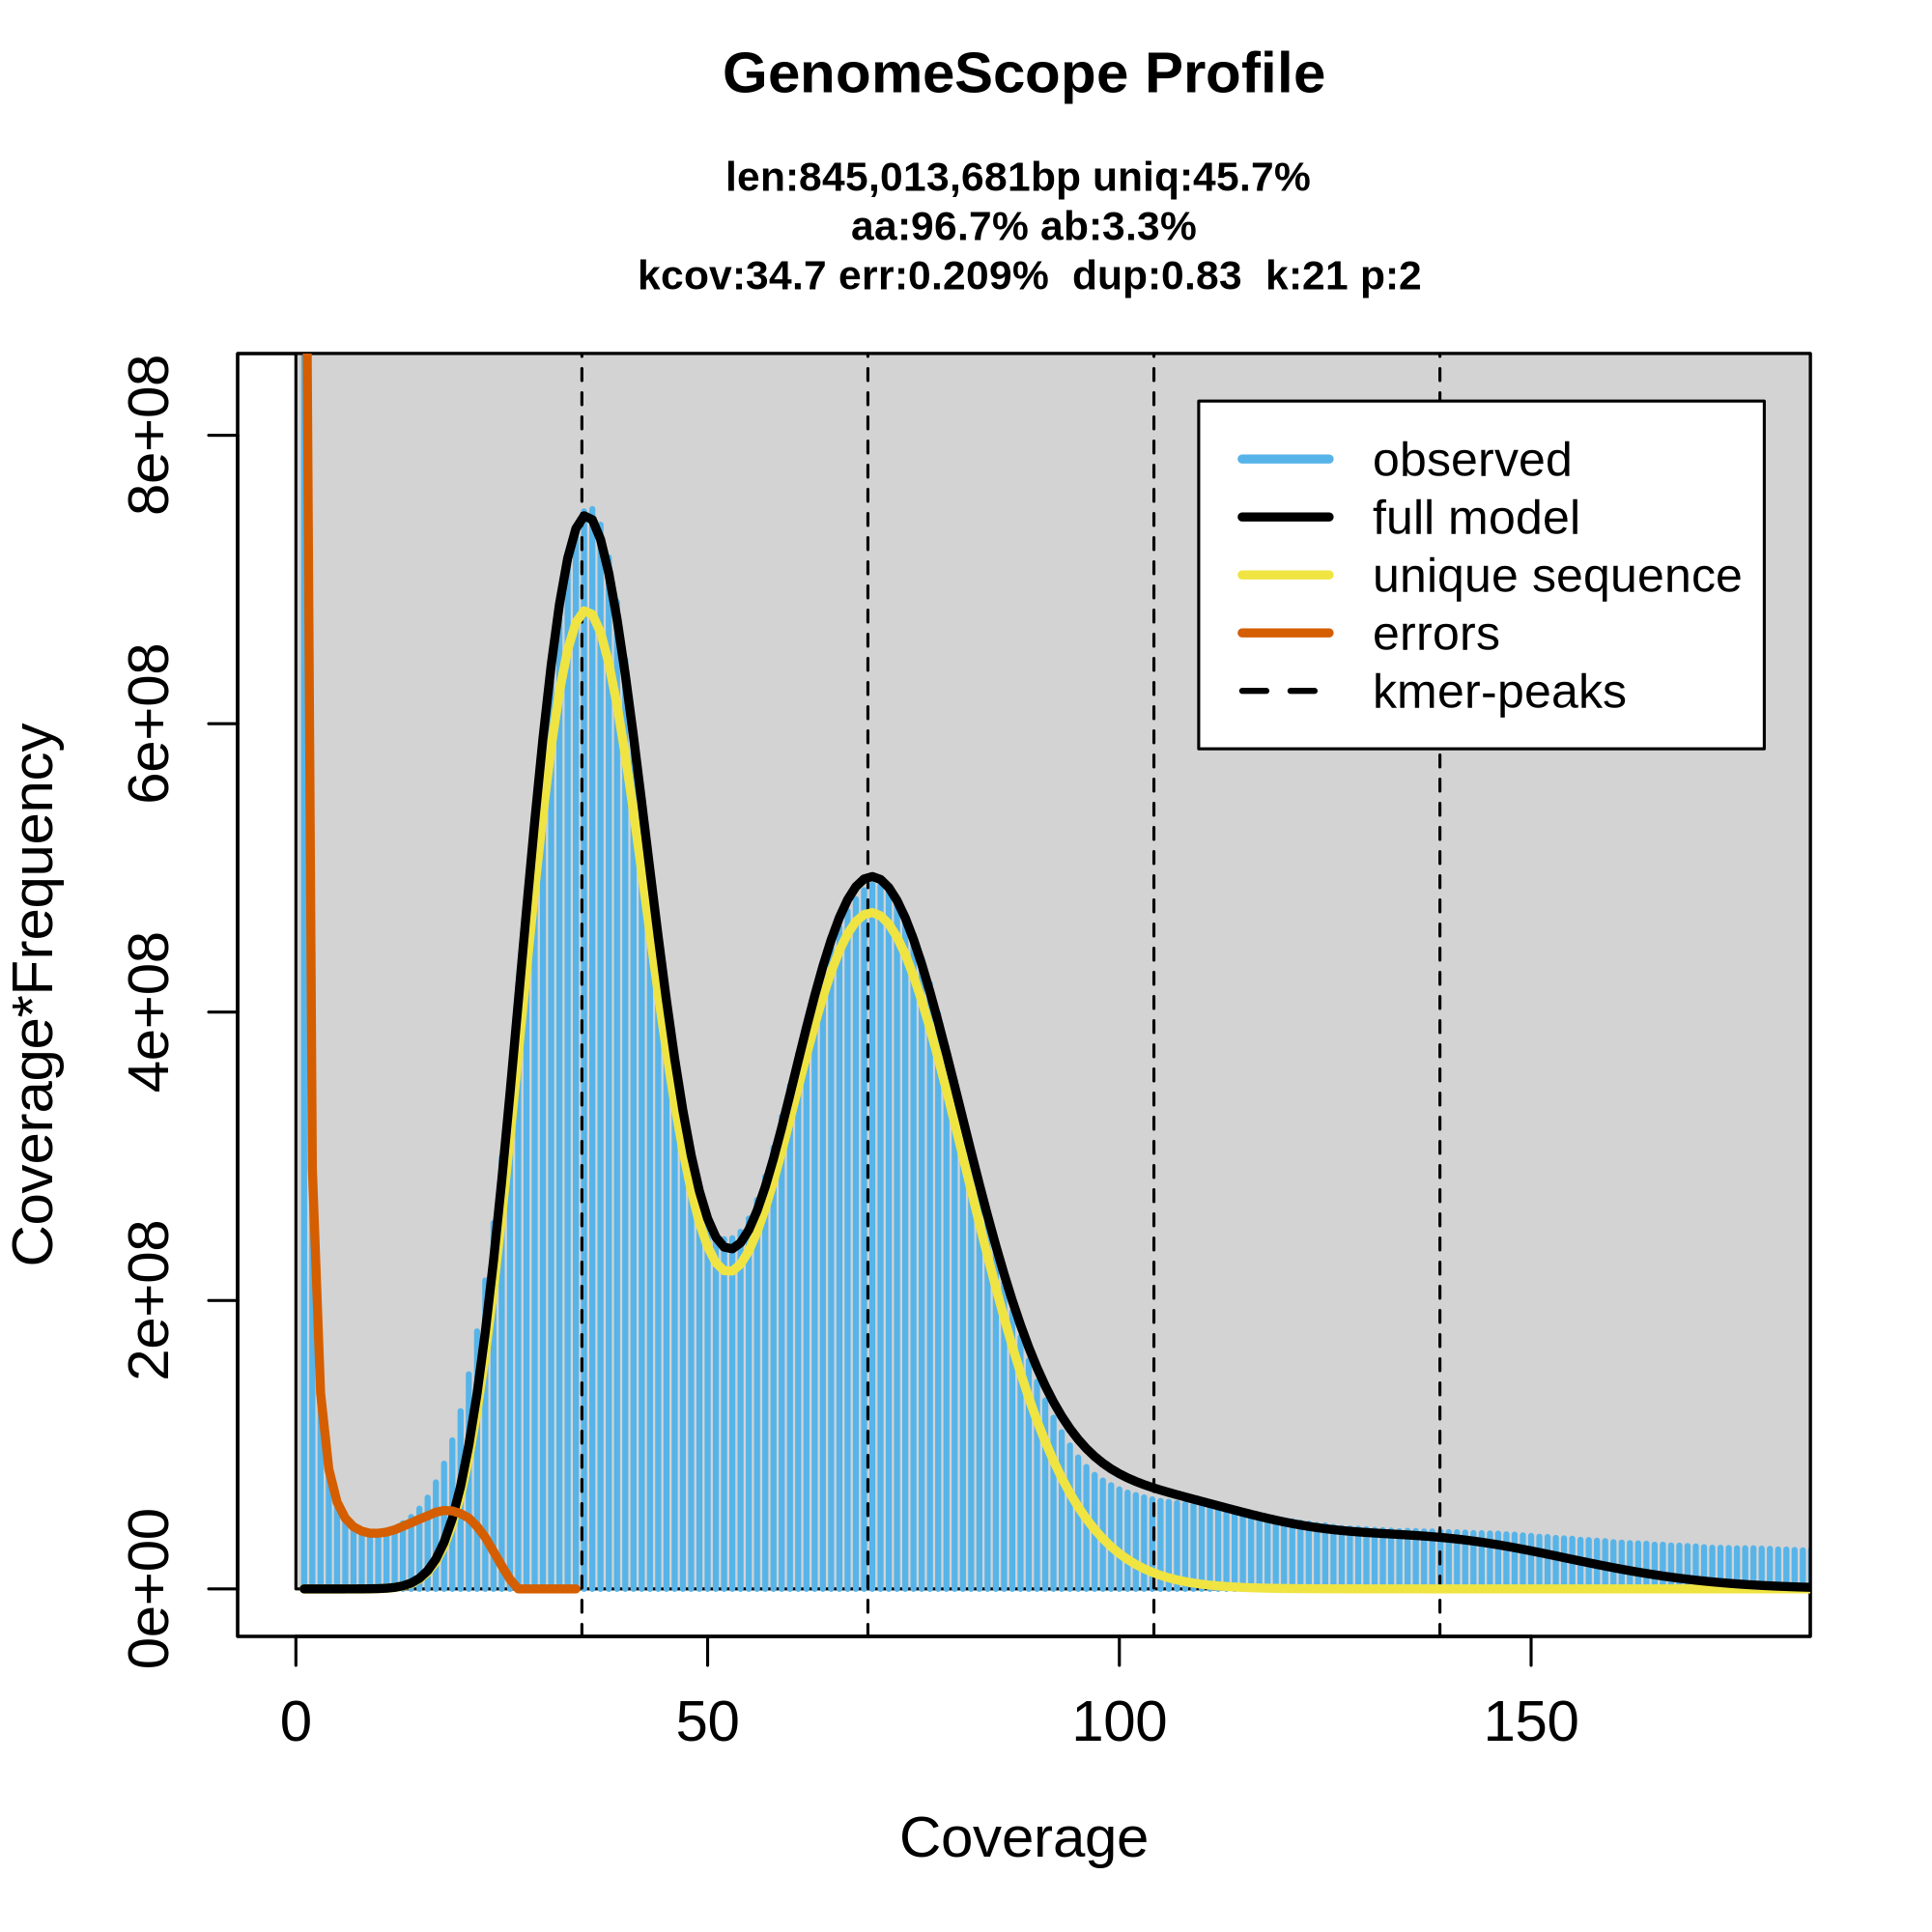
\includegraphics[width=0.8\textwidth]{figures/sups_kmers.png}
    \supfigurecaption{\textbf{\textsc{GenomeScope} profile of the raw PacBio HiFi
        data.} Distribution of 21-mers shows an estimated genome size of
        845.01 Mbp and a heterozygosity of 3.3\% in the \bgla{}
        reference assembly.}
    \label{fig:sup_kmers}
\end{figure}

% Hi-C contact map
\begin{figure}[ht]
    \centering
    \captionsetup{width=0.95\linewidth}
    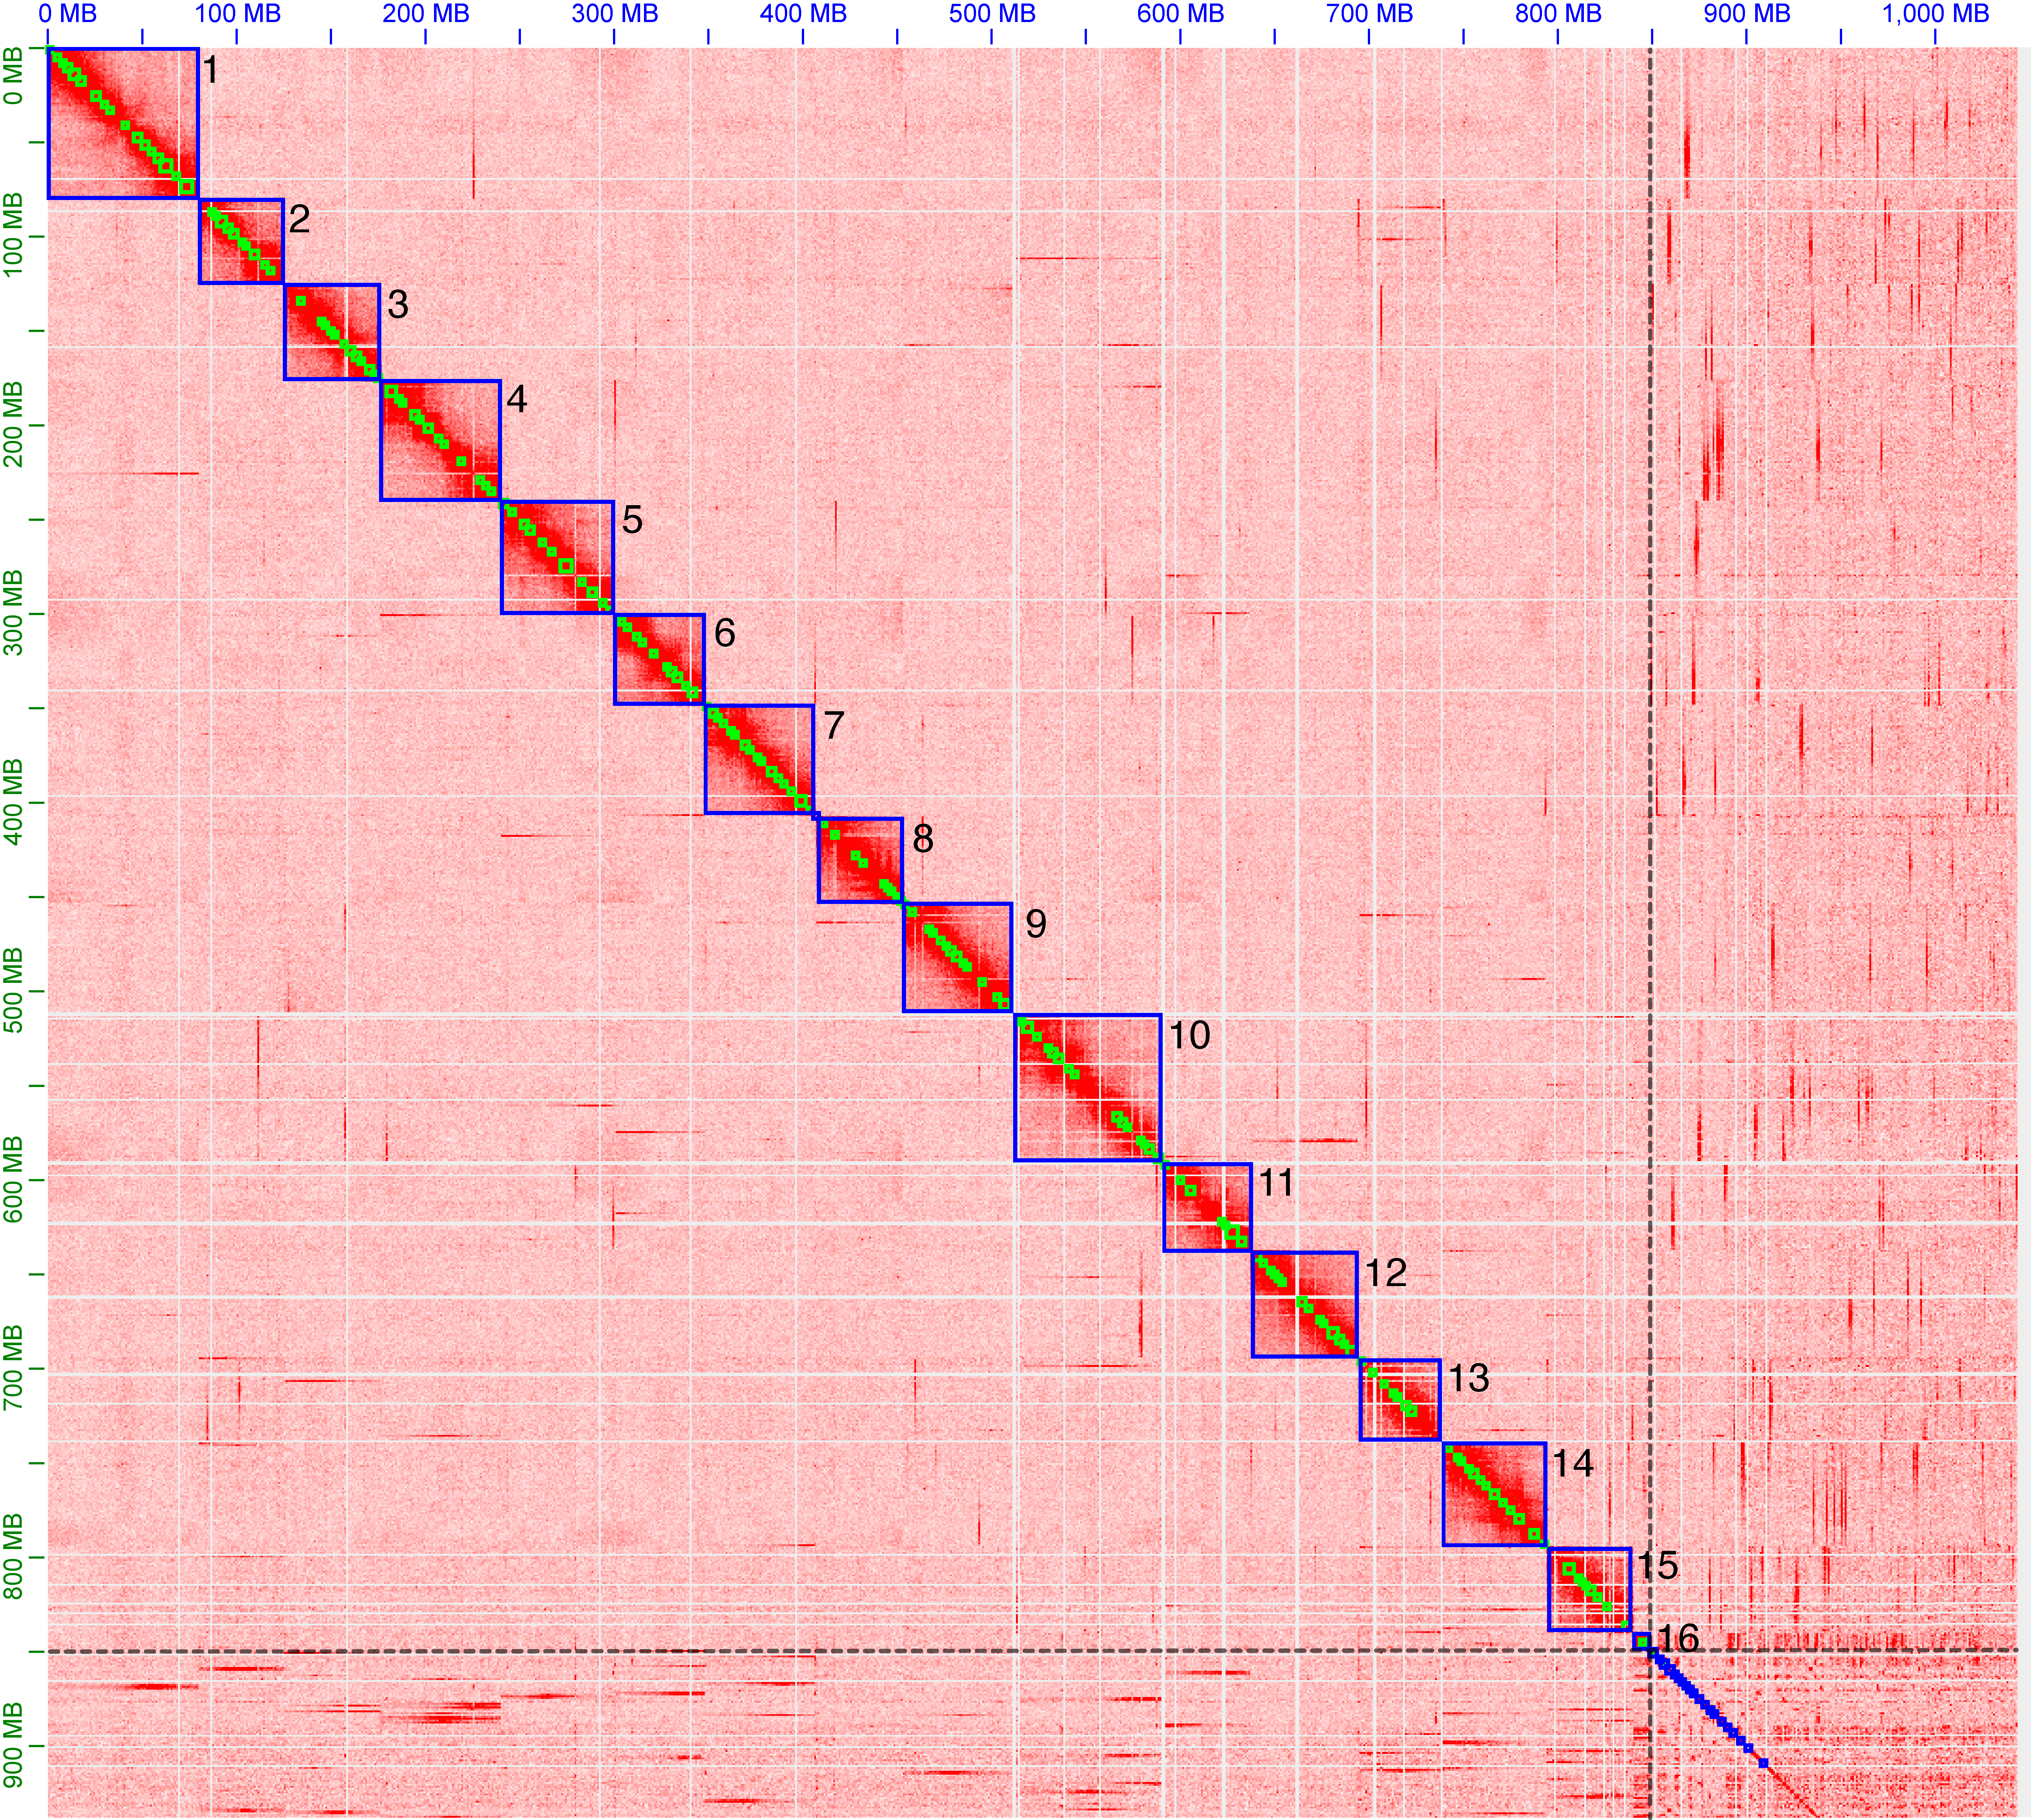
\includegraphics[width=1.0\textwidth]{figures/sups_hic.pdf}
    \supfigurecaption{\textbf{Hi-C contact map of the \balgla{} assembly.}
        The contact map shows the assembly following manual curation in
        \textsc{Juicebox}. The numbers (1--16) denote the 16 chromosome-level
        scaffolds. The dashed lines show the boundary between these 16
        chromosome-level scaffolds and the unplaced contigs. Note that this
        numbering does not reflect the final ID of the assembled sequences.
        IDs were re-assigned following additional curation and sorting of the
        sequences.}
    \label{fig:sup_hic}
\end{figure}

% dN/dS
\begin{figure}[ht]
    \centering
    \captionsetup{width=0.95\linewidth}
    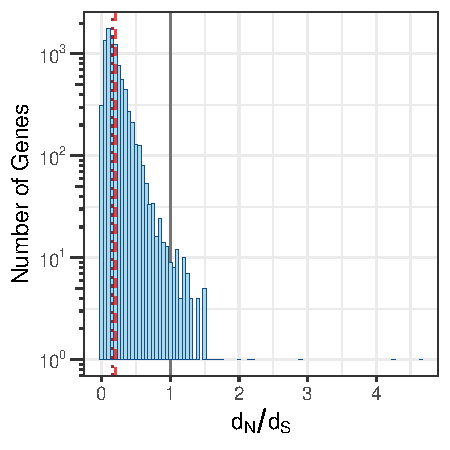
\includegraphics[width=0.7\textwidth]{figures/dnds.pdf}
    \supfigurecaption{\textbf{Distribution of the pairwise rate of non-synonymous
        to synonymous substitutions (\dnds{}).}
        The distribution is calculated across 9{,}082 single-copy orthologs
        identified between \balgla{} and \textit{Balanus
        crenatus}. The solid gray line marks the boundary between genes under
        positive selection (\dnds{} $>$ 1) and genes under purifying selection
        (\dnds{} $<$ 1). The dashed and dotted lines show the mean (0.206) and
        median (0.158) \dnds{}, both showing that on average \bgla{} coding
        sequences are evolving under a regime of purifying selection.}
    \label{fig:sup_dnds}
\end{figure}

% Direction of selection.
\begin{figure}[ht]
    \centering
    \captionsetup{width=0.95\linewidth}
    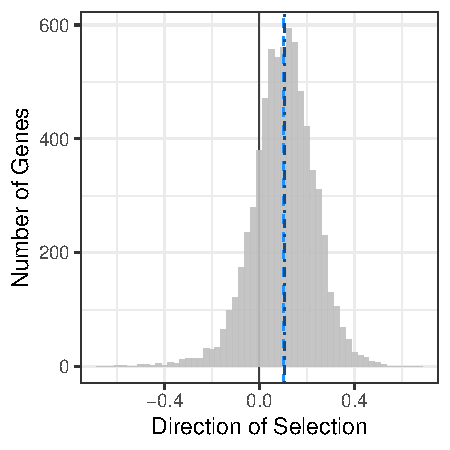
\includegraphics[width=0.7\textwidth]{figures/sups_mkt_dos.pdf}
    \supfigurecaption{\textbf{Distribution of per-gene direction of selection values.}
        The distribution shows Direction of Selection (DoS) calculated across 7{,}056
        single-copy orthologs identified between \balgla{} and
        \textit{Balanus crenatus}. The solid black line at zero marks the boundary
        between genes evolving under a regime of positive selection (DoS $>0$) and
        genes exhibiting an excess of slightly deleterious non-synonymous polymorphism
        (DoS $<0$). The light blue dashed line shows the mean DoS (0.103), while
        the dark blue dotted line shows the median DoS (0.109).
        This distribution shows that, on average, coding sequences in \bgla{} appear
        to be evolving under positive selection.}
    \label{fig:sup_dos}
\end{figure}

% Extended GO terms.
\begin{figure}[ht]
    \centering
    \captionsetup{width=0.95\linewidth}
    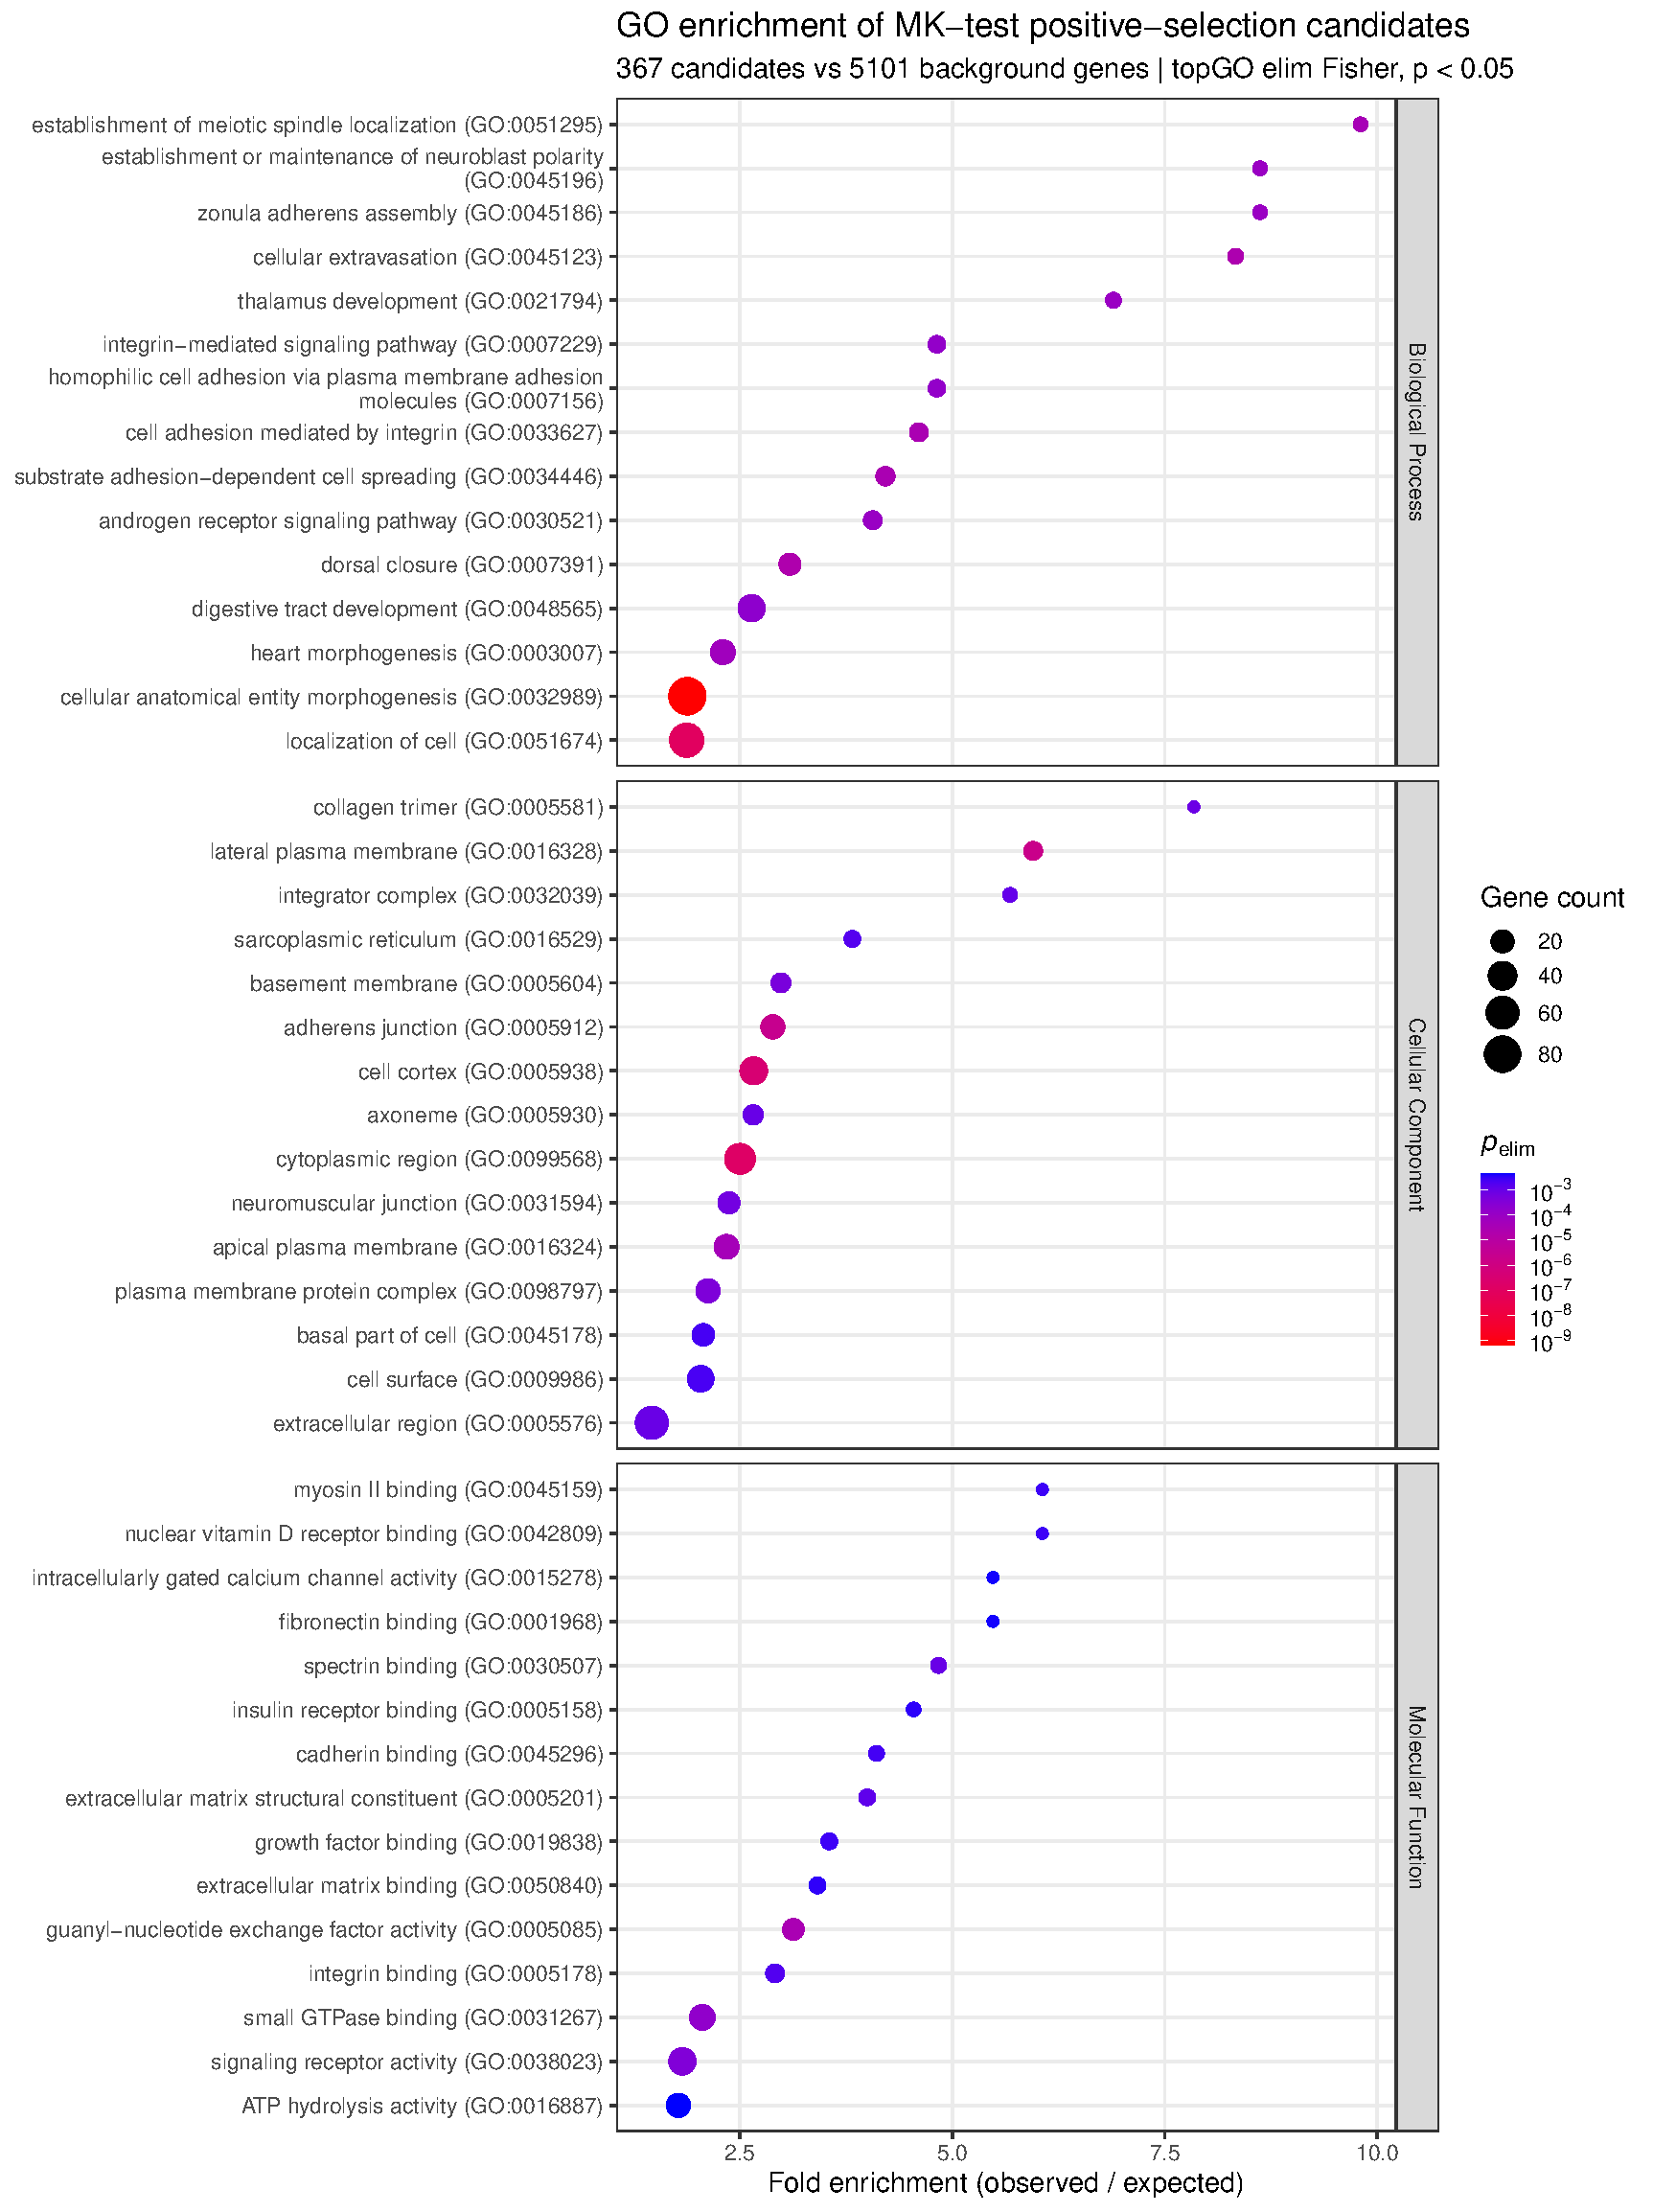
\includegraphics[width=0.925\textwidth]{figures/sups_go_extended.pdf}
    \supfigurecaption{\textbf{Significant GO term enrichment among the candidates
        under positive selection in the McDonald-Kreitman test.}
        Enrichment for the 367 candidates under selection with annotated GO terms.
        $p_\text{elim}$ denotes the $p$-value calculated from \textsc{topGO}'s
        \texttt{elim} algorithm.
        Top, middle, and bottom panels show the top 15 most enriched terms across
        the three GO categories: biological processes, cellular component, and
        molecular function.
        }
    \label{fig:sup_go}
\end{figure}

% Coding GC, GC3s, and GC4d
\begin{figure}[ht]
    \centering
    \captionsetup{width=0.95\linewidth}
    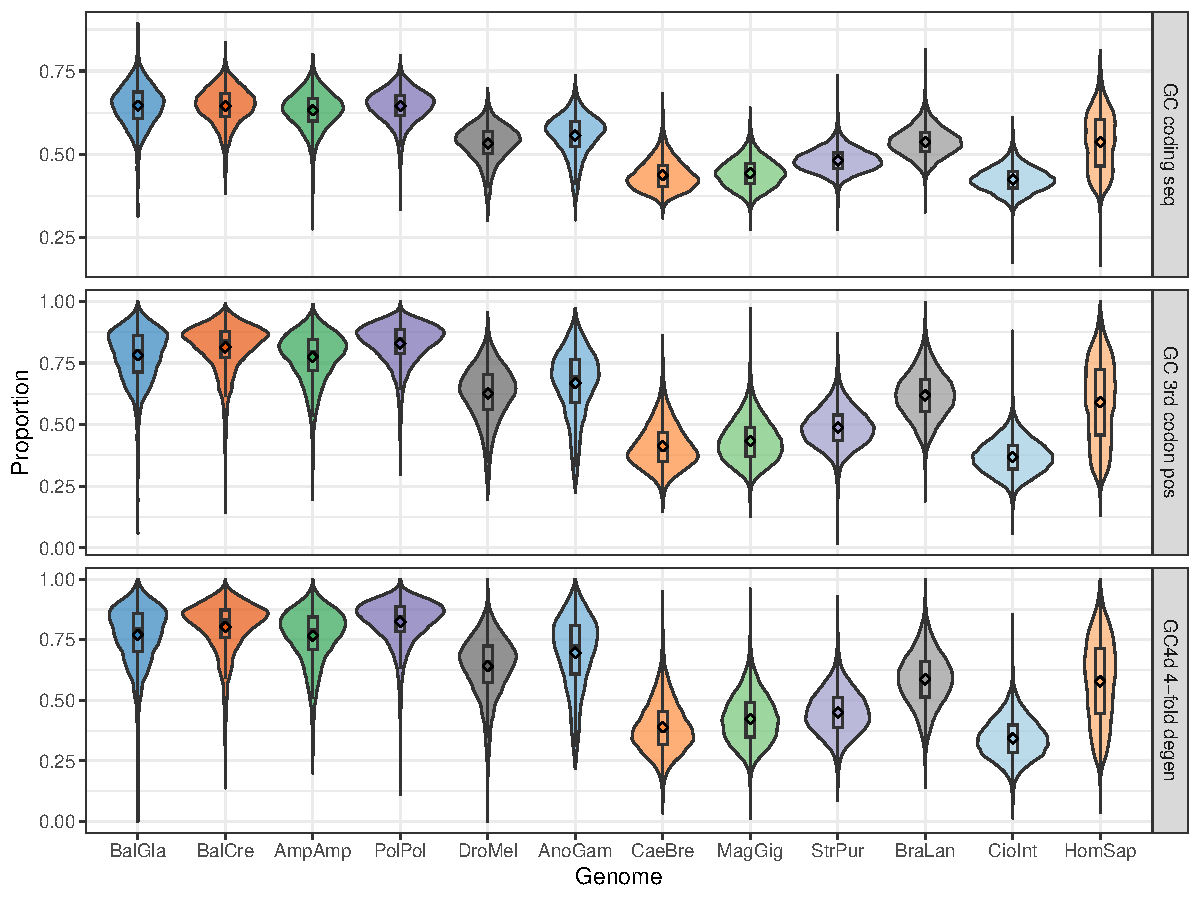
\includegraphics[width=1.0\textwidth]{figures/sups_coding_gc.pdf}
    \supfigurecaption{\textbf{Distribution of coding GC proportions across metazoan
        genomes.}
        Top, middle, and bottom panels show the GC proportions coding sequence-wide,
        at 3rd codon positions (GC3s), and at 4-fold degerate sites (GC4d),
        respectively.
        Distribution are shown across 12 metazoan genomes, including four barnacles:
        \bgla{} (\texttt{BalGla}), \textit{B. crenatus} (\texttt{BalCre}),
        \textit{A. amphitrite} (\texttt{AmpAmp}), and \textit{P. pollicipes}
        (\texttt{PolPol}).
        See Table~\ref{tab:sup_enc_summary} for additional description of the
        genomes.}
    \label{fig:sup_coding_gc}
\end{figure}

% ENC vs GC3s
\begin{figure}[ht]
    \centering
    \captionsetup{width=0.95\linewidth}
    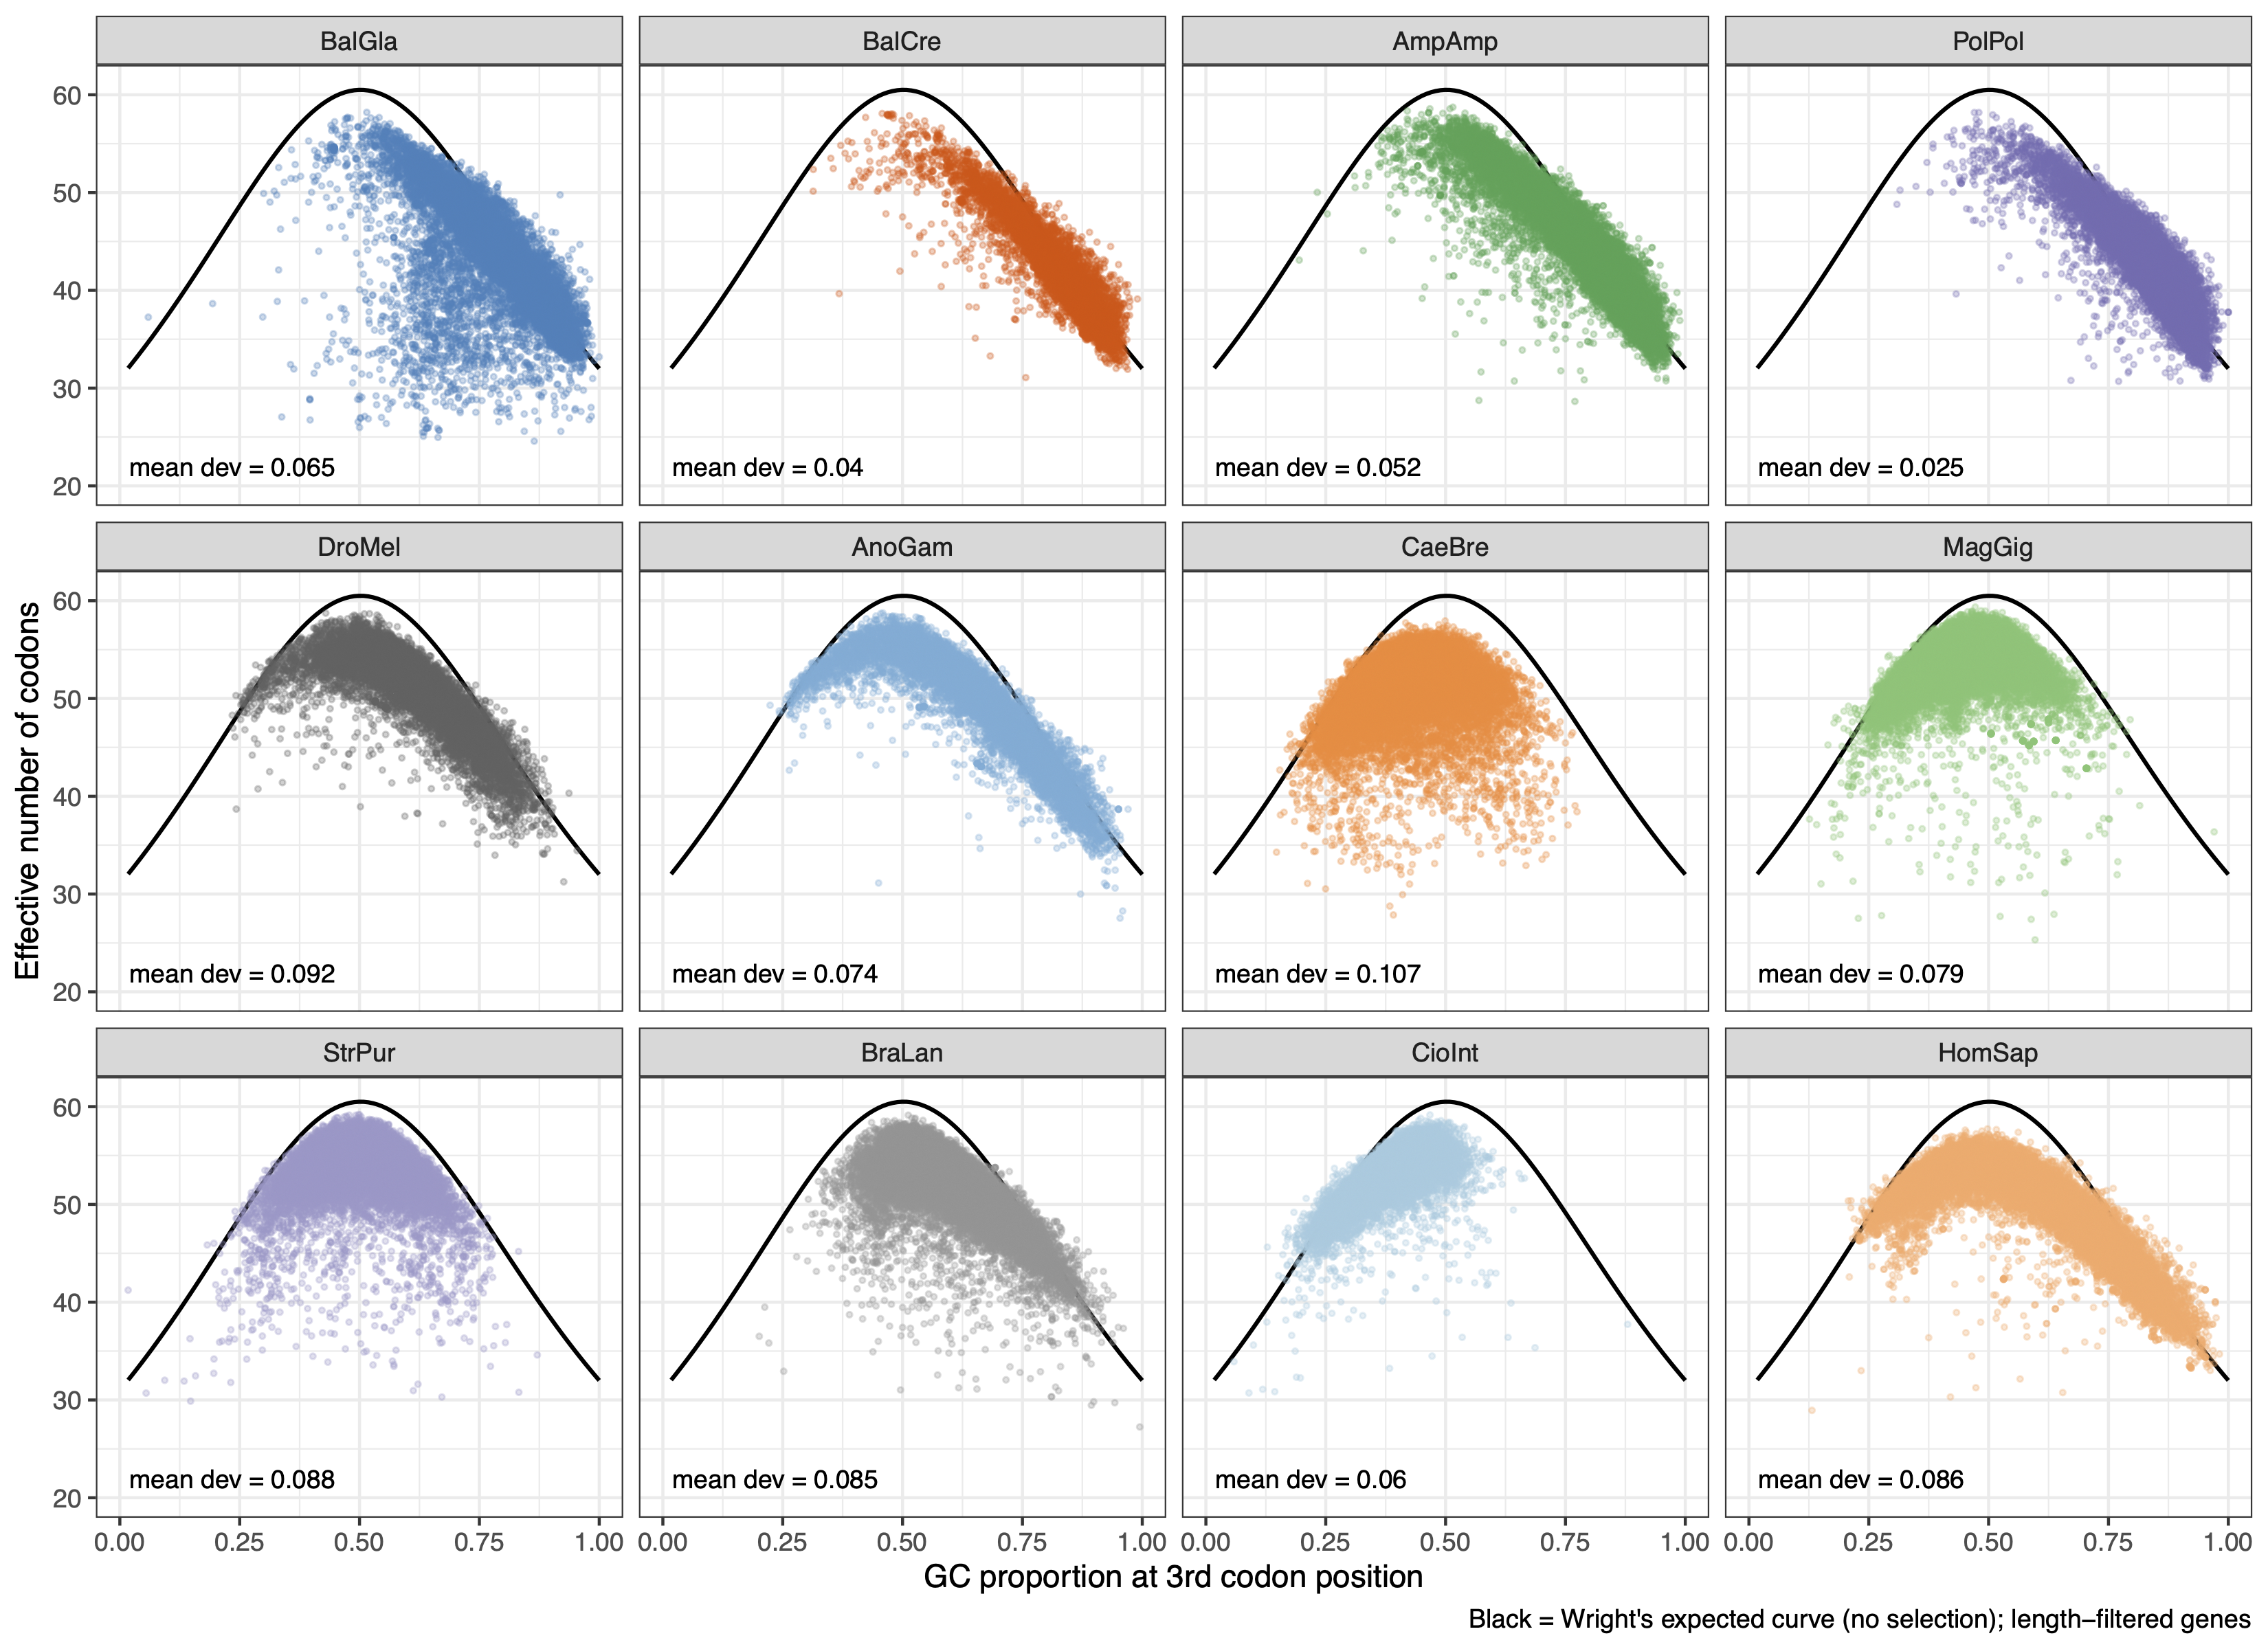
\includegraphics[width=1.0\textwidth]{figures/sups_enc_gc3s.png}
    \supfigurecaption{\textbf{Relationship between effective codons and GC content.}
        Nc-plots showing the relationship between GC proportion at 3rd codon positions
        (GC3s; X-axis) and the effective number of codons (ENC; Y-axis) for 12
        metazoan genomes.
        At each panel, each point represents a single gene.
        The black curve shows the expected relationship between GC3s and ENC, according
        to Wright's curve: \wrightenc{}, where $s$ denotes GC3s.
        The ``mean dev'' annotation shows the mean deviation in ENC from the theoretical
        expectation.
        Higher values show a larger proportion of genes showing a smaller than expected
        number of effective codons, a putative signature of translational selection.
        See Table~\ref{tab:sup_enc_summary} for additional description of the
        genomes.}
    \label{fig:sup_enc_gc3s}
\end{figure}

% Exp vs Obs ENC
\begin{figure}[ht]
    \centering
    \captionsetup{width=0.95\linewidth}
    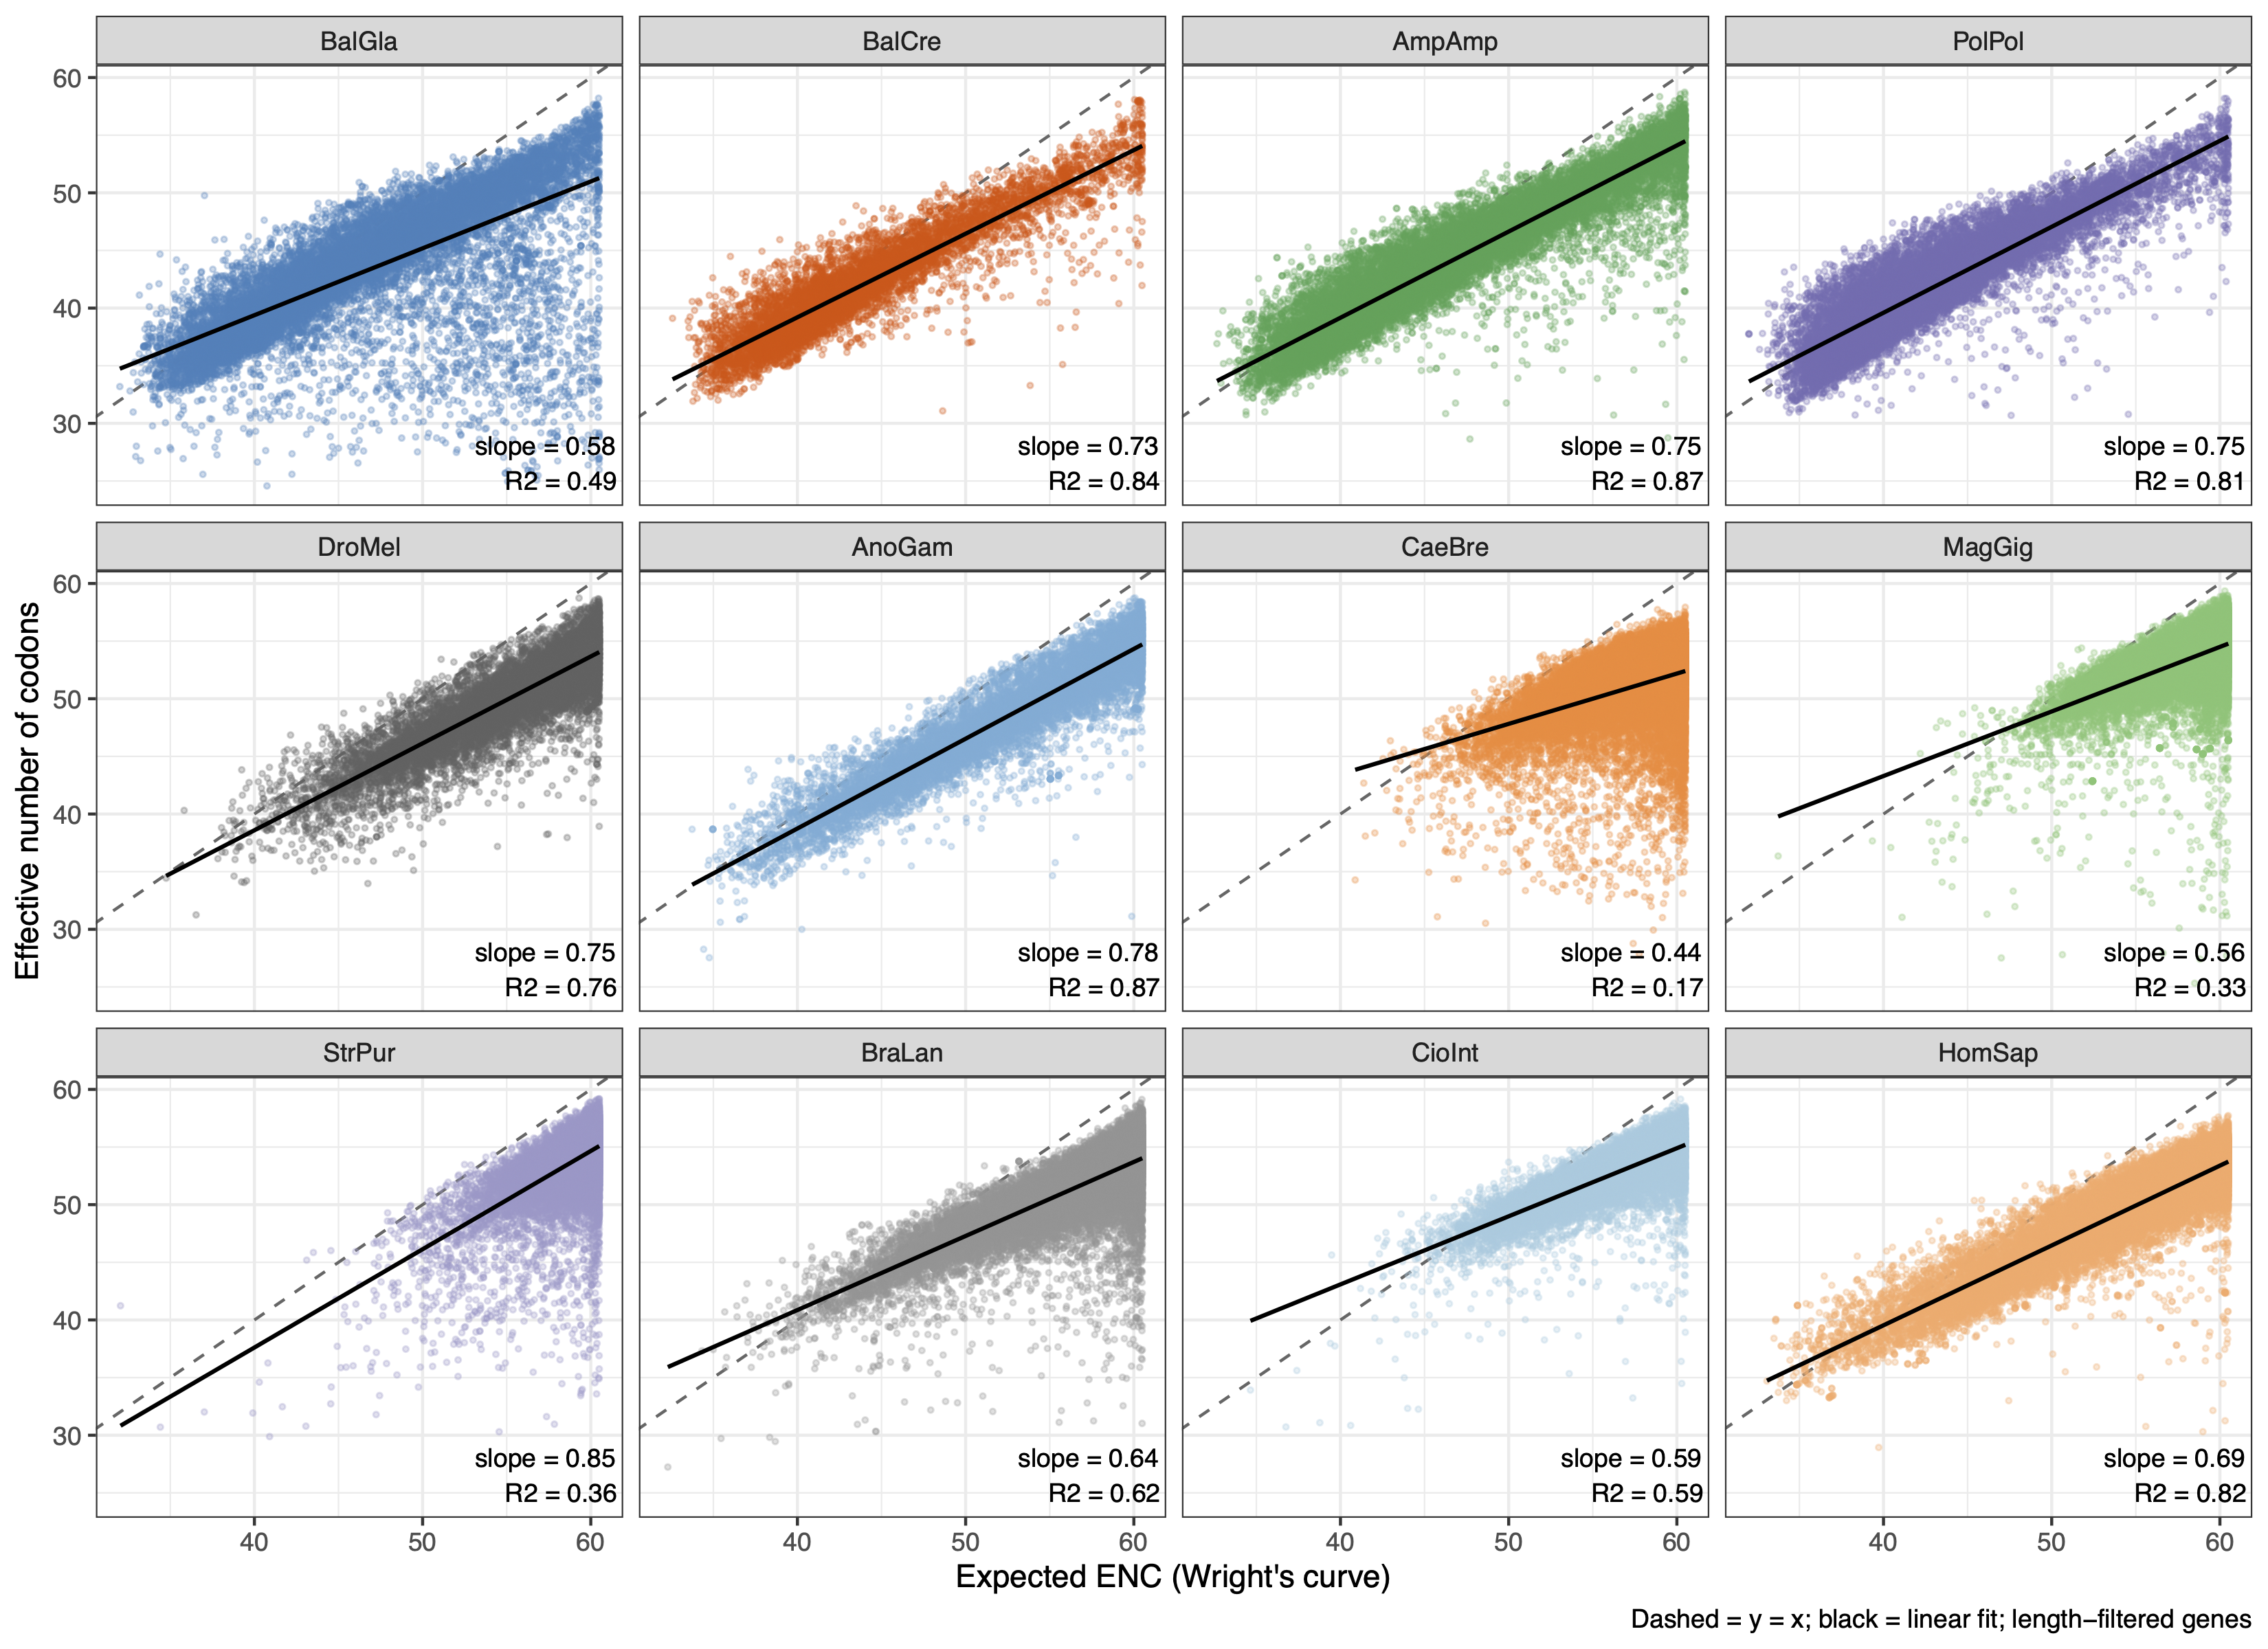
\includegraphics[width=1.0\textwidth]{figures/sups_enc_regression.png}
    \supfigurecaption{\textbf{Relationship between the expected and observed number of
        effective codons.}
        Plots show the observed effective number of codons (ENC; Y-axis) as a function
        of the expected ENC (X-axis), as defined by Wright's curve, for 12 metazoan
        genomes.
        At each panel, points represents single genes.
        Dashed line shows the one-to-one relationship, while the solid black line
        shows the linear regression.
        Annotations in the plot show the regression's slope and coefficient of
        determination ($\text{R}^2$).
        Small ($\ll1$) slopes and low $\text{R}^2$ show a reduction in the observed
        number of effective codons when compared to the theoretical expectation,
        a potential signature of translational selection.
        See Table~\ref{tab:sup_enc_summary} for additional description of the
        genomes.}
    \label{fig:sup_enc_reg}
\end{figure}

% Pi vs other species.
\begin{figure}[ht]
    \centering
    \captionsetup{width=0.95\linewidth}
    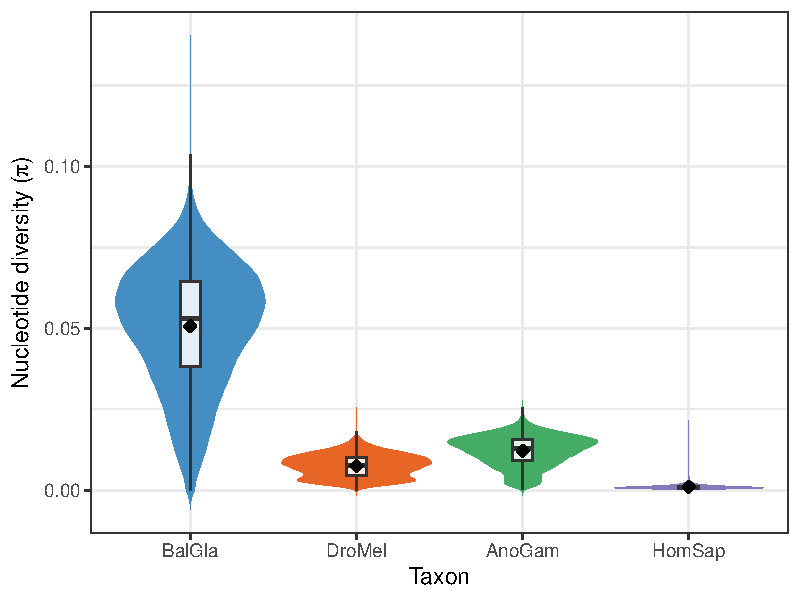
\includegraphics[width=0.9\textwidth]{figures/sups_pi_comparisons.pdf}
    \supfigurecaption{\textbf{Comparing nucleotide diversity ($\pi$) between
        barnacles and biological model systems.}
        Average $\pi$ in 10 kbp windows between the
        Oregon Pacific acorn barnacle (\balgla{}; \texttt{BalGla}),
        Sub-Saharan populations of the fruit fly (\textit{Drosophila melanogaster};
            \texttt{DroMel}),
        malaria mosquitoes from the Central African Republic (\textit{Anopheles
            gambiae}; \texttt{AnoGam}),
        and human populations of Yoruba ancestry (\textit{Homo sapiens}; \texttt{HomSap}).
        Consistent with the large \Ne{} expected for \bgla{}, this barnacle population
        exhibits an average nucleotide diversity (mean = 0.0506, median = 0.0532, standard
        deviation = 0.0188) an order of magnitude higher than \textit{Drosophila} (mean = 0.0076,
        median = 0.0078, standard deviation = 0.0035), $\approx4\times$ higher than
        \textit{An. gambiae} (mean = 0.0123, median = 0.0130, standard deviation = 0.0047), and
        $\approx48\times$ larger than diverse human cohorts (mean = 0.0011, median = $9.54\times10^{-4}$,
        standard deviation = $5.81\times10^{-4}$).}
    \label{fig:sup_pi_comp}
\end{figure}

% Pairwise correlation among different genomic feature and diversity metrics.
\begin{figure}[ht]
    \centering
    \captionsetup{width=0.95\linewidth}
    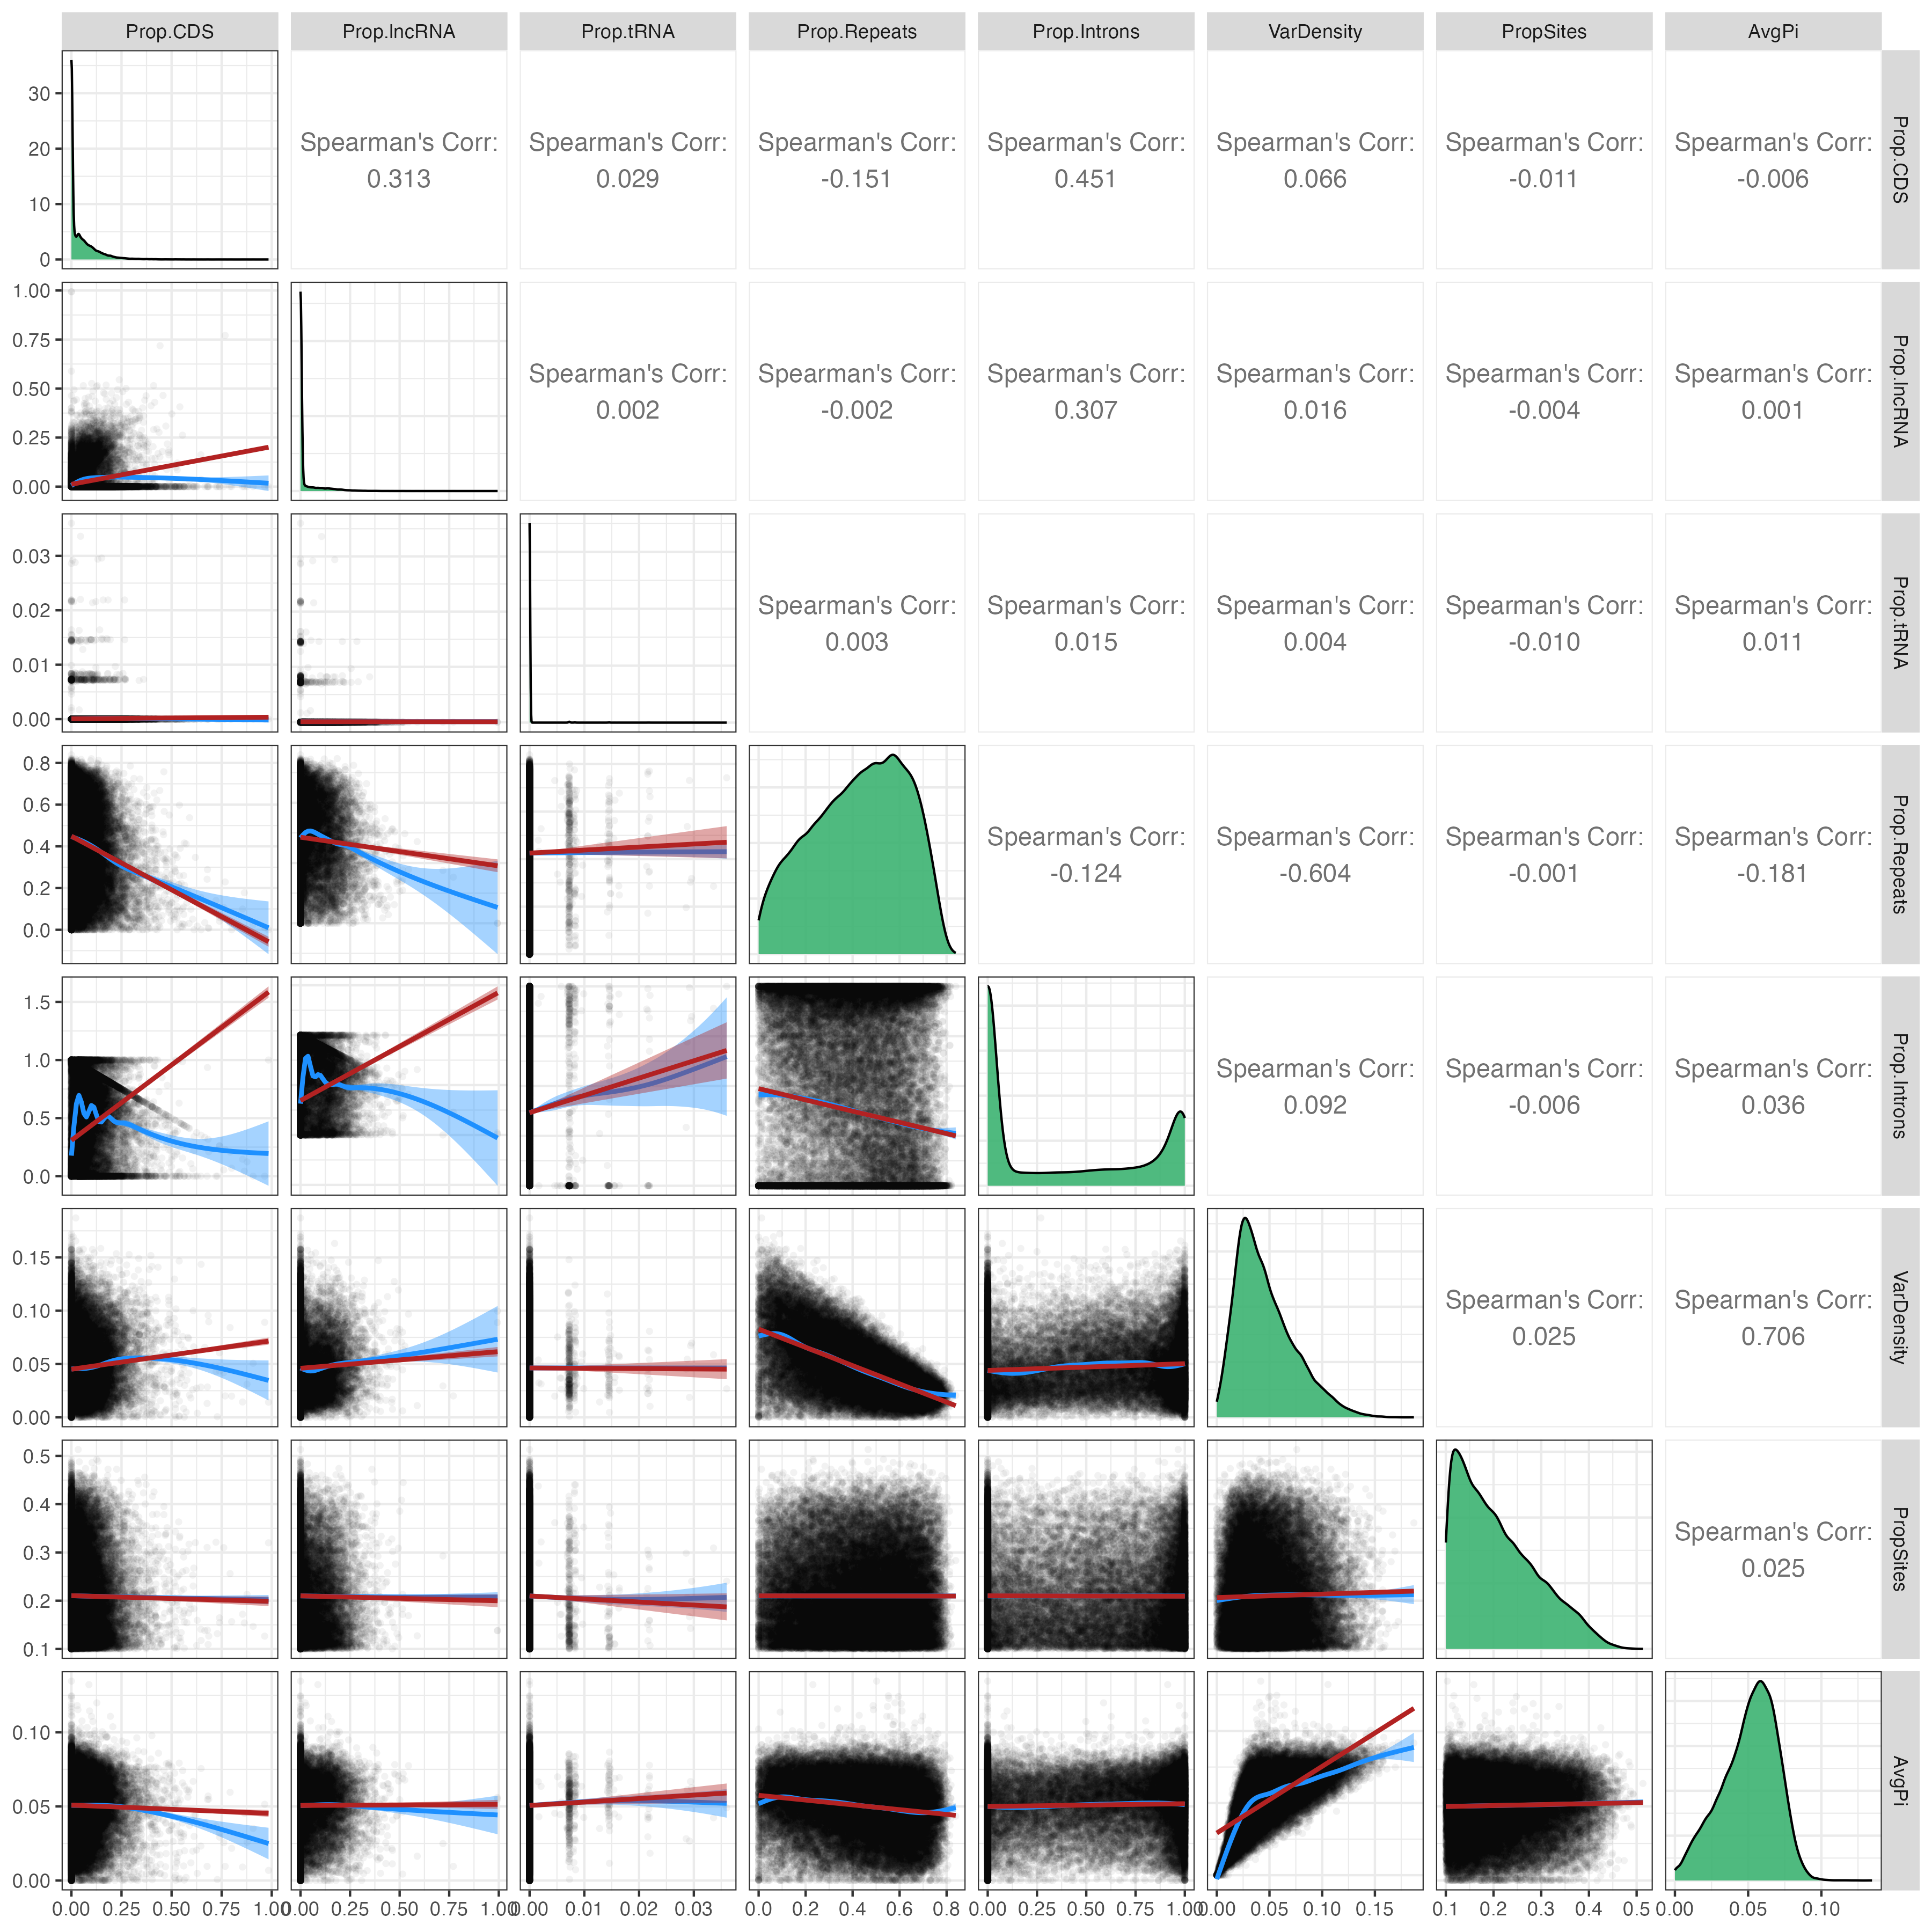
\includegraphics[width=1.0\textwidth]{figures/sups_pi_pairplot.png}
    \supfigurecaption{\textbf{Pairplot of genomic features and genetic variation
        in Oregon \balgla{}.}
        Diagonal shows the density histogram of the proportion of the genomics
        elements (e.g., CDS, lncRNA, tRNA, repeats, and introns), proportion of
        variant sites, proportion of callable sites post-filtering, and nucleotide
        diversity ($\pi$). All values computed across 10 kbp windows. Below
        the diagonal, plots show the correlation across all pairwise comparisons.
        Red and blue lines show the linear and Loess regression, respectively.
        Above the diagonal, panels show the Spearman's rank correlation
        coefficient ($\rho$) for the given pairwise comparison.}
    \label{fig:sup_pi_pairplot}
\end{figure}

% Theta_W Ne
\begin{figure}[ht]
    \centering
    \captionsetup{width=0.95\linewidth}
    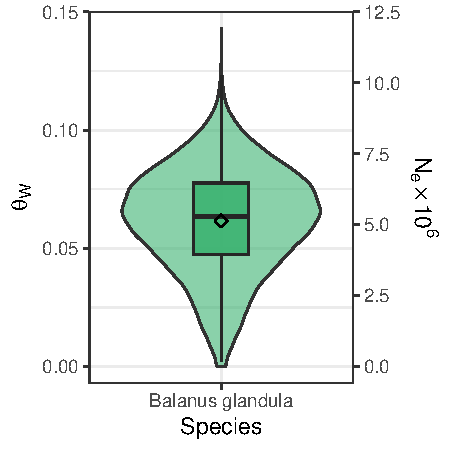
\includegraphics[width=0.7\textwidth]{figures/sups_theta_ne.pdf}
    \supfigurecaption{\textbf{Effective population (\Ne) size estimation
        of \balgla{} based on the Watterson's estimator ($\theta_\text{W}$).}
        Effective size of the population was calculated according to the
        relationship $\theta_\text{W}=4N_{e}\mu$, using a mutation rate per-base,
        per-generation ($\mu$) of $3\times10^{-9}$.
        This estimate yields a long-term \Ne{} of $\approx5.2\times10^{6}$ for
        this barnacle population.}
    \label{fig:sup_theta_ne}
\end{figure}

% msmc2 Ne
\begin{figure}[ht]
    \centering
    \captionsetup{width=0.95\linewidth}
    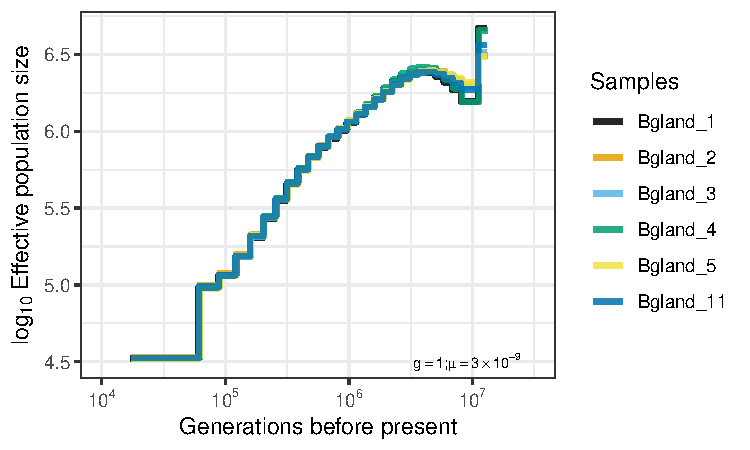
\includegraphics[width=0.9\textwidth]{figures/sups_msmc2_ne.pdf}
    \supfigurecaption{\textbf{Coalescent estimation of the effective
    population (\Ne) size estimation of \balgla{}.}
        Estimation of \Ne{} through time was done using the
        \textsc{msmc2} software, using a mutation rate per-base,
        per-generation ($\mu$) of $3\times10^{-9}$, and fixing the
        generation time ($g$) to 1.
        Each line represents the \Ne{} trajectory for each sample.
        Using just six diploid samples, and estimating only between pairs
        of unphased diploid genotypes within samples, we estimate the
        historical effective size of the population in the order of $10^{6}$
        individuals; however, we do not obtain enough resolution to resolve
        \Ne{} at recent ($<10^{5}$) time intervals.}
    \label{fig:sup_mcmc_ne}
\end{figure}



% Now this version matches the GENETICS submission.
% Start the edits from here.

% === Review Responses (extracted to a separate PDF by the Makefile) ===
% Revision build only. Records the absolute page number where the
% responses begin into review-responses-pagenum.txt so the Makefile can
% split main_revision.pdf into the manuscript and the response document.
\ifdefined\revisionmode
  \clearpage
  \newwrite\pageinfo
  \immediate\openout\pageinfo=review-responses-pagenum.txt
  \immediate\write\pageinfo{\thepage}
  \immediate\closeout\pageinfo
  \setcounter{page}{1}
  \label{review-responses-start}
  \nolinenumbers
  \pagestyle{plain}
  \fancyhead[L]{}
  \fancyhead[R]{}
  \begin{center}
  {\LARGE \textbf{Response to Reviewers}}\\[1em]
  {\large Large population sizes shape genome evolution in barnacles}
  \end{center}
  \vskip 2em
  % Cover letter and point-by-point reviewer responses.
% Reviewer text is verbatim from plosgen_review.txt; \reply{...} blocks
% are scaffolded as TODO placeholders to be filled in during the revision.
% Style adapted from the mkado-paper review-responses.tex
% (https://github.com/andrewkern/mkado-paper).
%
% This file is a body fragment: it is \input by review-responses-main.tex,
% which supplies the preamble and % Macros for reviewer responses and back-links from response document
% to manuscript line numbers. Pattern adapted from popgensbi manuscript.
%
% Expects the lineno package to be loaded by the calling document and
% \linenumbers to be active in the manuscript body.

% Reviewer / point counters
\newcommand{\thereviewer}{}
\newcounter{point}
\setcounter{point}{0}

% Start a new reviewer block. Argument is the reviewer label
% (e.g. \reviewersection{1} or \reviewersection{AE}).
\newcommand{\reviewersection}[1]{%
  \renewcommand{\thereviewer}{#1}%
  \setcounter{point}{0}%
  \section*{Reviewer \thereviewer:}%
}

% A single review point. Argument is an optional name (often empty).
% Pattern from
% http://tex.stackexchange.com/questions/2317/latex-style-or-macro-for-detailed-response-to-referee-report
\newenvironment{point}[1]
  {\color{gray}\refstepcounter{point}\bigskip\hrule\medskip\noindent
   \slshape{\fontseries{b}\selectfont (\thereviewer.\thepoint) #1}}
  {}

\newcommand{\reply}{\normalfont\medskip\noindent\textbf{Reply}:\ }

% \revpoint{R}{P} marks a manuscript line that addresses reviewer R, point P.
% Use this in the manuscript wherever you make a change in response to a
% reviewer point so the response document can back-link to it.
\newcommand{\revpoint}[2]{\hypertarget{llineno:rev#1:#2}{\linelabel{rr:rev#1:#2}}}

% \revreffull{R}{P} renders a (page, line) reference to such a target.
\newcommand{\revreffull}[2]{{(p.\ \hyperlink{llineno:rev#1:#2}{\pageref{rr:rev#1:#2}, l.\ \lineref{rr:rev#1:#2}})}}

% \revref expands to the page/line reference for the current reviewer/point
% inside a {point} environment.
\newcommand{\revref}{\revreffull{\thereviewer}{\thepoint}\xspace}

% Named back-links: place \llabel{name} in the manuscript, refer to it
% from anywhere with \llname{name}.
\newcommand{\llabel}[1]{\hypertarget{ll:#1}{\linelabel{#1}}}
\newcommand{\llname}[1]{{(p.\ \hyperlink{ll:#1}{\pageref{#1}, l.\ \lineref{#1}})}}

% Italics-quoted block (used to set off the verbatim reviewer text).
\newenvironment{itquote}
  {\begin{quote}\color{gray}\itshape}
  {\end{quote}}

% Convenience macros
\newcommand{\rollover}{\reply{The reviewer makes an excellent point that we have missed out entirely. We have made all the changes suggested, down to the minutiae \revref.}}
\newcommand{\playdead}{\reply{The reviewer makes an excellent point. We have made an utterly trivial change \revref{}that we think deals entirely with the concern raised.}}

% lineno + amsmath fix: lineno doesn't number lines inside align/equation
% environments by default. Patch from
% http://tex.stackexchange.com/questions/43648
\ifcsname patchAmsMathEnvironmentForLineno\endcsname
\else
\newcommand*\patchAmsMathEnvironmentForLineno[1]{%
  \expandafter\let\csname old#1\expandafter\endcsname\csname #1\endcsname
  \expandafter\let\csname oldend#1\expandafter\endcsname\csname end#1\endcsname
  \renewenvironment{#1}%
    {\linenomath\csname old#1\endcsname}%
    {\csname oldend#1\endcsname\endlinenomath}}
\newcommand*\patchBothAmsMathEnvironmentsForLineno[1]{%
  \patchAmsMathEnvironmentForLineno{#1}%
  \patchAmsMathEnvironmentForLineno{#1*}}
\AtBeginDocument{%
  \patchBothAmsMathEnvironmentsForLineno{equation}%
  \patchBothAmsMathEnvironmentsForLineno{align}%
  \patchBothAmsMathEnvironmentsForLineno{flalign}%
  \patchBothAmsMathEnvironmentsForLineno{alignat}%
  \patchBothAmsMathEnvironmentsForLineno{gather}%
  \patchBothAmsMathEnvironmentsForLineno{multline}%
}
\fi
.

\begin{minipage}[b]{2.6in}
  Resubmission Cover Letter \\
  {\it PLOS Genetics} \\
  Manuscript PGENETICS-D-26-00481
\end{minipage}
\hfill
\begin{minipage}[b]{3.4in}
  Angel G.\ Rivera-Col\'on (on behalf of all authors) \\
  \today
\end{minipage}

\vskip 2em

\noindent
{\bf Dear Dr.\ Bergland,}

\vskip 1em

TODO

\vskip 2em

\noindent\hspace{4em}
\begin{minipage}{4.5in}
\noindent
{\bf Sincerely,}

\vskip 2em

{\bf
  Angel G.\ Rivera-Col\'on (on behalf of all authors)
}\\
\end{minipage}

\vskip 4em

\pagebreak

%%%%%%%%%%%%%%%%%%%%%%%%%%%%%%%%%%%%%%%%%%%%%%%%%%%%%%%%%%%%%%%%%%%%%%%%%
\reviewersection{AE}

\begin{itquote}
This manuscript has been reviewed by three expert reviewers as well as
myself. We appreciated the thoroughness of the analysis, and generally
found the writing clear. There was also a shared sentiment that (1) the
focus on genome assembly of hyperpolymorphic species was put forward as
a central aspect of the paper, but there was no assessment presented
that this was the ``best way to do the assembly''; (2) the section on
allozymes fell short because of the limited sampling of individuals (and
no mention of intentional sampling across tidal height suggests that the
relevant haplotypes may have not been sampled); (3) there are multiple
places where the presentation of results could be improved; and (4)
there was insufficient or inaccurate representations of the published
literature. I agree with all of the reviewer's comments. Although the
paper is strong technically, the conceptual advances presented by the
authors are not strong enough for PLOS Genetics. We encourage
resubmission to PLOS Genetics if the authors can incorporate additional
spatial sampling/sequencing across broad (latitudinal) or local
(intertidal height) scales.
\end{itquote}

\reply{%
  \textsc{TODO} --- overall response to the editor.
}

%---------- AE.1 ----------
\begin{point}{} % AE.1 -- Nunez et al. 2021 mischaracterized
Lines 95--98, the authors cite Nunez et al.\ 2021 as an example of a
study focusing on \emph{Mpi}, and follow with a statement that ``this
work has been restricted to a handful of loci\ldots'' That is not a
fair reading of Nunez 2021, which conducted whole-genome pooled
resequencing. To be fair, the reference genome they used was not perfect
but I think that Nunez 2021 does more than you give it credit for.
\end{point}

\reply{%
  \textsc{TODO} --- author response (cite the manuscript change with \texttt{\textbackslash revref}).
}

%---------- AE.2 ----------
\begin{point}{} % AE.2 -- speculative gene function in Results
Lines 228--236. Although the function of these genes may not be
speculative, the discussion of their function as it relates to positive
selection is highly speculative and does not seem relevant for the
Results section.
\end{point}

\reply{%
  \textsc{TODO} --- author response.
}

%---------- AE.3 ----------
\begin{point}{} % AE.3 -- topic sentence at line 271 / trim function speculation
Line 271. This sentence is not a good topic sentence for the paragraph
as it jumps right into the tubular gene and discusses it as the single
example of excess polymorphism. After discussing this gene, the rest of
the paragraph is about genes showing evidence of positive selection. I
suggest that you retool the topic sentence. Also, to reiterate my
comment above --- the function of these genes is not a result of your
work. It is a speculative interpretation about how the likely function
of these genes is the target of flavors of selection. It is probably not
necessary and could be trimmed to make the paper a bit shorter.
\end{point}

\reply{%
  \textsc{TODO} --- author response.
}

%---------- AE.4 ----------
\begin{point}{} % AE.4 -- p-value correction method (Fig 3 legend, throughout)
Figure 3 legend (and throughout). What method did you use to correct
p-values?
\end{point}

\reply{%
  \textsc{TODO} --- author response.
}

%---------- AE.5 ----------
\begin{point}{} % AE.5 -- parenthetical citation style / PLOS numbering
Parenthetical citations: Please correct the style of the parenthetical
citations (and possibly bibliography) to conform to PLOS G's style.
Citations are neither in alphabetical order nor chronological order;
more than one author are listed for pubs with more than two authors;
sometimes there are initials for first \& middle names, sometimes not. I
think PLOS G has numerically ordered citations.
\end{point}

\reply{%
  \textsc{TODO} --- author response.
}

%---------- AE.6 ----------
\begin{point}{} % AE.6 -- intertidal stratification of Mpi sampling
Line 295--351. The classic story from \emph{Semibalanus} is that
\emph{Mpi} is stratified based on position in the intertidal. You all
collected six barnacles but did not, apparently, specifically stratify
on intertidal height. Therefore, you could have missed an important
allelic class (either due to sampling a single position in the
intertidal, or just chance).
\end{point}

\reply{%
  \textsc{TODO} --- author response.
}

%---------- AE.7 ----------
\begin{point}{} % AE.7 -- Figure 4 / Fig S7 tiny text
Figure 4. The text in this figure is tiny. Consider improving for
readability. Same goes for Fig.\ S7.
\end{point}

\reply{%
  \textsc{TODO} --- author response.
}

%---------- AE.8 ----------
\begin{point}{} % AE.8 -- repeats vs diversity claim (lines 376-379)
Lines 376--379. It is a little hard to assess the veracity of this
claim. For example, there is a correlation coefficient of $-0.181$
between $\pi$ and the proportion of repeats (Fig.\ S11). Is that
coefficient statistically different from zero? I bet it is. And, those
conspicuous dips in $\theta_\pi$ and Watterson's $\theta$ at the center
of each chromosome sure do look like centromeres. Do barnacles have
metacentric chromosomes? Also, what are you calling ``repeats'' in 6B?
Could that be anything from a microsat to a TE? How does this
correlation change if you focus only on TEs?
\end{point}

\reply{%
  \textsc{TODO} --- author response.
}

%---------- AE.9 ----------
\begin{point}{} % AE.9 -- "see below" dangling reference
Line 379: ``see below''. See below where?
\end{point}

\reply{%
  \textsc{TODO} --- author response.
}

%---------- AE.10 ----------
\begin{point}{} % AE.10 -- assembly-methods discussion section length
Lines 424--462. I found this section challenging as the first section of
the discussion. You don't really evaluate different methods / approaches
for genome assembly in a highly heterozygous species. Consider reducing
length.
\end{point}

\reply{%
  \textsc{TODO} --- author response.
}

\pagebreak

%%%%%%%%%%%%%%%%%%%%%%%%%%%%%%%%%%%%%%%%%%%%%%%%%%%%%%%%%%%%%%%%%%%%%%%%%
\reviewersection{1}

\begin{itquote}
The authors generated a chromosome-level genome assembly for
\emph{Balanus glandula}, an ecologically important and well-studied
barnacle species in West Coast rocky shore ecosystems. This genome
assembly is of high quality and will be a useful resource for future
evolutionary studies on this species. Additionally, analyses of this
genome assembly, a draft assembly of a congener, and WGS data of 6
individuals from one population, provide insights into the evolutionary
dynamics of species with large population sizes and highly heterozygous
genomes. Overall, the manuscript is well-written, and the methodology is
thorough. However, I have a handful of comments about the manuscript,
which will help ground these analyses in greater taxonomic and
ecological context.
\end{itquote}

\reply{%
  \textsc{TODO} --- overall response to Reviewer~1.
}

%---------- R1.1 ----------
\begin{point}{} % 1.1 -- life history details in the Introduction
In the Introduction there should be increased information about the life
history of the species since these details are pertinent for
understanding demographic and selection processes in the species. For
example, how long is the planktonic larval duration? What is their mode
of reproduction? What is the timing of spawning? How many offspring are
produced per individual?
\end{point}

\reply{%
  \textsc{TODO} --- author response.
}

%---------- R1.2 ----------
\begin{point}{} % 1.2 -- spatial/temporal variation, linear coastline, dispersal
This manuscript focuses extensively on the fact that \emph{B.\ glandula}
is a species with large population sizes. However, there is a large
amount of spatial and temporal variation in \emph{B.\ glandula}
reproductive output, recruitment, and abundance along the west coast,
across both small and large scales (e.g., Gaines, Brown \& Roughgarden
1985; Berger 2009; Broitman et al.\ 2008; MARINe long-term monitoring
data). Additionally, the coastline is linear in nature creating unique
patterns of dispersal and gene flow. These dynamics greatly impact how
evolutionary processes function in this species --- e.g., there is a low
likelihood of adaptation to local conditions since planktonic larvae
from one population often disperses to another population. These dynamics
need to be noted in the Introduction and there should be greater
interpretation of what the genomic patterns of high heterozygosity,
strong positive selection, etc.\ mean within the context of the life
history and ecology of this particular species.
\end{point}

\reply{%
  \textsc{TODO} --- author response.
}

%---------- R1.3 ----------
\begin{point}{} % 1.3 -- novelty of assembly methodology in Results
Given that some of the motivation in the Introduction focuses on the
difficulty in assembling genomes for species with high heterozygosity,
more information should be provided in the results of the genome assembly
to indicate the novelty of the methodology used to produce a very
complete assembly with low duplicates.
\end{point}

\reply{%
  \textsc{TODO} --- author response.
}

%---------- R1.4 ----------
\begin{point}{} % 1.4 -- microhabitat variation and sampling design
More information is needed about the sampling of the individuals from
the Oregon population. It is stated in the Discussion that ``intertidal
microhabitat is approximately uniform in our central Oregon sampling''.
The central Oregon rocky coastline, including Cape Perpetua where the
samples were collected for the WGS, is a dynamic environment with high
levels microhabitat variation (e.g., Sanford \& Menge 2001 provides
evidence that variation in wave exposure within a site influences
post-settlement mortality of barnacle and growth rate). Also, given that
previous research on barnacles has shown that variation in allozyme loci
are associated with spatial heterogeneity (Hedgecock 1994, Schmidt \&
Rand 1999; Nunez et al.\ 2020), why was microhabitat not considered prior
to sampling, as lack of this information greatly weakens the
interpretability of patterns from the data.
\end{point}

\reply{%
  \textsc{TODO} --- author response.
}

%---------- R1.5 ----------
\begin{point}{} % 1.5 -- main-text table of genome statistics
Since a large focus of this manuscript is the generation of the genome
assembly for \emph{B.\ glandula}, the manuscript would benefit from a
table in the main text that summarizes the key genome statistics of the
final assembly --- total length, N50, BUSCO completeness values, etc.\
--- values that are currently in Table S1.
\end{point}

\reply{%
  \textsc{TODO} --- author response.
}

%---------- R1.6 ----------
\begin{point}{} % 1.6 -- B. glandula in middle row of synteny plot (Fig 1)
Since the focus of the manuscript is on \emph{B.\ glandula}, for the
synteny plot in Figure 1, \emph{B.\ glandula} should be in the middle
row, since it would be easier to see the associations of \emph{B.\
glandula} with the other two barnacle species.
\end{point}

\reply{%
  \textsc{TODO} --- author response.
}

%---------- R1.7 ----------
\begin{point}{} % 1.7 -- gene names on Figure 3
To improve the utility of figure 3 in conveying information, it could be
useful to state the gene names on Figure 3 that are mentioned in the
text.
\end{point}

\reply{%
  \textsc{TODO} --- author response.
}

%---------- R1.8 ----------
\begin{point}{} % 1.8 -- Figure 4 axes and legend legibility
The axes and legend for Figure 4 should be bigger to make it easier to
read.
\end{point}

\reply{%
  \textsc{TODO} --- author response.
}

%---------- R1.9 ----------
\begin{point}{} % 1.9 -- congeners terminology and Gpi species attribution
Congeneric barnacles are barnacles belonging to the same genus. Thus,
\emph{Semibalanus balanoides} and \emph{Balanus glandula} are not congers
(line 582). Also, the patterns of variation in \emph{Gpi} identified in
Flight \& Rand 2012 and stated in the following sentence were identified
in \emph{S.\ balanoides}. Thus, it would be more appropriate to state the
species name rather than mention `other marine invertebrates', as that
insinuates that patterns in \emph{Gpi} have been identified more broadly
across marine invertebrate taxa.
\end{point}

\reply{%
  \textsc{TODO} --- author response.
}

%---------- R1.10 ----------
\begin{point}{} % 1.10 -- "small propagule size" (line 612)
It is stated in the Discussion that \emph{B.\ glandula} has ``small
propagule size'' (line 612). \emph{B.\ glandula} is a simultaneous
hermaphrodite that broods its offspring, and releases about 30,000 larvae
per brood (Newman \& Abbott 1980). Thus, similar to many other marine
invertebrates that broadcast spawn, the species has high fecundity and
high levels of early life mortality.
\end{point}

\reply{%
  \textsc{TODO} --- author response.
}

%---------- R1.11 ----------
\begin{point}{} % 1.11 -- methods thorough (positive)
The methods are incredibly thorough and easy to follow.
\end{point}

\reply{%
  \textsc{TODO} --- author response.
}

%---------- R1.12 ----------
\begin{point}{} % 1.12 -- broken code link, data preview for reviewers
The link for the code is not working. Also, the final assembly and
annotation files should be available for preview to reviewers.
\end{point}

\reply{%
  \textsc{TODO} --- author response.
}

%---------- R1.13 ----------
\begin{point}{} % 1.13 -- Line 205: repeated word "consistent"
Line 205: For clarity in reading, change one of the words ``consistent''
to something else, since it is used twice within the same sentence.
\end{point}

\reply{%
  \textsc{TODO} --- author response.
}

%---------- R1.14 ----------
\begin{point}{} % 1.14 -- Line 234: citation initials error (Cheng et al. 2021)
Line 234: Error in the initials for the citation C.H.\ Cheng et al.\
2021.
\end{point}

\reply{%
  \textsc{TODO} --- author response.
}

\pagebreak

%%%%%%%%%%%%%%%%%%%%%%%%%%%%%%%%%%%%%%%%%%%%%%%%%%%%%%%%%%%%%%%%%%%%%%%%%
\reviewersection{2}

\begin{itquote}
This is a very comprehensive study on the genome of a marine invertebrate
with extremely large population size. I commend the authors on putting
together a manuscript that was clear, technically accurate, and has more
depth than an average genome paper. Overall I just have a few
recommendations for improvements.
\end{itquote}

\reply{%
  \textsc{TODO} --- overall response to Reviewer~2.
}

%---------- R2.1 ----------
\begin{point}{} % 2.1 -- length and accessibility
While the study is comprehensive and technically accurate, the manuscript
is very long and gets technically difficult to follow in some places. I
make a few suggestions below, but I encourage the authors to reduce the
length of the manuscript, revise some text to make it more broadly
accessible to users, and tweaking some of the graphics to make them more
intuitive for readers.
\end{point}

\reply{%
  \textsc{TODO} --- author response.
}

%---------- R2.2 ----------
\begin{point}{} % 2.2 -- 6 vs 8 samples ambiguity
It is unclear what the sample size for the population genomics is. Some
places mention 6 samples and some mention 8 samples.
\end{point}

\reply{%
  \textsc{TODO} --- author response.
}

%---------- R2.3 ----------
\begin{point}{} % 2.3 -- cut/shorten allozyme comparison
One section that could be cut from the manuscript is the comparison to
previous allozyme studies because more samples are needed to do this
comparison well. The previous allozyme work was about spatial
heterogeneity and local adaptation within a species, while the tests
being done for selection are more about fixation of different nucleotides
between species. While the latter is a type of test of selection, it
doesn't really get at whether the microgeographic signals reflect
sweepstakes or local adaptation. This analysis is better saved for a more
comprehensive analysis with more samples, or moved to the supplement and
substantially shortened in the main text.
\end{point}

\reply{%
  \textsc{TODO} --- author response.
}

%---------- R2.4 ----------
\begin{point}{} % 2.4 -- present "extremity" earlier with comparative numbers
One of the main themes in the paper is how ``extreme'' this species is in
comparison to other species, but the extremity is not presented well
until the reader gets to the discussion (and even there it is often
presented in relative terms). I recommend adding some levels of
heterozygosity and nucleotide diversity observed in various wild
populations of well-known species in the introduction, and adding some
statistics of other species on the figures and in the Results text to
help readers understand the context.
\end{point}

\reply{%
  \textsc{TODO} --- author response.
}

%---------- R2.5 ----------
\begin{point}{} % 2.5 -- coverage distribution to show haplotigs purged
The statistics presented did not exactly convince me that the genome was
purged of haplotigs. Could you plot a distribution of the coverage to
show that it is not bimodal? (e.g.\
\url{https://doi.org/10.1111/1755-0998.13801})
\end{point}

\reply{%
  \textsc{TODO} --- author response.
}

%---------- R2.6 ----------
\begin{point}{} % 2.6 -- mutation load paradox in large populations
A main take-home is that purifying selection is very efficient (as
expected), but this kind of glosses over the paradox that there are more
deleterious mutations segregating in larger populations and this can lead
to higher load (\url{https://academic.oup.com/cz/article/62/6/567/2745835}).
It would be helpful to but the results of this study in context of that
review in the discussion.
\end{point}

\reply{%
  \textsc{TODO} --- author response.
}

%---------- R2.7 ----------
\begin{point}{} % 2.7 -- explain test statistics (NI, codon bias) in Results
There are a number of statistics that readers may or may not be familiar
with, so it would be helpful to add a short statement about each test
statistic and its biological interpretation in the results. For example
the Neutrality Index is not explained; Figure 3 gets a little confusing
with lower values of NI on the right side. Adding some biological context
(e.g.\ show areas of the plot inferred to be neutral) would help the
results reach a wider audience. As another example, biased use of codon
results could illustrate to the reader the values to expect if there was
no bias. Etc.
\end{point}

\reply{%
  \textsc{TODO} --- author response.
}

%---------- R2.8 ----------
\begin{point}{} % 2.8 -- Ne estimation issues and confidence intervals
Estimating $N_e$ in large populations is statistically problematic with
many estimators (see
\url{https://onlinelibrary.wiley.com/doi/abs/10.1111/faf.12338} and
related papers) and no confidence intervals are presented; it would be
helpful to mention the statistical issues in the discussion.
\end{point}

\reply{%
  \textsc{TODO} --- author response.
}

%---------- R2.9 ----------
\begin{point}{} % 2.9 -- cite reasons synonymous sites under selection
In the discussion it would strengthen the case of Synonymous
substitutions being under selection to cite some reasons why; for example
they can affect the stability of RNAs.
\end{point}

\reply{%
  \textsc{TODO} --- author response.
}

%---------- R2.10 ----------
\begin{point}{} % 2.10 -- dn/ds and MK paradox: cite residue-level examples
In the discussion on the paradox of the dn/ds and McDonald-Kreitman test,
it might be helpful to cite examples of the majority of a coding sequence
can be under purifying selection while specific residues are under
positive selection (e.g.\ \url{https://doi.org/10.1038/nrg3905}).
\end{point}

\reply{%
  \textsc{TODO} --- author response.
}

%---------- R2.11 ----------
\begin{point}{} % 2.11 -- closing remarks (positive)
Overall there were many sections of the paper I enjoyed, especially the
challenges of genome assembly and the paradox of the dn/ds and
McDonald-Kreitman test. It's a fascinating paper and with some revisions
it will make a nice addition to the literature.
\end{point}

\reply{%
  \textsc{TODO} --- author response.
}

\pagebreak

%%%%%%%%%%%%%%%%%%%%%%%%%%%%%%%%%%%%%%%%%%%%%%%%%%%%%%%%%%%%%%%%%%%%%%%%%
\reviewersection{3}

\begin{itquote}
The authors present a new genome assembly for the ecologically important
barnacle \emph{Balanus glandula} and generate genomic data for one
population sample in Oregon and additional assemblies of relatives to
facilitate analyses of variation and selection. I have no major concerns
about the methods used in the paper and appreciate the significant effort
invested to assemble the genome and execute the analyses. The paper is
clear and the methods and supplement are thorough. My main concern is
around the framing of the work. As written, the primary argument seems to
be that we need more studies of organisms with big population sizes and
here we have executed another one --- I think this argument is not the
most compelling one they could make. They could talk more about the
organism/ecology and emphasize what specifically this work adds to the
field (i.e., the exceptional ecological context of this barnacle and its
staggering census size, testing the predictions of extremely effective
purifying and positive selection). Throughout the paper, the authors also
bring up interesting challenges in this area (Lewontin's Paradox, dealing
with hyperpolymorphic genomic data) but don't really squarely address
them. The outcome is that the major takeaways (which are interesting) end
up falling a bit flat. More comprehensively comparing and contrasting
results in this barnacle with other studies of large populations would
also help highlight what this work adds (even better with a figure).
Potentially simulations exploring the implications of the results would
add to the work as well (i.e., can this help explain strong clines over
small spatial scales despite high dispersal? How much more effective
should selection be in this system vs flies? What does these results
predict about response to changing conditions?). A more minor concern ---
I think organizing the paper such that the section on diversity in the
assembly is followed by the sections on diversity in populations and on
estimating effective population size (before getting into HCE's and
selection) would make for a clearer conceptual thread. Predictions about
selection make more sense after getting the info on variation and
effective population size and it is awkward skipping ahead in multiple
places (e.g., 240--241) where the manuscript has to allude to a section
that hasn't come yet.
\end{itquote}

\reply{%
  \textsc{TODO} --- overall response to Reviewer~3.
}

%---------- R3.1 ----------
\begin{point}{} % 3.1 -- Line 53: "few key exceptions" framing
Line 53. Unless the authors are certain they have comprehensively
assessed the literature for empirical studies of variation and selection
in large population sizes, it would be better to phrase this sentence
differently along the lines of ``while there have been empirical studies
on these mechanisms in large populations (e.g.\ \ldots\ldots), they
remain rare.'' The ``few key exceptions'' is problematic if some have been
left out --- for example, I can think of Halligan et al.\ 2010 PLOS
Genetics which looks at wild house mice with a large effective population
size (and census size) as well as Drosophila. I think it is fine to argue
that this topic is understudied as a motivation for the work, but it is
not the strongest argument. Adding one taxon to a big gap is not
necessarily that compelling. However, emphasizing the unique aspects of
this system (the truly enormous census sizes, interesting examples of the
ecological context, clines despite significant potential for dispersal,
etc.)\ and what we can gain from this specific work would be more
persuasive.
\end{point}

\reply{%
  \textsc{TODO} --- author response.
}

%---------- R3.2 ----------
\begin{point}{} % 3.2 -- Line 96: Alm Rosenblad et al. 2021 uses genomic data
Line 96- this seems incorrect given the citation of Alm Rosenblad et al.\
2021 which does use genomic data to estimate diversity.
\end{point}

\reply{%
  \textsc{TODO} --- author response.
}

%---------- R3.3 ----------
\begin{point}{} % 3.3 -- Line 152: phylogeny to interpret result
Line 152. It would be helpful to have a phylogeny to help interpret this
result even if it is a cartoon type tree or in the supplement.
\end{point}

\reply{%
  \textsc{TODO} --- author response.
}

%---------- R3.4 ----------
\begin{point}{} % 3.4 -- Line 165: heterozygosity table by site class
Line 165- A table of expected/observed heterozygosity per site
classification type (coding, non-coding, 0, 4-fold, etc.)\ is needed.
\end{point}

\reply{%
  \textsc{TODO} --- author response.
}

%---------- R3.5 ----------
\begin{point}{} % 3.5 -- Line 183: define HCE criteria in main text
Line 183- Please define criteria for HCE in the main text.
\end{point}

\reply{%
  \textsc{TODO} --- author response.
}

%---------- R3.6 ----------
\begin{point}{} % 3.6 -- Lines 186-190 unclear
Lines 186--190. This is unclear.
\end{point}

\reply{%
  \textsc{TODO} --- author response.
}

%---------- R3.7 ----------
\begin{point}{} % 3.7 -- Lines 226-228: why unknown function?
Lines 226--228 --- Not sure about this explanation. Is the function
unknown bc of poor annotation or lack of functional annotation in this
species? Or do you mean that the steps you took to curate the set
necessarily restricted the analysis to genes with less info about
function for some reason?
\end{point}

\reply{%
  \textsc{TODO} --- author response.
}

%---------- R3.8 ----------
\begin{point}{} % 3.8 -- Line 239: justify sample of six
Line 239- Justify a sample of six individuals (or explicitly discuss
limitations for both variation and selection).
\end{point}

\reply{%
  \textsc{TODO} --- author response.
}

%---------- R3.9 ----------
\begin{point}{} % 3.9 -- SFS figure
A SFS figure would be helpful.
\end{point}

\reply{%
  \textsc{TODO} --- author response.
}

%---------- R3.10 ----------
\begin{point}{} % 3.10 -- Line 252: reconcile MK/dn-ds tests in place
Line 252 --- why not reconcile this right here? For readers that do know
these tests well, it is unsatisfying to delay because the explanation is
clear. Readers that don't understand these tests will appreciate being
able to interpret the results right here. Alternatively, it could be
effective to include the explanation up front in the framing --- explain
why the tests differ and how they assess different things before you even
give the results. Then you can wrap up this section with a very clear
statement that there is evidence of highly effective positive and
purifying selection.
\end{point}

\reply{%
  \textsc{TODO} --- author response.
}

%---------- R3.11 ----------
\begin{point}{} % 3.11 -- Line 361: long or short read?
Line 361- Is this long or short read?
\end{point}

\reply{%
  \textsc{TODO} --- author response.
}

%---------- R3.12 ----------
\begin{point}{} % 3.12 -- Line 409: theta over which sites; census size placement
Line 409 -was this an average theta over all sites or over putatively
neutral sites (intergenic, 4-fold, etc.)? Also, is there a bound on the
estimate of mutation rate that we should consider in estimating the
effective population size? What exactly is the census size? I saw a
density estimate earlier but not an actual census size estimate. A census
size estimate is given in the next to last part of the paper but put it
here or earlier.
\end{point}

\reply{%
  \textsc{TODO} --- author response.
}

%---------- R3.13 ----------
\begin{point}{} % 3.13 -- Line 422: Lewontin's Paradox unexplained
Line 422-Lewontin's Paradox is mentioned without explanation for the
first time here. It really should be discussed in the framing of the work
or explained more here or not mentioned all until the end of the
discussion in the context of future directions. The mention here is
confusing as it is.
\end{point}

\reply{%
  \textsc{TODO} --- author response.
}

%---------- R3.14 ----------
\begin{point}{} % 3.14 -- Section at 424: goal of assembly-methods section unclear
Section starting at 424. The goal of this section is not clear. The key
point seems to be that genome assembly is challenging for highly
heterozygous genome but that there are many new tools that help and it
would be great to assess them w/r to their potential to address those
challenges. However, this paper doesn't do any of those things so it
seems unsatisfying to bring it up and then just say any new genome
produced is progress?
\end{point}

\reply{%
  \textsc{TODO} --- author response.
}

%---------- R3.15 ----------
\begin{point}{} % 3.15 -- Line 478: reword "functional classes of sites"
Line 478 --- unclear, try ``that the functional classes of sites targeted
by purifying selection\ldots..'' As it reads, it sounds more specific
(like the same genes targeted).
\end{point}

\reply{%
  \textsc{TODO} --- author response.
}

%---------- R3.16 ----------
\begin{point}{} % 3.16 -- Line 498: divide sites and look at constraint by class
Line 498- could you divide these sites up and look at signals of
constraint as a class?
\end{point}

\reply{%
  \textsc{TODO} --- author response.
}

%---------- R3.17 ----------
\begin{point}{} % 3.17 -- Line 500: silencing mechanisms for high TE content
Line 500- Is there evidence of silencing mechanisms as with plants that
also have high TE/repeat content or could that be an explanation?
\end{point}

\reply{%
  \textsc{TODO} --- author response.
}

%---------- R3.18 ----------
\begin{point}{} % 3.18 -- Line 554: more cross-taxa comparisons / figure
Line 554- It would strengthen the paper to have more comparisons like
these with other taxa to put the results in context. There is a great
opportunity for a figure contrasting census size, effective population
size, $\pi$, selection, etc.\ among large population species.
\end{point}

\reply{%
  \textsc{TODO} --- author response.
}

%---------- R3.19 ----------
\begin{point}{} % 3.19 -- Section at 556: develop allozyme biology first
Section at 556- It would be good to better develop the biology and
significance of these allozyme loci before discussing the results. For
example, the sentence at 583 should begin the paragraph. Many people will
not be familiar with the history of work in this field and those that are
will appreciate revisiting them to reflect on whether this work sheds new
light.
\end{point}

\reply{%
  \textsc{TODO} --- author response.
}

%---------- R3.20 ----------
\begin{point}{} % 3.20 -- Line 610: "Lancelets"
Line 610-Lancelets.
\end{point}

\reply{%
  \textsc{TODO} --- author response.
}

%---------- R3.21 ----------
\begin{point}{} % 3.21 -- Line 616: name other hyperpolymorphic systems in intro
Line 616-What are the other systems that are hyperpolymorphic? Maybe
discuss these earlier in the intro.
\end{point}

\reply{%
  \textsc{TODO} --- author response.
}

%---------- R3.22 ----------
\begin{point}{} % 3.22 -- Line 620: "of/above"
Line 620- ``of/above''.
\end{point}

\reply{%
  \textsc{TODO} --- author response.
}

%---------- R3.23 ----------
\begin{point}{} % 3.23 -- Lines 637: "this comes so late!"
Lines 637- this comes so late!
\end{point}

\reply{%
  \textsc{TODO} --- author response.
}

%---------- R3.24 ----------
\begin{point}{} % 3.24 -- Lines 667: sperm or diploid DNA?
Lines 667- I am a little confused about what DNA was extracted. Was it
from sperm or diploid cells?
\end{point}

\reply{%
  \textsc{TODO} --- author response.
}

\fi

\end{document}
